\documentclass[]{book}
\usepackage{lmodern}
\usepackage{amssymb,amsmath}
\usepackage{ifxetex,ifluatex}
\usepackage{fixltx2e} % provides \textsubscript
\ifnum 0\ifxetex 1\fi\ifluatex 1\fi=0 % if pdftex
  \usepackage[T1]{fontenc}
  \usepackage[utf8]{inputenc}
\else % if luatex or xelatex
  \ifxetex
    \usepackage{mathspec}
  \else
    \usepackage{fontspec}
  \fi
  \defaultfontfeatures{Ligatures=TeX,Scale=MatchLowercase}
\fi
% use upquote if available, for straight quotes in verbatim environments
\IfFileExists{upquote.sty}{\usepackage{upquote}}{}
% use microtype if available
\IfFileExists{microtype.sty}{%
\usepackage{microtype}
\UseMicrotypeSet[protrusion]{basicmath} % disable protrusion for tt fonts
}{}
\usepackage[margin=1in]{geometry}
\usepackage{hyperref}
\hypersetup{unicode=true,
            pdftitle={mixOmics vignette},
            pdfauthor={Kim-Anh Le Cao \& Sebastien Dejean},
            pdfborder={0 0 0},
            breaklinks=true}
\urlstyle{same}  % don't use monospace font for urls
\usepackage{natbib}
\bibliographystyle{apalike}
\usepackage{color}
\usepackage{fancyvrb}
\newcommand{\VerbBar}{|}
\newcommand{\VERB}{\Verb[commandchars=\\\{\}]}
\DefineVerbatimEnvironment{Highlighting}{Verbatim}{commandchars=\\\{\}}
% Add ',fontsize=\small' for more characters per line
\usepackage{framed}
\definecolor{shadecolor}{RGB}{248,248,248}
\newenvironment{Shaded}{\begin{snugshade}}{\end{snugshade}}
\newcommand{\KeywordTok}[1]{\textcolor[rgb]{0.13,0.29,0.53}{\textbf{#1}}}
\newcommand{\DataTypeTok}[1]{\textcolor[rgb]{0.13,0.29,0.53}{#1}}
\newcommand{\DecValTok}[1]{\textcolor[rgb]{0.00,0.00,0.81}{#1}}
\newcommand{\BaseNTok}[1]{\textcolor[rgb]{0.00,0.00,0.81}{#1}}
\newcommand{\FloatTok}[1]{\textcolor[rgb]{0.00,0.00,0.81}{#1}}
\newcommand{\ConstantTok}[1]{\textcolor[rgb]{0.00,0.00,0.00}{#1}}
\newcommand{\CharTok}[1]{\textcolor[rgb]{0.31,0.60,0.02}{#1}}
\newcommand{\SpecialCharTok}[1]{\textcolor[rgb]{0.00,0.00,0.00}{#1}}
\newcommand{\StringTok}[1]{\textcolor[rgb]{0.31,0.60,0.02}{#1}}
\newcommand{\VerbatimStringTok}[1]{\textcolor[rgb]{0.31,0.60,0.02}{#1}}
\newcommand{\SpecialStringTok}[1]{\textcolor[rgb]{0.31,0.60,0.02}{#1}}
\newcommand{\ImportTok}[1]{#1}
\newcommand{\CommentTok}[1]{\textcolor[rgb]{0.56,0.35,0.01}{\textit{#1}}}
\newcommand{\DocumentationTok}[1]{\textcolor[rgb]{0.56,0.35,0.01}{\textbf{\textit{#1}}}}
\newcommand{\AnnotationTok}[1]{\textcolor[rgb]{0.56,0.35,0.01}{\textbf{\textit{#1}}}}
\newcommand{\CommentVarTok}[1]{\textcolor[rgb]{0.56,0.35,0.01}{\textbf{\textit{#1}}}}
\newcommand{\OtherTok}[1]{\textcolor[rgb]{0.56,0.35,0.01}{#1}}
\newcommand{\FunctionTok}[1]{\textcolor[rgb]{0.00,0.00,0.00}{#1}}
\newcommand{\VariableTok}[1]{\textcolor[rgb]{0.00,0.00,0.00}{#1}}
\newcommand{\ControlFlowTok}[1]{\textcolor[rgb]{0.13,0.29,0.53}{\textbf{#1}}}
\newcommand{\OperatorTok}[1]{\textcolor[rgb]{0.81,0.36,0.00}{\textbf{#1}}}
\newcommand{\BuiltInTok}[1]{#1}
\newcommand{\ExtensionTok}[1]{#1}
\newcommand{\PreprocessorTok}[1]{\textcolor[rgb]{0.56,0.35,0.01}{\textit{#1}}}
\newcommand{\AttributeTok}[1]{\textcolor[rgb]{0.77,0.63,0.00}{#1}}
\newcommand{\RegionMarkerTok}[1]{#1}
\newcommand{\InformationTok}[1]{\textcolor[rgb]{0.56,0.35,0.01}{\textbf{\textit{#1}}}}
\newcommand{\WarningTok}[1]{\textcolor[rgb]{0.56,0.35,0.01}{\textbf{\textit{#1}}}}
\newcommand{\AlertTok}[1]{\textcolor[rgb]{0.94,0.16,0.16}{#1}}
\newcommand{\ErrorTok}[1]{\textcolor[rgb]{0.64,0.00,0.00}{\textbf{#1}}}
\newcommand{\NormalTok}[1]{#1}
\usepackage{longtable,booktabs}
\usepackage{graphicx,grffile}
\makeatletter
\def\maxwidth{\ifdim\Gin@nat@width>\linewidth\linewidth\else\Gin@nat@width\fi}
\def\maxheight{\ifdim\Gin@nat@height>\textheight\textheight\else\Gin@nat@height\fi}
\makeatother
% Scale images if necessary, so that they will not overflow the page
% margins by default, and it is still possible to overwrite the defaults
% using explicit options in \includegraphics[width, height, ...]{}
\setkeys{Gin}{width=\maxwidth,height=\maxheight,keepaspectratio}
\IfFileExists{parskip.sty}{%
\usepackage{parskip}
}{% else
\setlength{\parindent}{0pt}
\setlength{\parskip}{6pt plus 2pt minus 1pt}
}
\setlength{\emergencystretch}{3em}  % prevent overfull lines
\providecommand{\tightlist}{%
  \setlength{\itemsep}{0pt}\setlength{\parskip}{0pt}}
\setcounter{secnumdepth}{5}
% Redefines (sub)paragraphs to behave more like sections
\ifx\paragraph\undefined\else
\let\oldparagraph\paragraph
\renewcommand{\paragraph}[1]{\oldparagraph{#1}\mbox{}}
\fi
\ifx\subparagraph\undefined\else
\let\oldsubparagraph\subparagraph
\renewcommand{\subparagraph}[1]{\oldsubparagraph{#1}\mbox{}}
\fi

%%% Use protect on footnotes to avoid problems with footnotes in titles
\let\rmarkdownfootnote\footnote%
\def\footnote{\protect\rmarkdownfootnote}

%%% Change title format to be more compact
\usepackage{titling}

% Create subtitle command for use in maketitle
\newcommand{\subtitle}[1]{
  \posttitle{
    \begin{center}\large#1\end{center}
    }
}

\setlength{\droptitle}{-2em}

  \title{mixOmics vignette}
    \pretitle{\vspace{\droptitle}\centering\huge}
  \posttitle{\par}
    \author{Kim-Anh Le Cao \& Sebastien Dejean}
    \preauthor{\centering\large\emph}
  \postauthor{\par}
      \predate{\centering\large\emph}
  \postdate{\par}
    \date{\today}

\usepackage{booktabs}
\usepackage{amsthm}
\makeatletter
\def\thm@space@setup{%
  \thm@preskip=8pt plus 2pt minus 4pt
  \thm@postskip=\thm@preskip
}
\makeatother

\usepackage{fancyhdr}
\usepackage{xcolor, hyperref}
\usepackage{lipsum}
\setlength{\headheight}{28pt}
\setlength{\footskip}{25pt}
\pagestyle{fancy}
\renewcommand{\headrulewidth}{0.5pt}
\renewcommand{\footrulewidth}{0.5pt}
\lhead{
\includegraphics[width=10cm,height=1.5cm]{logo-mixomics}}
\rhead{\thepage}
\hypersetup{colorlinks   = true, linkcolor=blue, urlcolor  = blue}
\fancypagestyle{plain}{\pagestyle{fancy}}
\cfoot{\scriptsize Melbourne Integrative Genomics, School of Mathematics and Statistics | The University of Melbourne, Australia \\ Institut de Math\'{e}matiques de Toulouse, UMR 5219 | CNRS and Universit\'{e} de Toulouse, France \\ \url{http://mixomics.org}}

\usepackage{amsthm}
\newtheorem{theorem}{Theorem}[chapter]
\newtheorem{lemma}{Lemma}[chapter]
\theoremstyle{definition}
\newtheorem{definition}{Definition}[chapter]
\newtheorem{corollary}{Corollary}[chapter]
\newtheorem{proposition}{Proposition}[chapter]
\theoremstyle{definition}
\newtheorem{example}{Example}[chapter]
\theoremstyle{definition}
\newtheorem{exercise}{Exercise}[chapter]
\theoremstyle{remark}
\newtheorem*{remark}{Remark}
\newtheorem*{solution}{Solution}
\begin{document}
\maketitle

{
\setcounter{tocdepth}{1}
\tableofcontents
}
\chapter{Introduction}\label{intro}

\texttt{mixOmics} is an R toolkit dedicated to the exploration and
integration of biological data sets with a specific focus on variable
selection. The package currently includes nineteen multivariate
methodologies, mostly developed by the \texttt{mixOmics} team (see some
of our references in \ref{intro:pubs}). Originally, all methods were
designed for omics data, however, their application is not limited to
biological data only. Other applications where integration is required
can be considered, but mostly for the case where the predictor variables
are continuous (see also \ref{intro:datatypes}). In \texttt{mixOmics}, a
strong focus is given to graphical representation to better translate
and understand the relationships between the different data types and
visualize the correlation structure at both sample and variable levels.

\section{Input data}\label{intro:datatypes}

Note the data pre-processing requirements before analysing data with
\texttt{mixOmics}:

\begin{itemize}
\item
  \textbf{Types of data}. Different types of biological data can be
  explored and integrated with \texttt{mixOmics}. Our methods can handle
  molecular features measured on a continuous scale (e.g.~microarray,
  mass spectrometry-based proteomics and metabolomics) or
  sequenced-based count data (RNA-seq, 16S, shotgun metagenomics) that
  become `continuous' data after pre-processing and normalisation.
\item
  \textbf{Normalisation}. The package does not handle normalisation as
  it is platform specific and we cover a too wide variety of data! Prior
  to the analysis, we assume the data sets have been normalised using
  appropriate normalisation methods and pre-processed when applicable.
\item
  \textbf{Prefiltering}. While \texttt{mixOmics} methods can handle
  large data sets (several tens of thousands of predictors), we
  recommend pre-filtering the data to less than 10K predictor variables
  per data set, for example by using Median Absolute Deviation
  \citep{Ten16} for RNA-seq data, by removing consistently low counts in
  microbiome data sets \citep{Lec16} or by removing near zero variance
  predictors. Such step aims to lessen the computational time during the
  parameter tuning process.
\item
  \textbf{Data format}. Our methods use matrix decomposition techniques.
  Therefore, the numeric data matrix or data frames have \(n\)
  observations or samples in rows and \(p\) predictors or variables
  (e.g.~genes, proteins, OTUs) in columns.
\item
  \textbf{Covariates}. In the current version of \texttt{mixOmics},
  covariates that may confound the analysis are not included in the
  methods. We recommend correcting for those covariates beforehand using
  appropriate univariate or multivariate methods for batch effect
  removal. Contact us for more details as we are currently working on
  this aspect.
\end{itemize}

\section{Methods}\label{methods}

\subsection{Some background knowledge}\label{intro:background}

We list here the main methodological or theoretical concepts you need to
know to be able to efficiently apply \texttt{mixOmics}:

\begin{itemize}
\item
  \textbf{Individuals, observations or samples}: the experimental units
  on which information are collected, e.g.~patients, cell lines, cells,
  faecal samples \ldots{}
\item
  \textbf{Variables, predictors}: read-out measured on each sample,
  e.g.~gene (expression), protein or OTU (abundance), weight \ldots{}
\item
  \textbf{Variance}: measures the spread of one variable. In our methods
  we estimate the variance of components rather that variable read-outs.
  A high variance indicates that the data points are very spread out
  from the mean, and from one another (scattered).
\item
  \textbf{Covariance}: measures the strength of the relationship between
  two variables, i.e whether they co-vary. A high covariance value
  indicates a strong relationship, e.g weight and height in individuals
  frequently vary roughly in the same way; roughly, the heaviest are the
  tallest. A covariance value has no lower or upper bound.
\item
  \textbf{Correlation}: a standardized version of the covariance that is
  bounded by -1 and 1.
\item
  \textbf{Linear combination}: variables are combined by multiplying
  each of of them by a coefficient and adding the results. A linear
  combination of height and weight could be 2 \(*\) weight - 1.5 \(*\)
  height with the coefficients 2 and -1.5 assigned with weight and
  height respectively.
\item
  \textbf{Component}: an artificial variable built from a linear
  combination of the observed variables in a given data set. Variable
  coefficients are optimally defined based on some statistical
  criterion. For example in Principal Component Analysis, the
  coefficients in the (principal) component is defined so as to maximise
  the variance of the component.
\item
  \textbf{Loadings}: variable coefficients used to define a component.
\item
  \textbf{Sample plot}: representation of the samples projected in a
  small space spanned (defined) by the components. Samples coordinates
  are determined by their components values, or scores.
\item
  \textbf{Correlation circle plot}: representation of the variables in a
  space spanned by the components. Each variable coordinate is defined
  as the correlation between the original variable value and each
  component. A correlation circle plot enables to visualise the
  correlation between variables - negative or positive correlation,
  defined by the cosine angle between the centre of the circle and each
  variable point) and the contribution of each variable to each
  component - defined by absolute value of the coordinate on each
  component. For this interpretation, data need to be centred and scaled
  (by default in most of our methods except PCA). For more details on
  this insightful graphic, see Figure 1 in \citep{Gon12}.
\item
  \textbf{Unsupervised analysis}: the method does not take into account
  any known sample groups and the analysis is exploratory. Examples of
  unsupervised methods covered in this vignette are Principal Component
  Analysis (PCA, Chapter \ref{pca}), Projection to Latent Structures
  (PLS, Chapter \ref{pls}), and also Canonical Correlation Analysis
  (CCA, not covered here).
\item
  \textbf{Supervised analysis}: the method includes a vector indicating
  the class membership of each sample. The aim is to discriminate sample
  groups and perform sample class prediction. Examples of supervised
  methods covered in this vignette are PLS Discriminant Analysis
  (PLS-DA, Chapter \ref{plsda}), DIABLO (Chapter \ref{diablo}) and also
  MINT (not covered here \citep{Roh16}).
\end{itemize}

\subsection{Overview}\label{intro:overview}

Here is an overview of the most widely used methods in \texttt{mixOmics}
that will be further detailed in this vignette, with the exception of
rCCA and MINT. We depict them along with the type of data data set they
can handle.

\begin{center}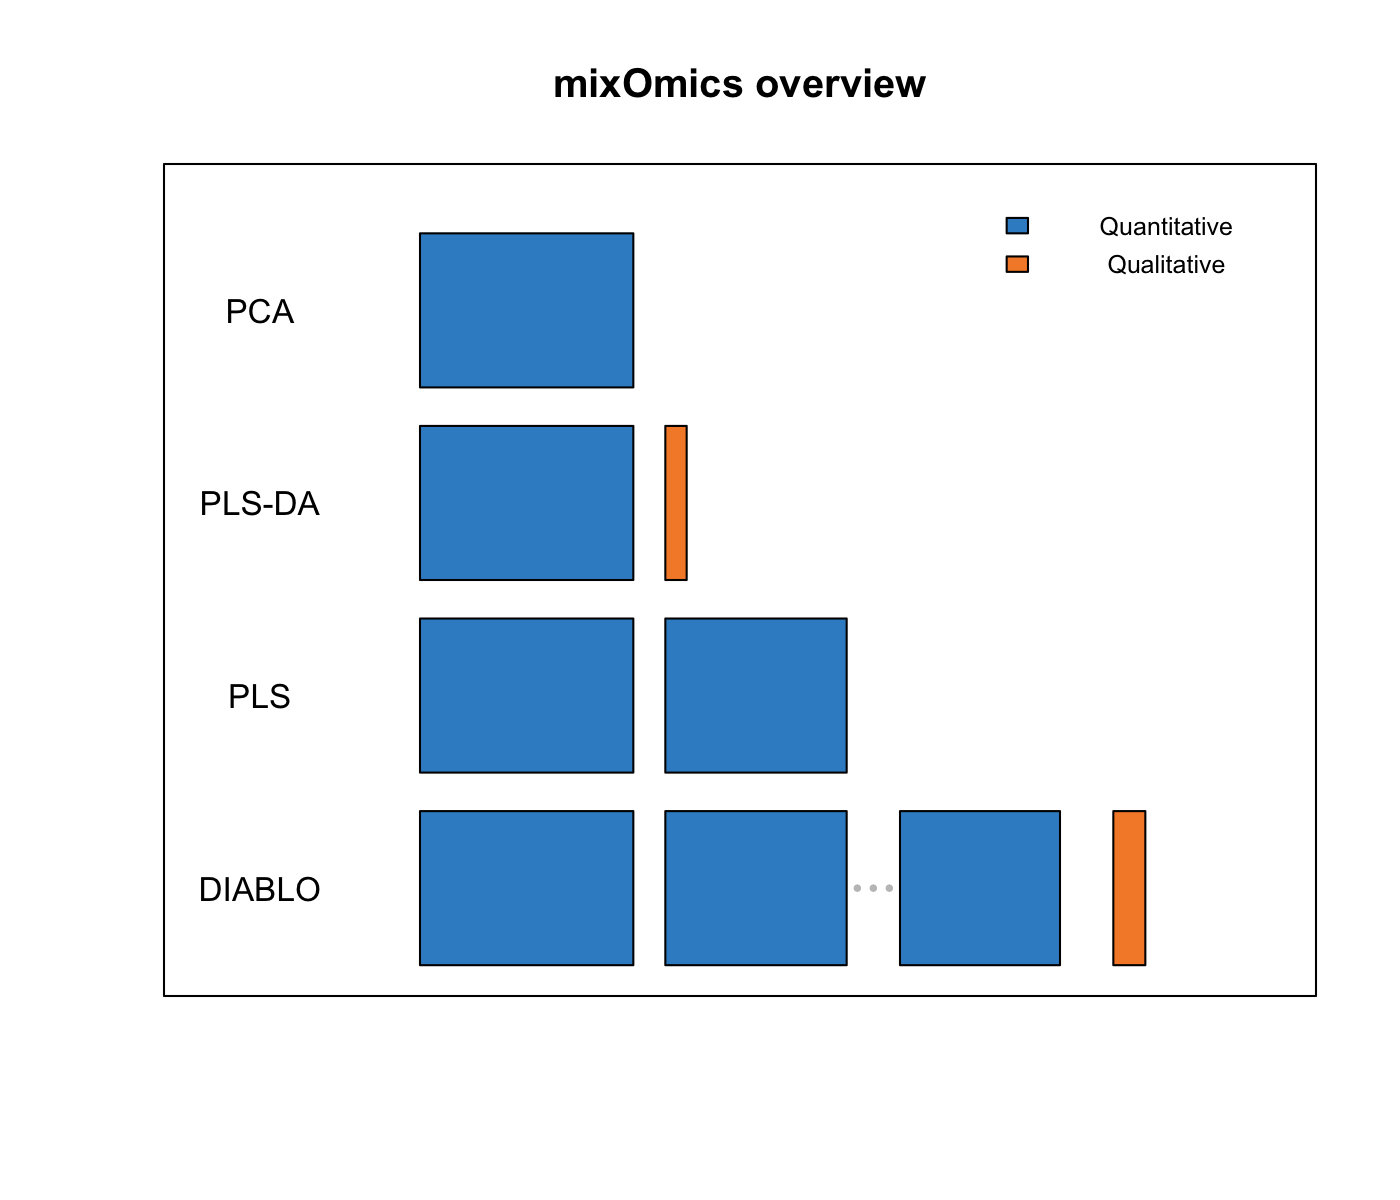
\includegraphics[width=0.5\linewidth]{Figures/overview-1} \end{center}

\begin{figure}

{\centering 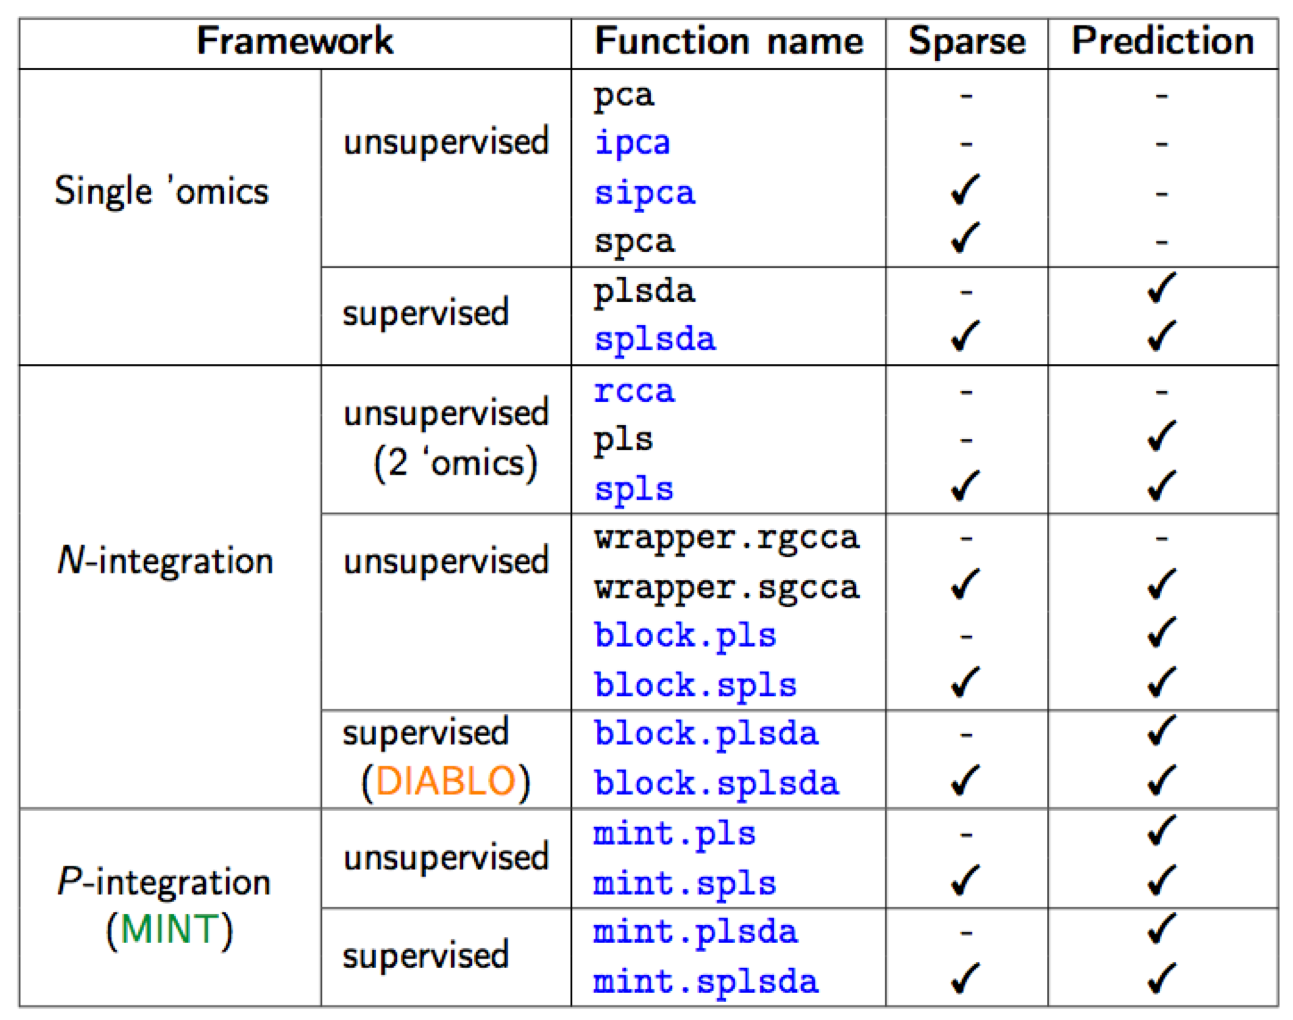
\includegraphics[width=1\linewidth]{XtraFigs/Methods} 

}

\caption{List of methods in mixOmics, sparse indicates methods that perform variable selection}\label{fig:methods}
\end{figure}

\begin{figure}

{\centering 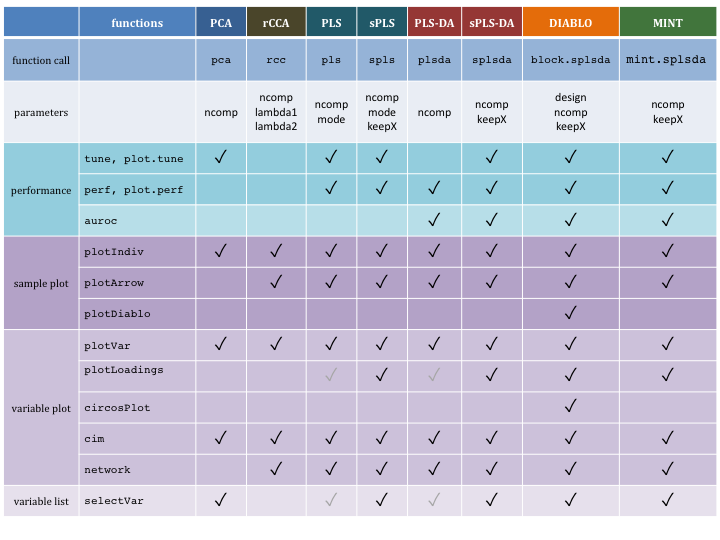
\includegraphics[width=1\linewidth]{XtraFigs/cheatsheet} 

}

\caption{Main functions and parameters of each method}\label{fig:cheatsheet}
\end{figure}

\subsection{Key publications}\label{intro:pubs}

The methods implemented in \texttt{mixOmics} are described in detail in
the following publications. A more extensive list can be found at this
\href{http://mixomics.org/a-propos/publications/}{link}.

\begin{itemize}
\item
  \textbf{Overview and recent integrative methods}: Rohart F., Gautier,
  B, Singh, A, Le Cao, K. A. mixOmics: an
  \href{http://journals.plos.org/ploscompbiol/article?id=10.1371/journal.pcbi.1005752}{R
  package for 'omics feature selection and multiple data integration}.
  \emph{PLoS Comput Biol} 13(11): e1005752.
\item
  \textbf{Graphical outputs for integrative methods}: \citep{Gon12}
  Gonzalez I., Le Cao K.-A., Davis, M.D.~and Dejean S. (2012)
  \href{https://biodatamining.biomedcentral.com/articles/10.1186/1756-0381-5-19}{Insightful
  graphical outputs to explore relationships between two omics data
  sets}. \emph{BioData Mining} 5:19.
\item
  \textbf{DIABLO}: Singh A, Gautier B, Shannon C, Vacher M, Rohart F,
  Tebbutt S, K-A. Le Cao.
  \href{https://www.biorxiv.org/content/early/2018/03/20/067611}{DIABLO
  - multi-omics data integration for biomarker discovery.}
\item
  \textbf{sparse PLS}: Le Cao K.-A., Martin P.G.P, Robert-Granie C. and
  Besse, P. (2009)
  \href{http://www.biomedcentral.com/1471-2105/10/34/}{Sparse Canonical
  Methods for Biological Data Integration: application to a
  cross-platform study}. \emph{BMC Bioinformatics}, 10:34.
\item
  \textbf{sparse PLS-DA}:Le Cao K.-A., Boitard S. and Besse P. (2011)
  \href{https://bmcbioinformatics.biomedcentral.com/articles/10.1186/1471-2105-12-253}{Sparse
  PLS Discriminant Analysis: biologically relevant feature selection and
  graphical displays for multiclass problems}. \emph{BMC
  Bioinformatics}, 22:253.
\item
  \textbf{Multilevel approach for repeated measurements}: Liquet B, Le
  Cao K-A, Hocini H, Thiebaut R (2012).
  \href{https://bmcbioinformatics.biomedcentral.com/articles/10.1186/1471-2105-13-325}{A
  novel approach for biomarker selection and the integration of repeated
  measures experiments from two assays}. \emph{BMC Bioinformatics},
  13:325
\item
  \textbf{sPLS-DA for microbiome data}: Le Cao K-A\(^*\), Costello ME
  \(^*\), Lakis VA , Bartolo F, Chua XY, Brazeilles R and Rondeau P.
  (2016)
  \href{http://journals.plos.org/plosone/article?id=10.1371/journal.pone.0160169}{MixMC:
  Multivariate insights into Microbial Communities}.PLoS ONE 11(8):
  e0160169
\end{itemize}

\section{Outline of this Vignette}\label{outline-of-this-vignette}

\begin{itemize}
\tightlist
\item
  \textbf{Chapter \ref{start}} details some practical aspects to get
  started
\item
  \textbf{Chapter \ref{pca}}: Principal Components Analysis (PCA)
\item
  \textbf{Chapter \ref{plsda}}: Projection to Latent Structure -
  Discriminant Analysis (PLS-DA)
\item
  \textbf{Chapter \ref{pls}}: Projection to Latent Structures (PLS)
\item
  \textbf{Chapter \ref{diablo}}: Integrative analysis for multiple data
  sets (DIABLO)
\end{itemize}

Each of the methods chapter has the following outline:

\begin{enumerate}
\def\labelenumi{\arabic{enumi}.}
\tightlist
\item
  Type of biological question to be answered
\item
  Brief description of an illustrative data set
\item
  Principle of the method
\item
  Quick start of the method with the main functions and arguments
\item
  To go further: customized plots, additional graphical outputs and
  tuning parameters
\item
  FAQ
\end{enumerate}

\section{Other methods not covered in this
vignette}\label{other-methods-not-covered-in-this-vignette}

Other methods not covered in this document are described on our website
and the following references:

\begin{itemize}
\item
  \href{http://www.mixOmics.org}{regularised Canonical Correlation
  Analysis}, see the \textbf{Methods} and \textbf{Case study} tabs, and
  \citep{Gon08} that describes CCA for large data sets.
\item
  \href{http://www.mixOmics.org/mixmc}{Microbiome (16S, shotgun
  metagenomics) data analysis}, see also \citep{Lec16} and
  \href{http://mixomics.org/mixkernel}{kernel integration for microbiome
  data}. The latter is in collaboration with Drs J Mariette and Nathalie
  Villa-Vialaneix (INRA Toulouse, France), an example is provided for
  the Tara ocean metagenomics and environmental data, see also
  \citep{Mar17}.
\item
  \href{http://mixomics.org/mixmint/}{MINT} or P-integration to
  integrate independently generated transcriptomics data sets. An
  example in stem cells studies, see also \citep{Roh16}.
\end{itemize}

\chapter{Let's get started}\label{start}

\section{Installation}\label{installation}

First, install the latest \texttt{mixOmics} version:

\begin{Shaded}
\begin{Highlighting}[]
\CommentTok{# in bioconductor:}
\CommentTok{# try http:// if https:// URLs are not supported}
\KeywordTok{source}\NormalTok{(}\StringTok{"https://bioconductor.org/biocLite.R"}\NormalTok{)}
\KeywordTok{biocLite}\NormalTok{(}\StringTok{'mixOmics'}\NormalTok{)}
\end{Highlighting}
\end{Shaded}

The \texttt{mixOmics} package should directly import the following
packages:
\texttt{igraph,\ rgl,\ ellipse,\ corpcor,\ RColorBrewer,\ plyr,\ parallel,\ dplyr,\ tidyr,\ reshape2,\ methods,\ matrixStats,\ rARPACK,\ gridExtra}.
For \emph{apple mac users}, if you are unable to install the imported
library \texttt{rgl}, you will need to install the
\href{https://www.xquartz.org}{XQuartz software} first.

\section{Load the package}\label{start:upload}

\begin{Shaded}
\begin{Highlighting}[]
\KeywordTok{library}\NormalTok{(mixOmics)}
\end{Highlighting}
\end{Shaded}

Check that there is no error when loading the package, especially for
the \texttt{rgl} library (see above).

\section{Upload data}\label{upload-data}

The examples we give in this vignette use data that are already part of
the package. To upload your own data, check first that your working
directory is set, then read your data from a \texttt{.txt} or
\texttt{.csv} format, either by using \textbf{File \textgreater{} Import
Dataset} in RStudio or via one of these command lines:

\begin{Shaded}
\begin{Highlighting}[]
\CommentTok{# from csv file}
\NormalTok{data <-}\StringTok{ }\KeywordTok{read.csv}\NormalTok{(}\StringTok{"your_data.csv"}\NormalTok{, }\DataTypeTok{row.names =} \DecValTok{1}\NormalTok{, }\DataTypeTok{header =} \OtherTok{TRUE}\NormalTok{)}

\CommentTok{# from txt file}
\NormalTok{data <-}\StringTok{ }\KeywordTok{read.table}\NormalTok{(}\StringTok{"your_data.txt"}\NormalTok{, }\DataTypeTok{header =} \OtherTok{TRUE}\NormalTok{)}
\end{Highlighting}
\end{Shaded}

For more details about the arguments used to modify those functions,
type \texttt{?read.csv} or \texttt{?read.table} in the R console.

\section{\texorpdfstring{Quick start in
\texttt{mixOmics}}{Quick start in mixOmics}}\label{start:PCA}

Each analysis should follow this workflow:

\begin{enumerate}
\def\labelenumi{\arabic{enumi}.}
\tightlist
\item
  Run the method
\item
  Graphical representation of the samples
\item
  Graphical representation of the variables
\end{enumerate}

Then use your critical thinking and additional functions and visual
tools to make sense of your data! (some of which are listed in
\ref{intro:overview}) and will be described in the next Chapters.

For instance, for Principal Components Analysis, we first load the data:

\begin{Shaded}
\begin{Highlighting}[]
\KeywordTok{data}\NormalTok{(nutrimouse)}
\NormalTok{X <-}\StringTok{ }\NormalTok{nutrimouse}\OperatorTok{$}\NormalTok{gene}
\end{Highlighting}
\end{Shaded}

Then use the following steps:

\begin{Shaded}
\begin{Highlighting}[]
\NormalTok{MyResult.pca <-}\StringTok{ }\KeywordTok{pca}\NormalTok{(X)  }\CommentTok{# 1 Run the method}
\KeywordTok{plotIndiv}\NormalTok{(MyResult.pca) }\CommentTok{# 2 Plot the samples}
\end{Highlighting}
\end{Shaded}

\begin{center}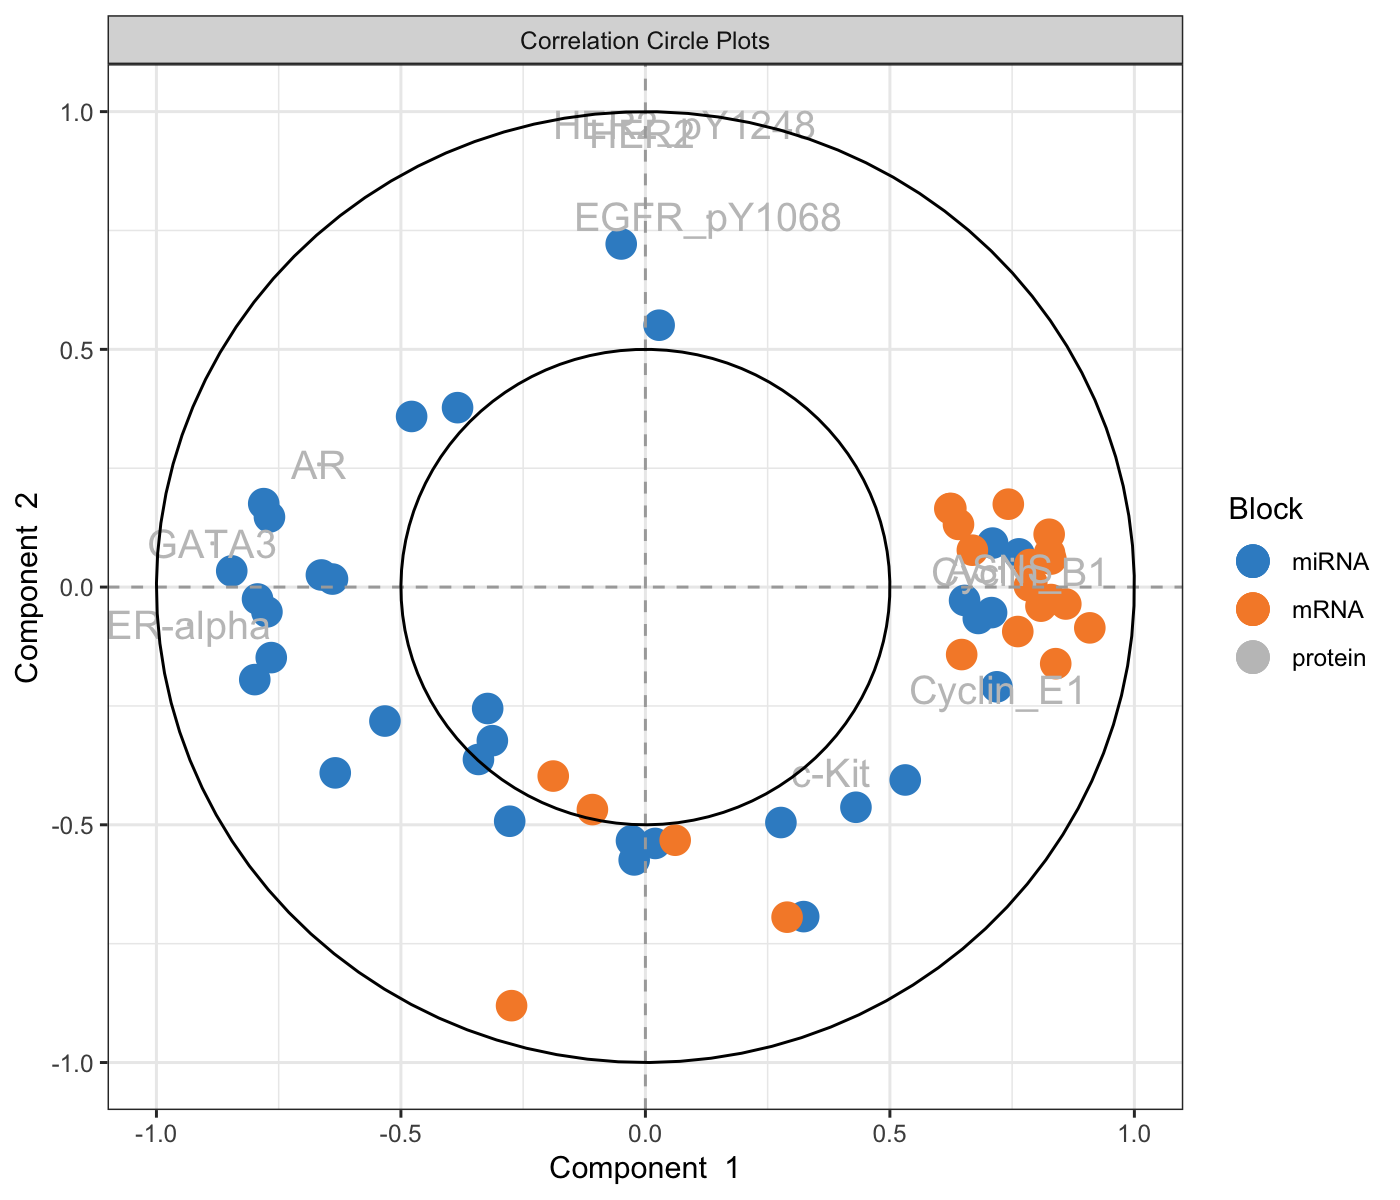
\includegraphics[width=0.5\linewidth]{Figures/unnamed-chunk-5-1} \end{center}

\begin{Shaded}
\begin{Highlighting}[]
\KeywordTok{plotVar}\NormalTok{(MyResult.pca)   }\CommentTok{# 3 Plot the variables}
\end{Highlighting}
\end{Shaded}

\begin{center}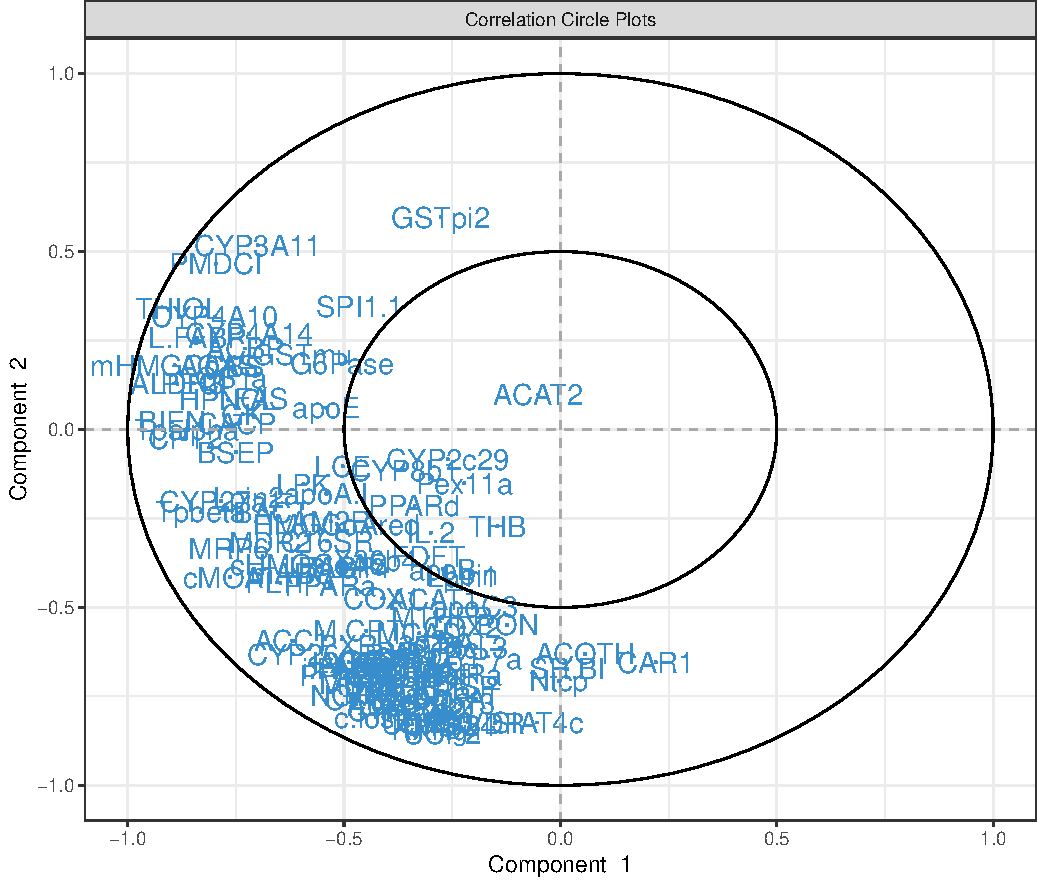
\includegraphics[width=0.5\linewidth]{Figures/unnamed-chunk-5-2} \end{center}

This is only a first quick-start, there will be many avenues you can
take to deepen your exploratory and integrative analyses. The package
proposes several methods to perform variable, or feature selection to
identify the relevant information from rather large omics data sets. The
sparse methods are listed in the Table in \ref{intro:overview}.

Following our example here, sparse PCA can be applied to select the top
5 variables contributing to each of the two components in PCA. The user
specifies the number of variables to selected on each component, for
example here 5 variables are selected on each of the first two
components (\texttt{keepX=c(5,5)}):

\begin{Shaded}
\begin{Highlighting}[]
\NormalTok{MyResult.spca <-}\StringTok{ }\KeywordTok{spca}\NormalTok{(X, }\DataTypeTok{keepX=}\KeywordTok{c}\NormalTok{(}\DecValTok{5}\NormalTok{,}\DecValTok{5}\NormalTok{)) }\CommentTok{# 1 Run the method}
\KeywordTok{plotIndiv}\NormalTok{(MyResult.spca)               }\CommentTok{# 2 Plot the samples}
\end{Highlighting}
\end{Shaded}

\begin{center}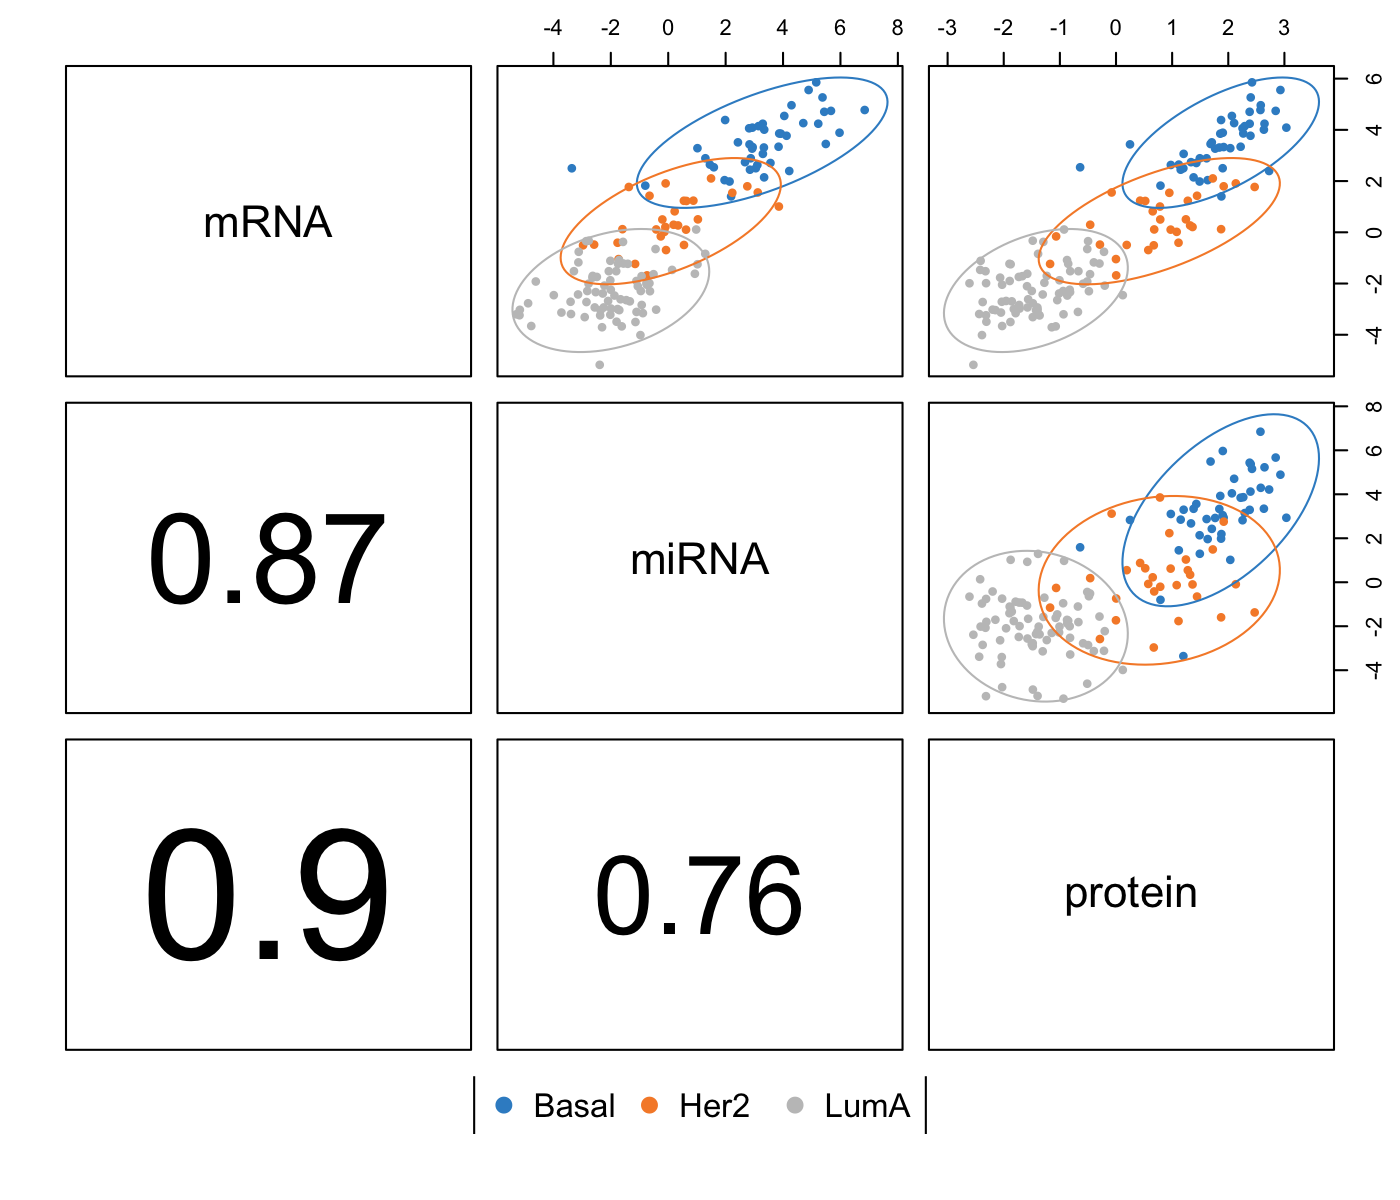
\includegraphics[width=0.5\linewidth]{Figures/unnamed-chunk-6-1} \end{center}

\begin{Shaded}
\begin{Highlighting}[]
\KeywordTok{plotVar}\NormalTok{(MyResult.spca)                 }\CommentTok{# 3 Plot the variables}
\end{Highlighting}
\end{Shaded}

\begin{center}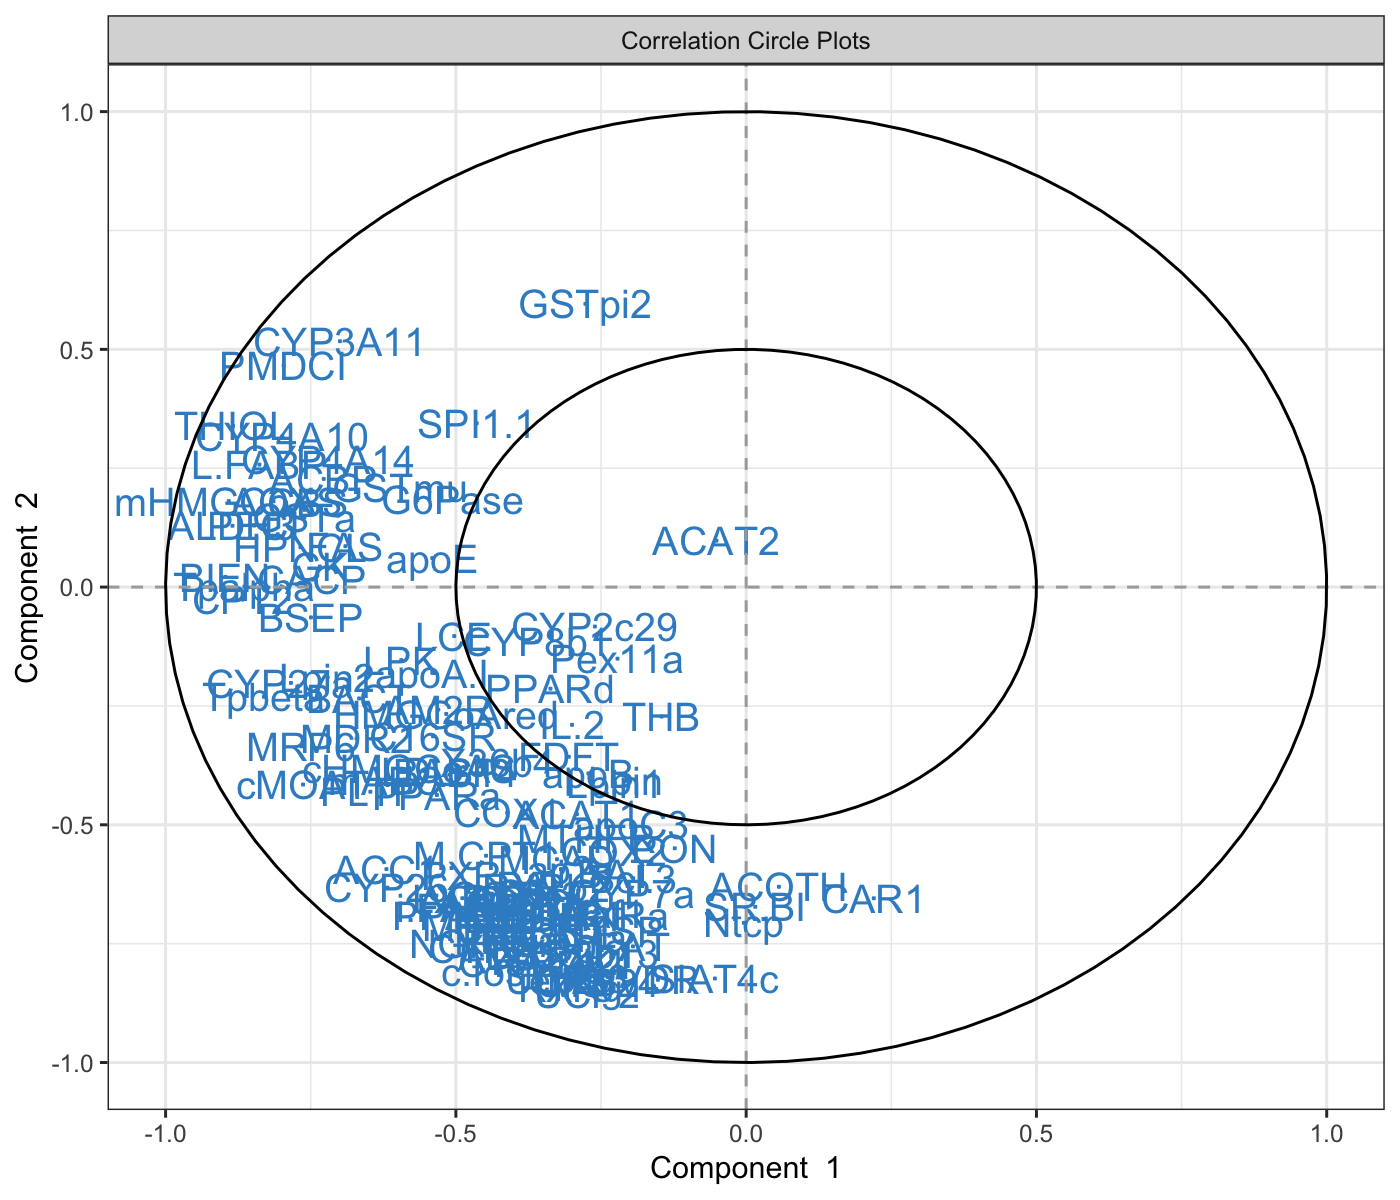
\includegraphics[width=0.5\linewidth]{Figures/unnamed-chunk-6-2} \end{center}

You can see know that we have considerably reduced the number of genes
in the \texttt{plotVar} correlation circle plot.

Do not stop here! We are not done yet. You can enhance your analyses
with the following:

\begin{itemize}
\item
  Have a look at our manual and each of the functions and their
  examples, e.g. \texttt{?pca}, \texttt{?plotIndiv}, \texttt{?sPCA},
  \ldots{}
\item
  Run the examples from the help file using the \texttt{example}
  function: \texttt{example(pca)}, \texttt{example(plotIndiv)}, \ldots{}
\item
  Have a look at out \href{http://www.mixomics.org}{website} that
  features many tutorials and case studies,
\item
  Keep reading this vignette, this is \emph{just the beginning!}
\end{itemize}

\chapter{Principal Component Analysis (PCA)}\label{pca}

\begin{center}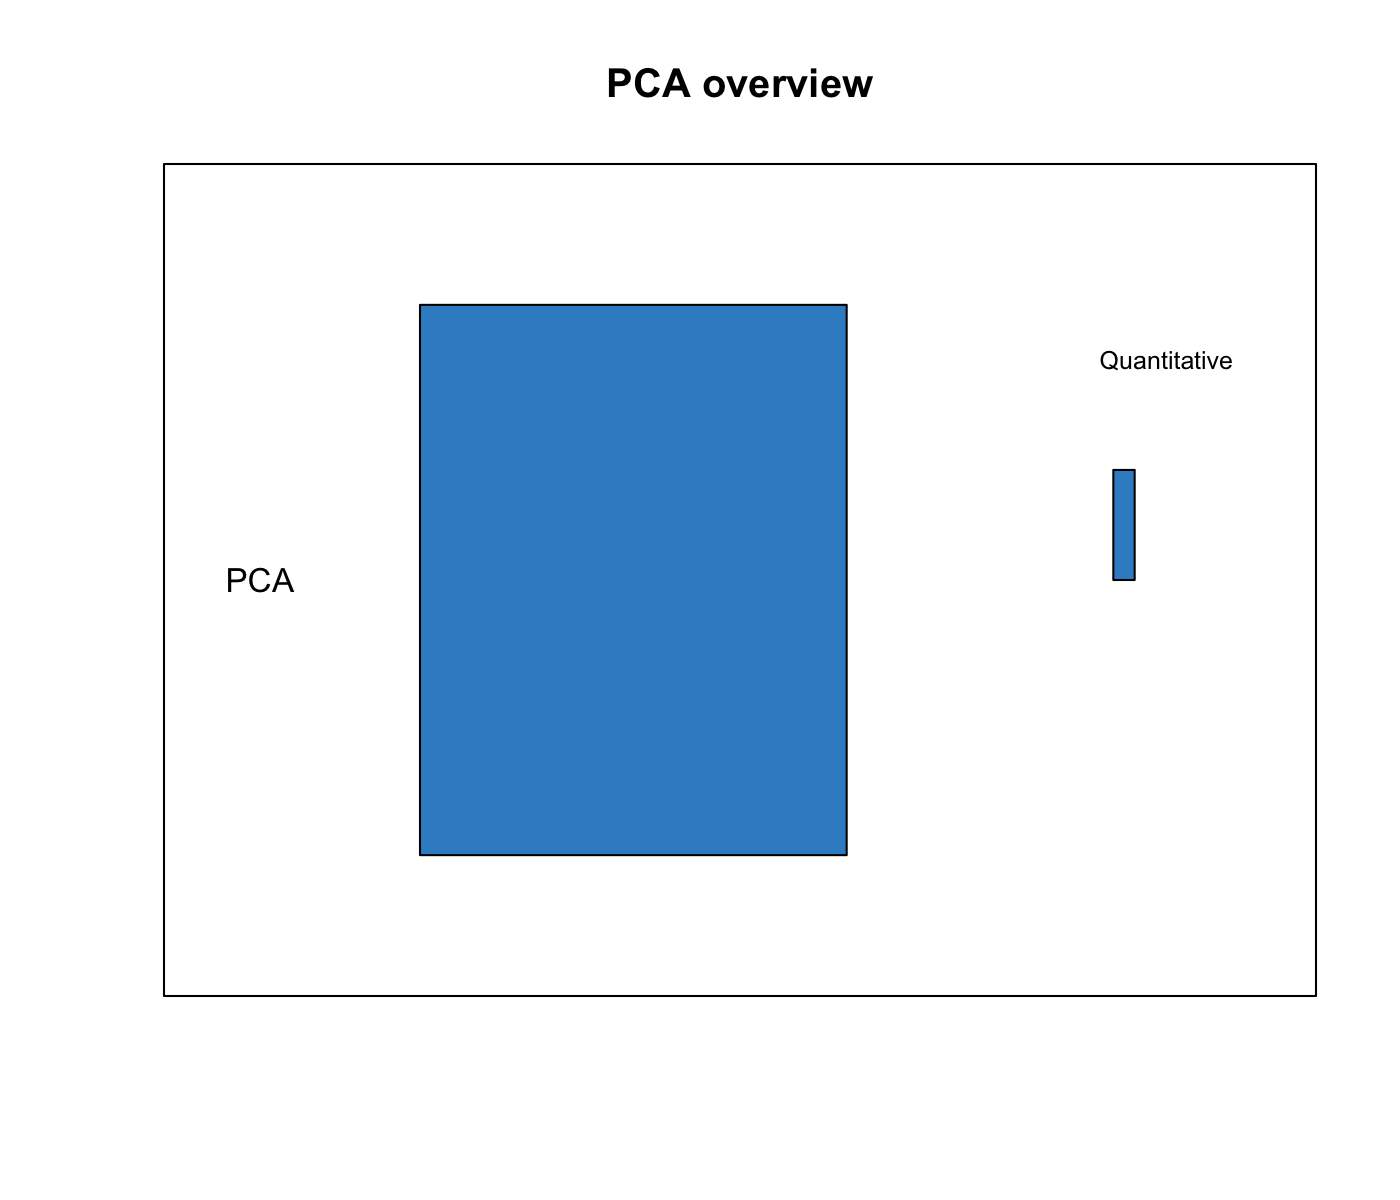
\includegraphics[width=0.5\linewidth]{Figures/overview-PCA-1} \end{center}

\section{Biological question}\label{biological-question}

{ \emph{I would like to identify the major sources of variation in my
data and itdentify whether such sources of variation correspond to
biological conditions, or experimental bias. I would like visualise
trends or patterns between samples,whether they `naturally' cluster
according to known biological conditions.} }

\section{\texorpdfstring{The \texttt{liver.toxicity}
study}{The liver.toxicity study}}\label{the-liver.toxicity-study}

The \texttt{liver.toxicity} is a list in the package that contains:

\begin{itemize}
\item
  \texttt{gene}: a data frame with 64 rows and 3116 columns,
  corresponding to the expression levels of 3,116 genes measured on 64
  rats.
\item
  \texttt{clinic}: a data frame with 64 rows and 10 columns,
  corresponding to the measurements of 10 clinical variables on the same
  64 rats.
\item
  \texttt{treatment}: data frame with 64 rows and 4 columns, indicating
  the treatment information of the 64 rats, such as doses of
  acetaminophen and times of necropsy.
\item
  \texttt{gene.ID}: a data frame with 3116 rows and 2 columns,
  indicating geneBank IDs of the annotated genes.
\end{itemize}

More details are available at \texttt{?liver.toxicity}.

To illustrate PCA, we focus on the expression levels of the genes in the
data frame \texttt{liver.toxicity\$gene}. Some of the terms mentioned
below are listed in \ref{intro:background}.

\section{Principle of PCA}\label{principle-of-pca}

The aim of PCA \citep{Jol05} is to reduce the dimensionality of the data
whilst retaining as much information as possible. `Information' is
referred here as \emph{variance}. The idea is to create uncorrelated
artificial variables called \emph{principal components} (PCs) that
combine in a linear manner the original (possibly correlated) variables
(e.g.~genes, metabolites, etc.).

Dimension reduction is achieved by projecting the data into the space
spanned by the principal components (PC). In practice, it means that
each sample is assigned a score on each new PC dimension - this score is
calculated as a linear combination of the original variables to which a
weight is applied. The weights of each of the original variables are
stored in the so-called \emph{loading vectors} associated to each PC.
The dimension of the data is reduced by projecting the data into the
smaller subspace spanned by the PCs, while capturing the largest sources
of variation between samples.

The principal components are obtained by maximising the
variance-covariance matrix of the data. To that end, we calculate the
eigenvectors/eigenvalues of the variance-covariance matrix, often via
singular value decomposition when the number of variables is very large.
The data are usually centred (\texttt{center\ =\ TRUE}), and sometimes
scaled (\texttt{scale\ =\ TRUE}) in the method. The latter is especially
advised in the case where the variance is not homogeneous across
variables.

The first PC is defined as the linear combination of the original
variables that explains the greatest amount of variation. The second PC
is then defined as the linear combination of the original variables that
accounts for the greatest amount of the remaining variation subject of
being orthogonal (uncorrelated) to the first component. Subsequent
components are defined likewise for the other PCA dimensions. The user
must therefore report how much information is explained by the first PCs
as these are used to graphically represent the PCA outputs.

\section{Load the data}\label{load-the-data}

We first load the data from the package. See \ref{start:upload} to
upload your own data.

\begin{Shaded}
\begin{Highlighting}[]
\KeywordTok{library}\NormalTok{(mixOmics)}
\KeywordTok{data}\NormalTok{(liver.toxicity)}
\NormalTok{X <-}\StringTok{ }\NormalTok{liver.toxicity}\OperatorTok{$}\NormalTok{gene}
\end{Highlighting}
\end{Shaded}

\section{Quick start}\label{quick-start}

\begin{Shaded}
\begin{Highlighting}[]
\NormalTok{MyResult.pca <-}\StringTok{ }\KeywordTok{pca}\NormalTok{(X)     }\CommentTok{# 1 Run the method}
\KeywordTok{plotIndiv}\NormalTok{(MyResult.pca)    }\CommentTok{# 2 Plot the samples}
\end{Highlighting}
\end{Shaded}

\begin{Shaded}
\begin{Highlighting}[]
\KeywordTok{plotVar}\NormalTok{(MyResult.pca)      }\CommentTok{# 3 Plot the variables}
\end{Highlighting}
\end{Shaded}

If you were to run \texttt{pca} with this minimal code, you would be
using the following default values:

\begin{itemize}
\tightlist
\item
  \texttt{ncomp\ =2}: the first two principal components are calculated
  and are used for graphical outputs;
\item
  \texttt{center\ =\ TRUE}: data are centred (mean = 0)
\item
  \texttt{scale\ =\ FALSE}: data are not scaled. If
  \texttt{scale\ =\ TRUE} standardizes each variable (variance = 1).
\end{itemize}

Other arguments can also be chosen, see \texttt{?pca}.

This example was shown in Chapter \ref{start:PCA}. The two plots are not
extremely meaningful as specific sample patterns should be further
investigated and the variable correlation circle plot plot contains too
many variables to be easily interpreted. Let's improve those graphics as
shown below to improve interpretation.

\section{To go further}\label{to-go-further}

\subsection{Customize plots}\label{customize-plots}

Plots can be customized using numerous options in \texttt{plotIndiv} and
\texttt{plotVar}. For instance, even if PCA does not take into account
any information regarding the known group membership of each sample, we
can include such information on the sample plot to visualize any
`natural' cluster that may corresponds to biological conditions.

Here is an example where we include the sample groups information with
the argument \texttt{group}:

\begin{Shaded}
\begin{Highlighting}[]
\KeywordTok{plotIndiv}\NormalTok{(MyResult.pca, }\DataTypeTok{group =}\NormalTok{ liver.toxicity}\OperatorTok{$}\NormalTok{treatment}\OperatorTok{$}\NormalTok{Dose.Group, }
          \DataTypeTok{legend =} \OtherTok{TRUE}\NormalTok{)}
\end{Highlighting}
\end{Shaded}

\begin{center}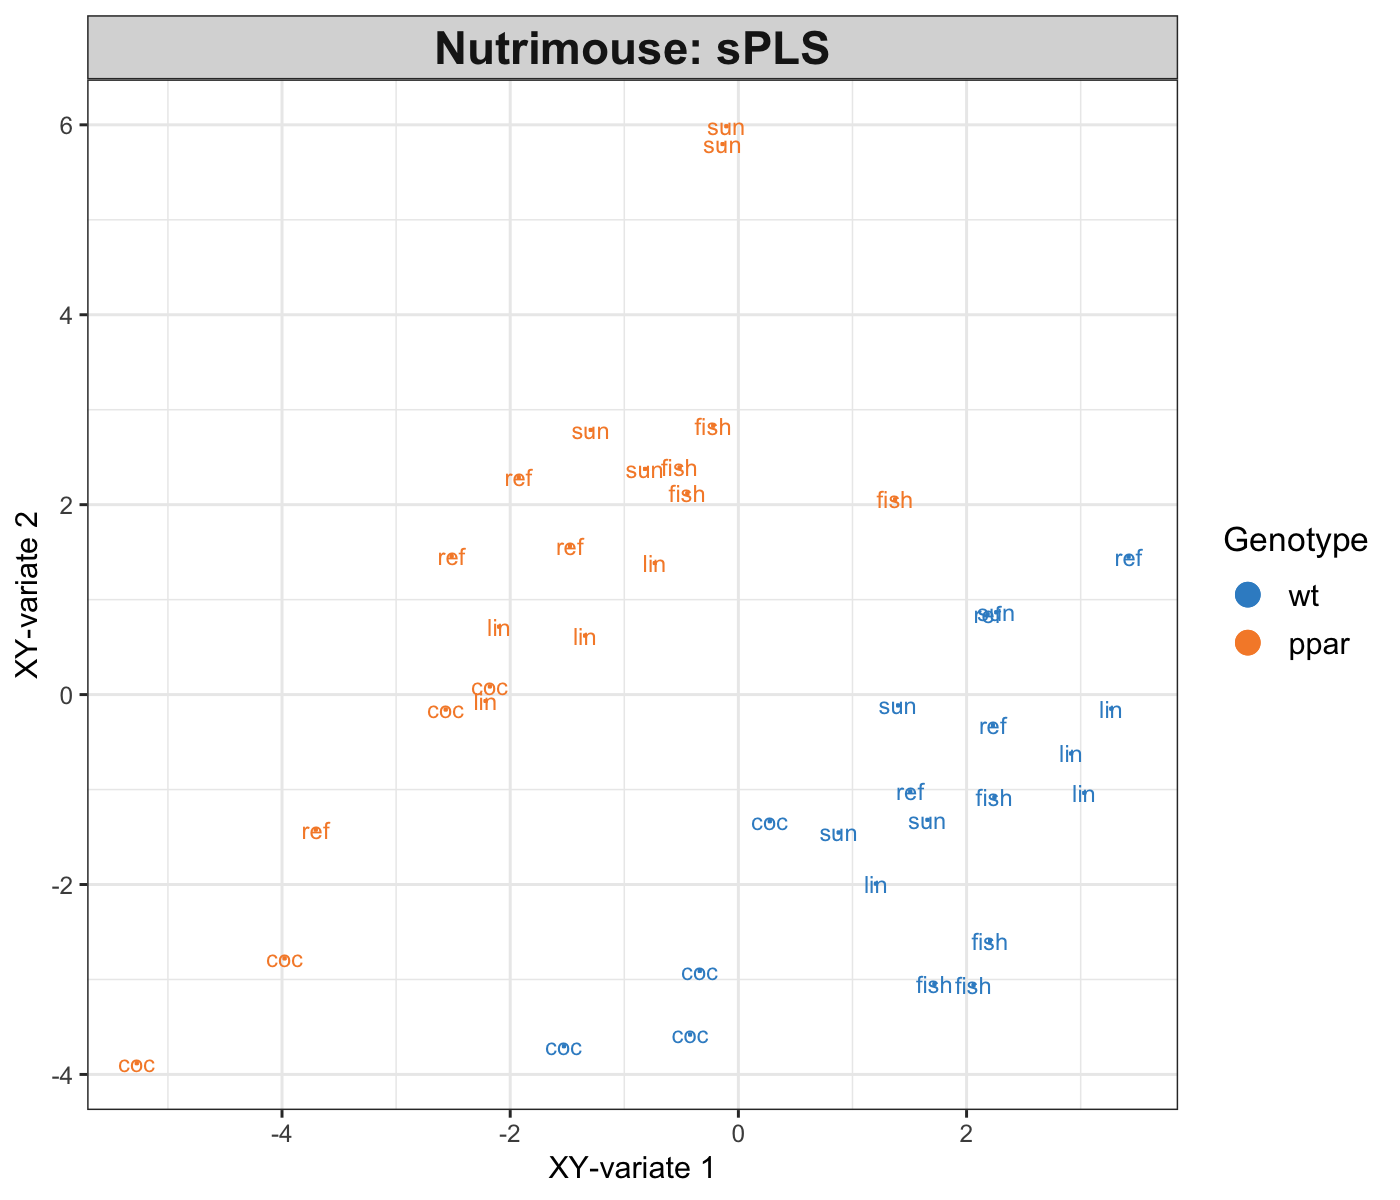
\includegraphics[width=0.5\linewidth]{Figures/unnamed-chunk-3-1} \end{center}

Additionally, two factors can be displayed using both colours (argument
\texttt{group}) and symbols (argument \texttt{pch}). For example here we
display both Dose and Time of exposure and improve the title and legend:

\begin{Shaded}
\begin{Highlighting}[]
\KeywordTok{plotIndiv}\NormalTok{(MyResult.pca, }\DataTypeTok{ind.names =} \OtherTok{FALSE}\NormalTok{,}
          \DataTypeTok{group =}\NormalTok{ liver.toxicity}\OperatorTok{$}\NormalTok{treatment}\OperatorTok{$}\NormalTok{Dose.Group,}
          \DataTypeTok{pch =} \KeywordTok{as.factor}\NormalTok{(liver.toxicity}\OperatorTok{$}\NormalTok{treatment}\OperatorTok{$}\NormalTok{Time.Group),}
          \DataTypeTok{legend =} \OtherTok{TRUE}\NormalTok{, }\DataTypeTok{title =} \StringTok{'Liver toxicity: genes, PCA comp 1 - 2'}\NormalTok{,}
          \DataTypeTok{legend.title =} \StringTok{'Dose'}\NormalTok{, }\DataTypeTok{legend.title.pch =} \StringTok{'Exposure'}\NormalTok{)}
\end{Highlighting}
\end{Shaded}

\begin{center}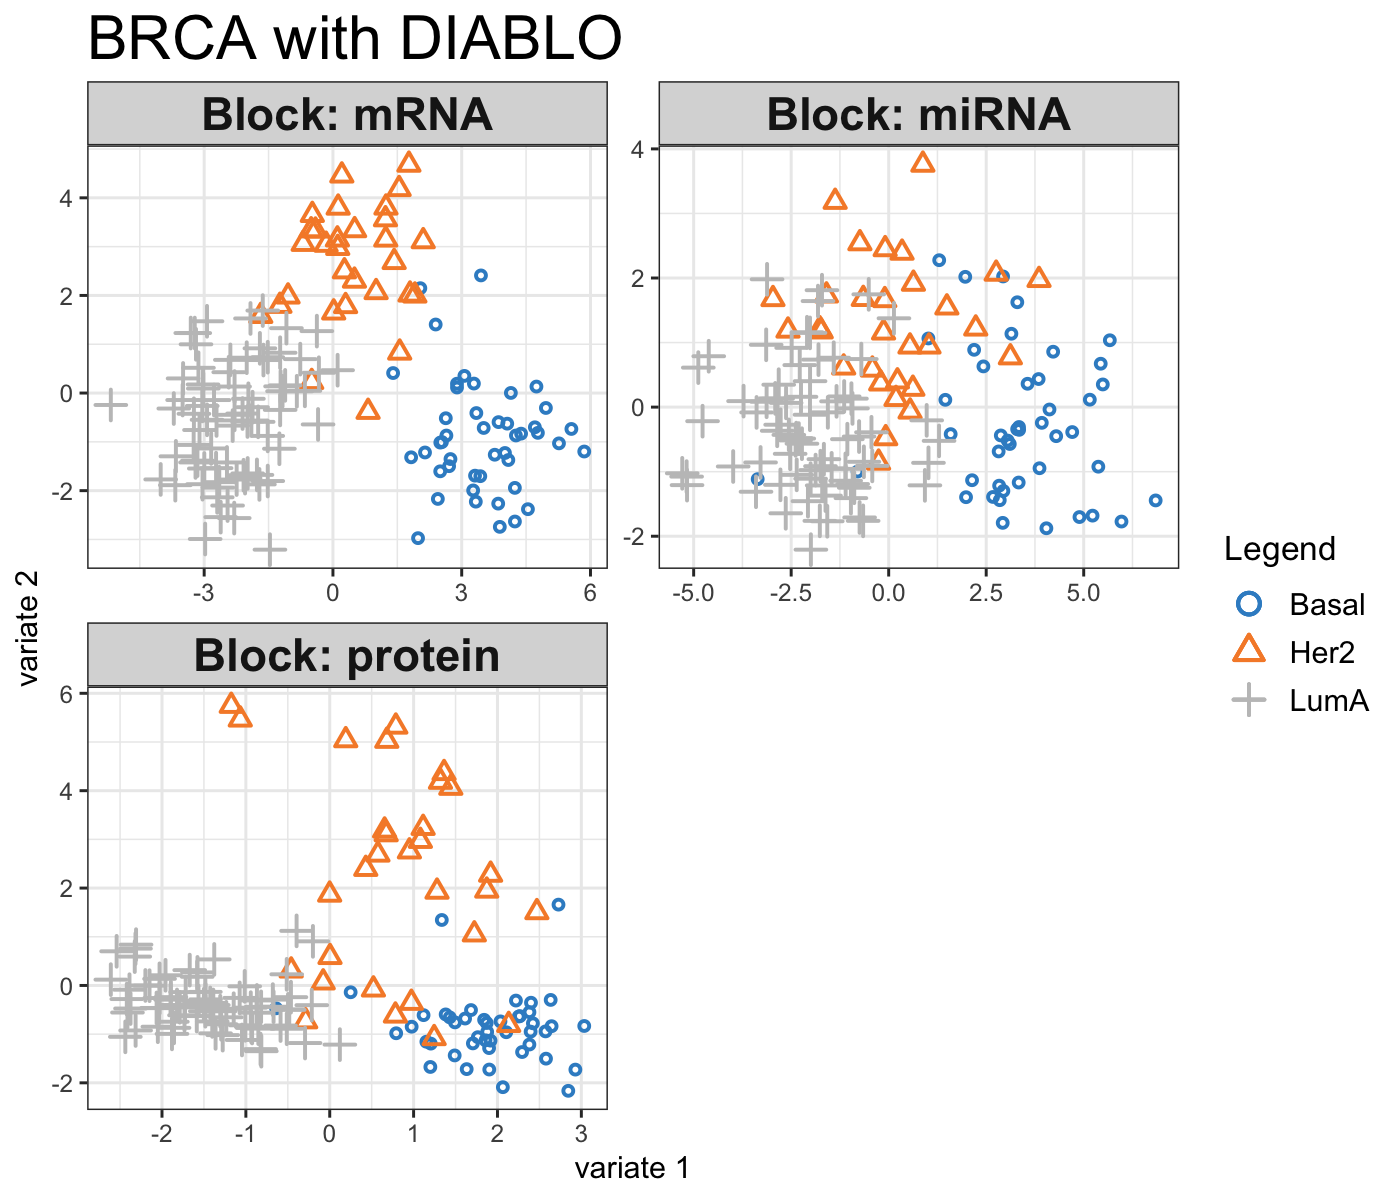
\includegraphics[width=0.5\linewidth]{Figures/unnamed-chunk-4-1} \end{center}

By including information related to the dose of acetaminophen and time
of exposure enables us to see a cluster of low dose samples (blue and
orange, top left at 50 and 100mg respectively), whereas samples with
high doses (1500 and 2000mg in grey and green respectively) are more
scattered, but highlight an exposure effect.

To display the results on other components, we can change the
\texttt{comp} argument provided we have requested enough components to
be calculated. Here is our second PCA with 3 components:

\begin{Shaded}
\begin{Highlighting}[]
\NormalTok{MyResult.pca2 <-}\StringTok{ }\KeywordTok{pca}\NormalTok{(X, }\DataTypeTok{ncomp =} \DecValTok{3}\NormalTok{)}
\KeywordTok{plotIndiv}\NormalTok{(MyResult.pca2, }\DataTypeTok{comp =} \KeywordTok{c}\NormalTok{(}\DecValTok{1}\NormalTok{,}\DecValTok{3}\NormalTok{), }\DataTypeTok{legend =} \OtherTok{TRUE}\NormalTok{,}
          \DataTypeTok{group =}\NormalTok{ liver.toxicity}\OperatorTok{$}\NormalTok{treatment}\OperatorTok{$}\NormalTok{Time.Group,}
          \DataTypeTok{title =} \StringTok{'Multidrug transporter, PCA comp 1 - 3'}\NormalTok{)}
\end{Highlighting}
\end{Shaded}

\begin{center}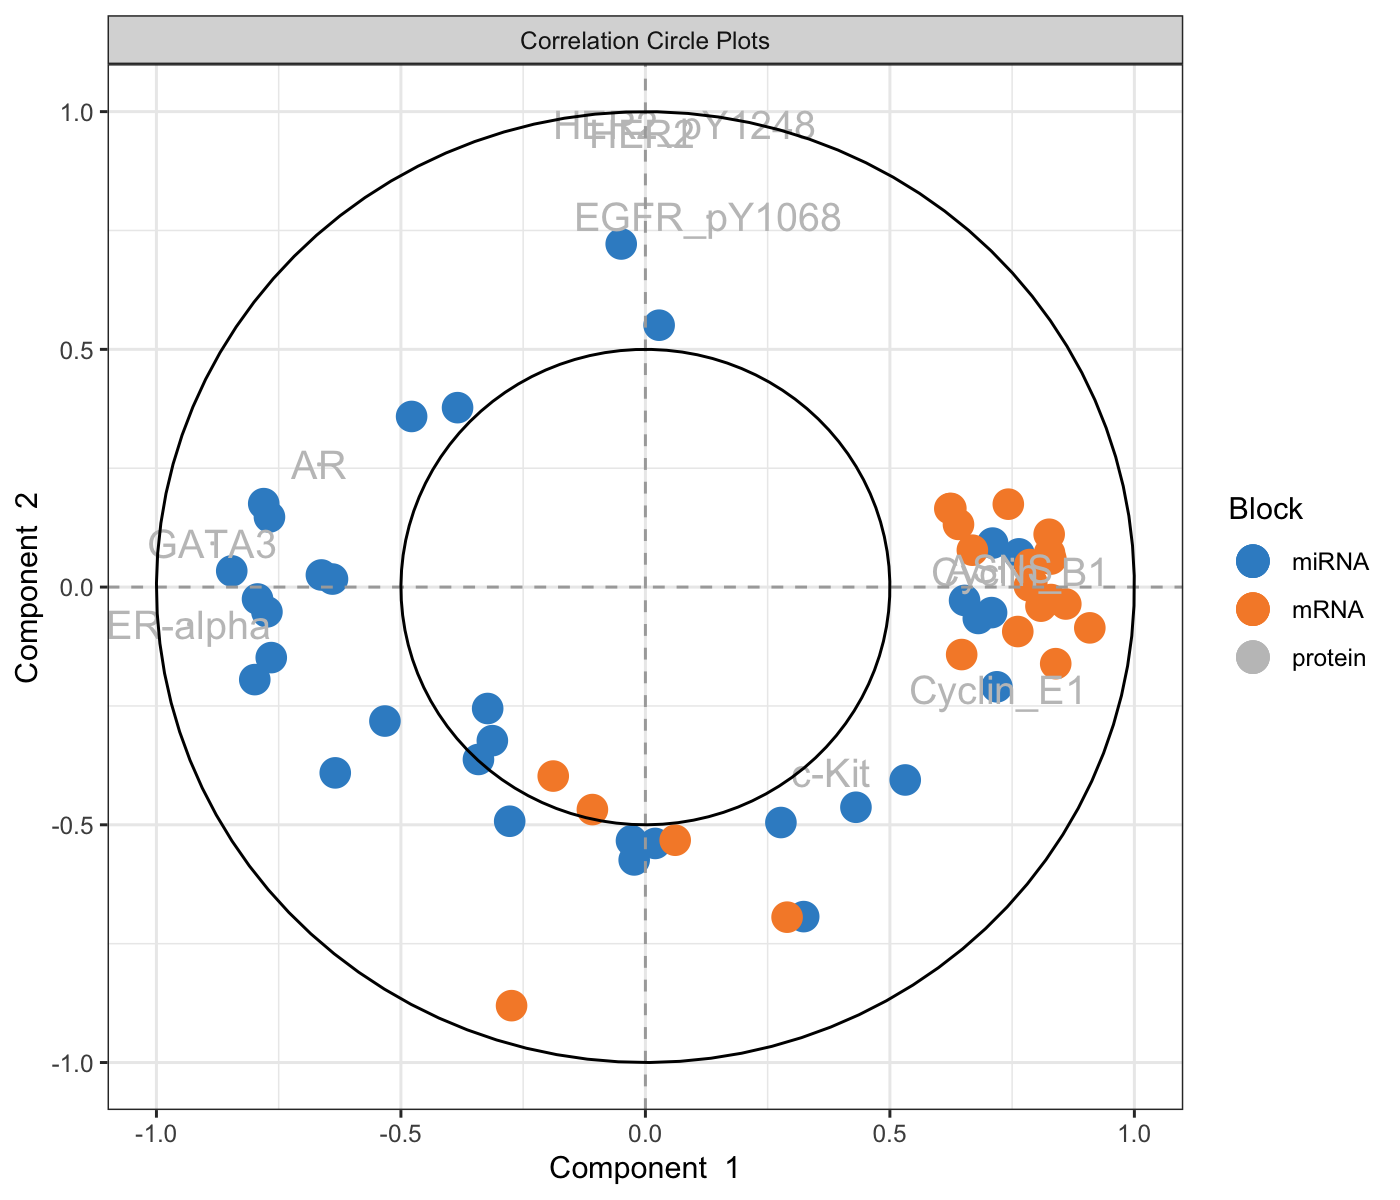
\includegraphics[width=0.5\linewidth]{Figures/unnamed-chunk-5-1} \end{center}

Here, the 3rd component on the y-axis clearly highlights a time of
exposure effect.

\subsection{Amount of variance explained and choice of number of
components}\label{amount-of-variance-explained-and-choice-of-number-of-components}

The amount of variance explained can be extracted with the following: a
screeplot or the actual numerical proportions of explained variance, and
cumulative proportion.

\begin{Shaded}
\begin{Highlighting}[]
\KeywordTok{plot}\NormalTok{(MyResult.pca2)}
\end{Highlighting}
\end{Shaded}

\begin{center}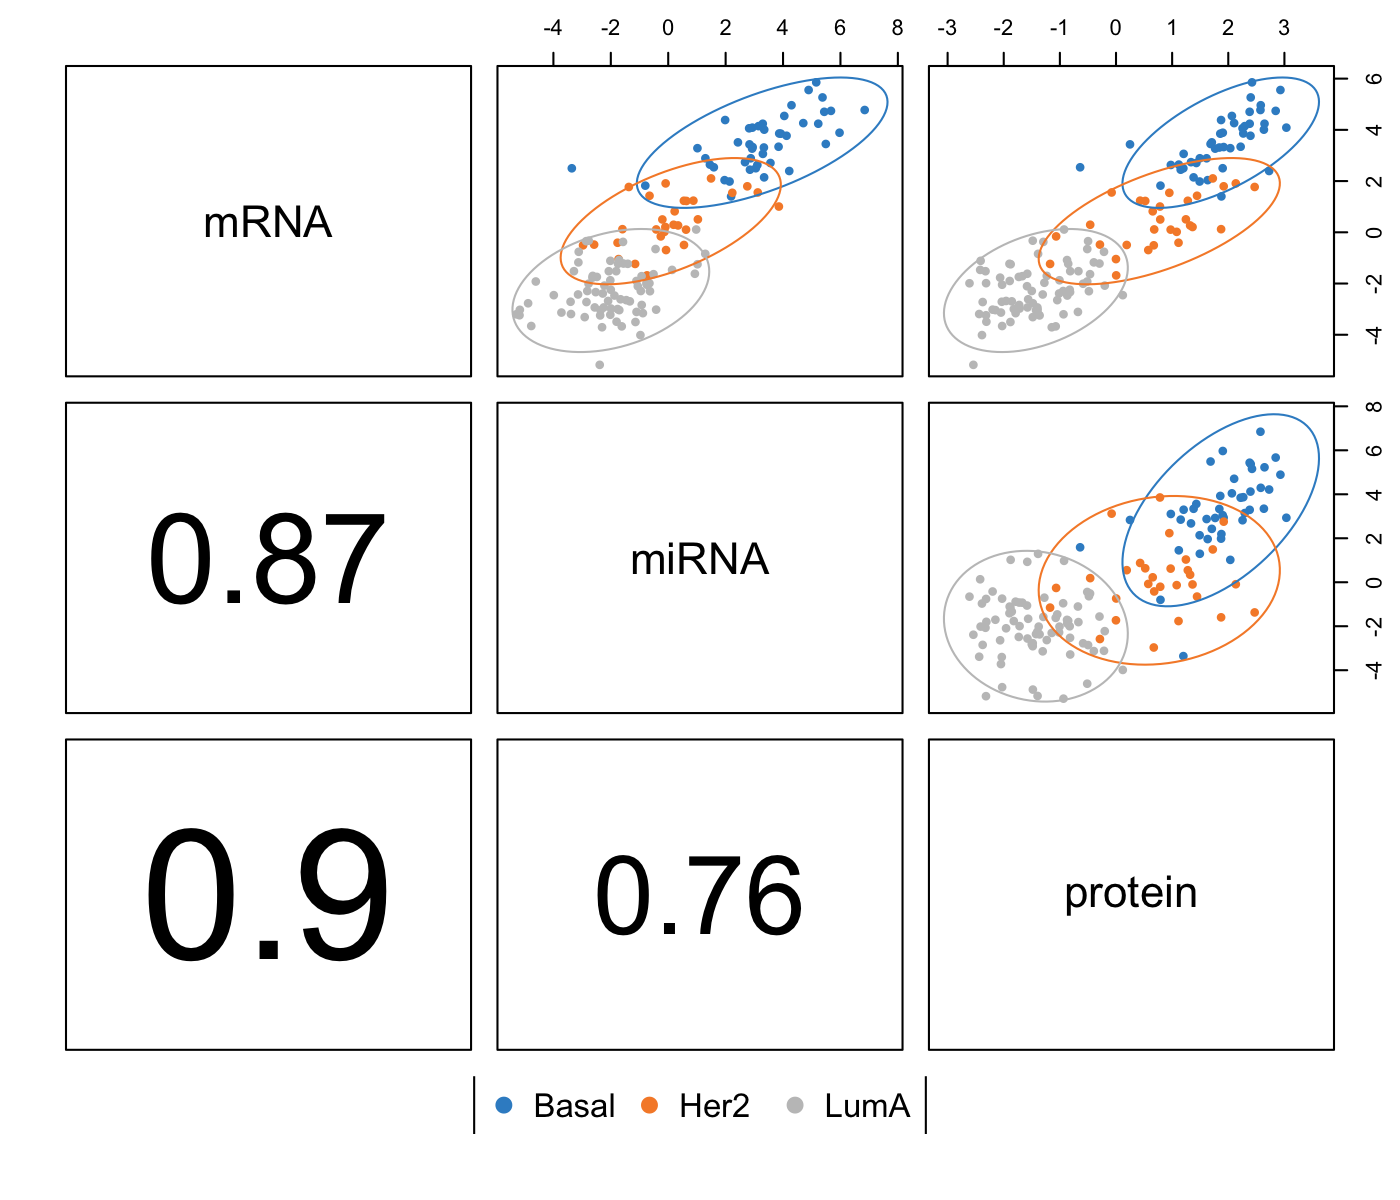
\includegraphics[width=0.5\linewidth]{Figures/unnamed-chunk-6-1} \end{center}

\begin{Shaded}
\begin{Highlighting}[]
\NormalTok{MyResult.pca2}
\end{Highlighting}
\end{Shaded}

\begin{verbatim}
## Eigenvalues for the first 3 principal components, see object$sdev^2: 
##       PC1       PC2       PC3 
## 17.971416  9.079234  4.567709 
## 
## Proportion of explained variance for the first 3 principal components, see object$explained_variance: 
##        PC1        PC2        PC3 
## 0.35684128 0.18027769 0.09069665 
## 
## Cumulative proportion explained variance for the first 3 principal components, see object$cum.var: 
##       PC1       PC2       PC3 
## 0.3568413 0.5371190 0.6278156 
## 
##  Other available components: 
##  -------------------- 
##  loading vectors: see object$rotation
\end{verbatim}

There is no clear guidelines on how many components should be included
in PCA: it is data dependent and the level of noise. We often look at
the `elbow' on the screeplot above as an indicator that the addition of
PCs does not drastically contribute to explain the remainder variance.

\subsection{Other useful plots}\label{other-useful-plots}

We can also have a look at the variable coefficients in each component
with the loading vectors. The loading weights are represented in
decreasing order from bottom to top in \texttt{plotLoadings}. Their
absolute value indicates the importance of each variable to define each
PC, as represented by the length of each bar. See \texttt{?plotLoadings}
to change the arguments.

\begin{Shaded}
\begin{Highlighting}[]
\CommentTok{# a minimal example}
\KeywordTok{plotLoadings}\NormalTok{(MyResult.pca)}
\end{Highlighting}
\end{Shaded}

\begin{Shaded}
\begin{Highlighting}[]
\CommentTok{# a customized example to only show the top 100 genes }
\CommentTok{# and their gene name}
\KeywordTok{plotLoadings}\NormalTok{(MyResult.pca, }\DataTypeTok{ndisplay =} \DecValTok{100}\NormalTok{, }
             \DataTypeTok{name.var =}\NormalTok{ liver.toxicity}\OperatorTok{$}\NormalTok{gene.ID[, }\StringTok{"geneBank"}\NormalTok{],}
             \DataTypeTok{size.name =} \KeywordTok{rel}\NormalTok{(}\FloatTok{0.3}\NormalTok{))}
\end{Highlighting}
\end{Shaded}

Such representation will be more informative once we select a few
variables in the next section \ref{sPCA}.

Plots can also be displayed in 3 dimensions using the option
\texttt{style="3d"}, and interactively (we use the \texttt{rgl} package
for this).

\begin{Shaded}
\begin{Highlighting}[]
\KeywordTok{plotIndiv}\NormalTok{(MyResult.pca2,}
          \DataTypeTok{group =}\NormalTok{ liver.toxicity}\OperatorTok{$}\NormalTok{treatment}\OperatorTok{$}\NormalTok{Dose.Group, }\DataTypeTok{style=}\StringTok{"3d"}\NormalTok{,}
          \DataTypeTok{legend =} \OtherTok{TRUE}\NormalTok{, }\DataTypeTok{title =} \StringTok{'Liver toxicity: genes, PCA comp 1 - 2 - 3'}\NormalTok{)}
\end{Highlighting}
\end{Shaded}

\section{Variable selection with sparse PCA}\label{sPCA}

\subsection{Biological question}\label{biological-question-1}

{ \emph{I would like to apply PCA but also be able to identify the key
variables that contribute to the explanation of most variance in the
data set} }

Variable selection can be performed using the sparse version of PCA
implemented in \texttt{spca} \citep{She08}. The user needs to provide
the number of variables to select on each PC. Here for example we ask to
select the top 15 genes contributing to the definition of PC1, the top
10 genes contributing to PC2 and the top 5 genes for PC3
(\texttt{keepX=c(15,10,5)}).

\begin{Shaded}
\begin{Highlighting}[]
\NormalTok{MyResult.spca <-}\StringTok{ }\KeywordTok{spca}\NormalTok{(X, }\DataTypeTok{ncomp =} \DecValTok{3}\NormalTok{, }\DataTypeTok{keepX =} \KeywordTok{c}\NormalTok{(}\DecValTok{15}\NormalTok{,}\DecValTok{10}\NormalTok{,}\DecValTok{5}\NormalTok{))                 }\CommentTok{# 1 Run the method}
\KeywordTok{plotIndiv}\NormalTok{(MyResult.spca, }\DataTypeTok{group =}\NormalTok{ liver.toxicity}\OperatorTok{$}\NormalTok{treatment}\OperatorTok{$}\NormalTok{Dose.Group,   }\CommentTok{# 2 Plot the samples}
          \DataTypeTok{pch =} \KeywordTok{as.factor}\NormalTok{(liver.toxicity}\OperatorTok{$}\NormalTok{treatment}\OperatorTok{$}\NormalTok{Time.Group),}
          \DataTypeTok{legend =} \OtherTok{TRUE}\NormalTok{, }\DataTypeTok{title =} \StringTok{'Liver toxicity: genes, sPCA comp 1 - 2'}\NormalTok{,}
          \DataTypeTok{legend.title =} \StringTok{'Dose'}\NormalTok{, }\DataTypeTok{legend.title.pch =} \StringTok{'Exposure'}\NormalTok{)}
\end{Highlighting}
\end{Shaded}

\begin{center}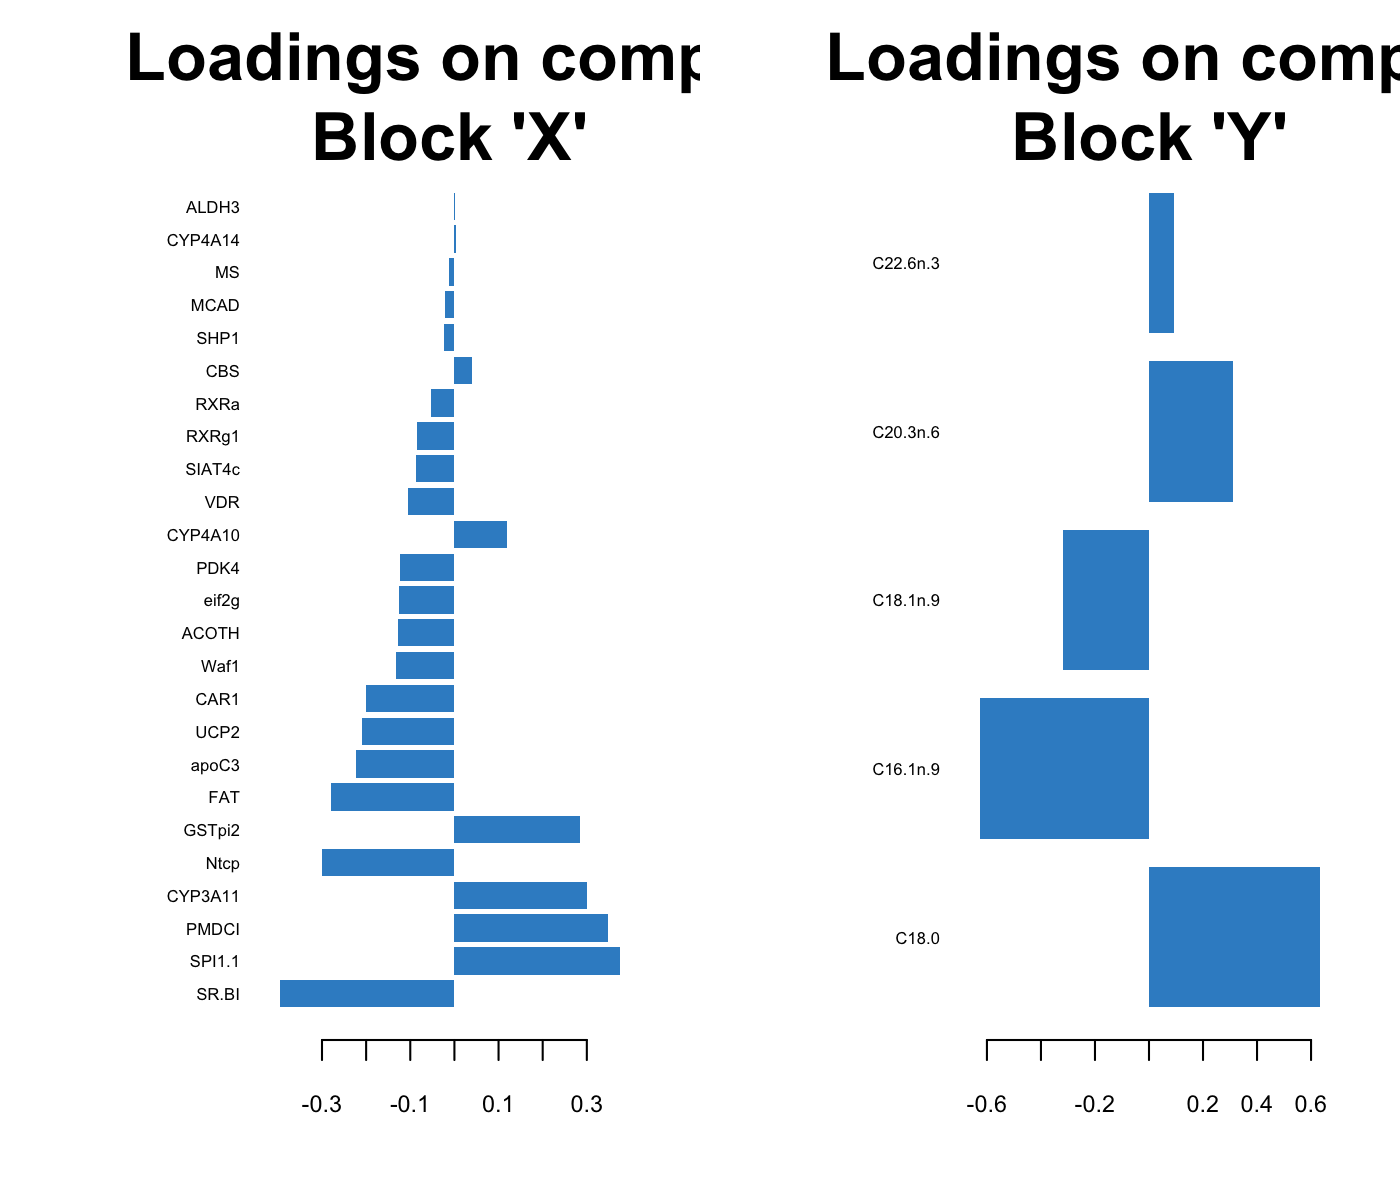
\includegraphics[width=0.5\linewidth]{Figures/unnamed-chunk-10-1} \end{center}

\begin{Shaded}
\begin{Highlighting}[]
\KeywordTok{plotVar}\NormalTok{(MyResult.spca, }\DataTypeTok{cex =} \DecValTok{1}\NormalTok{)                                        }\CommentTok{# 3 Plot the variables}
\end{Highlighting}
\end{Shaded}

\begin{center}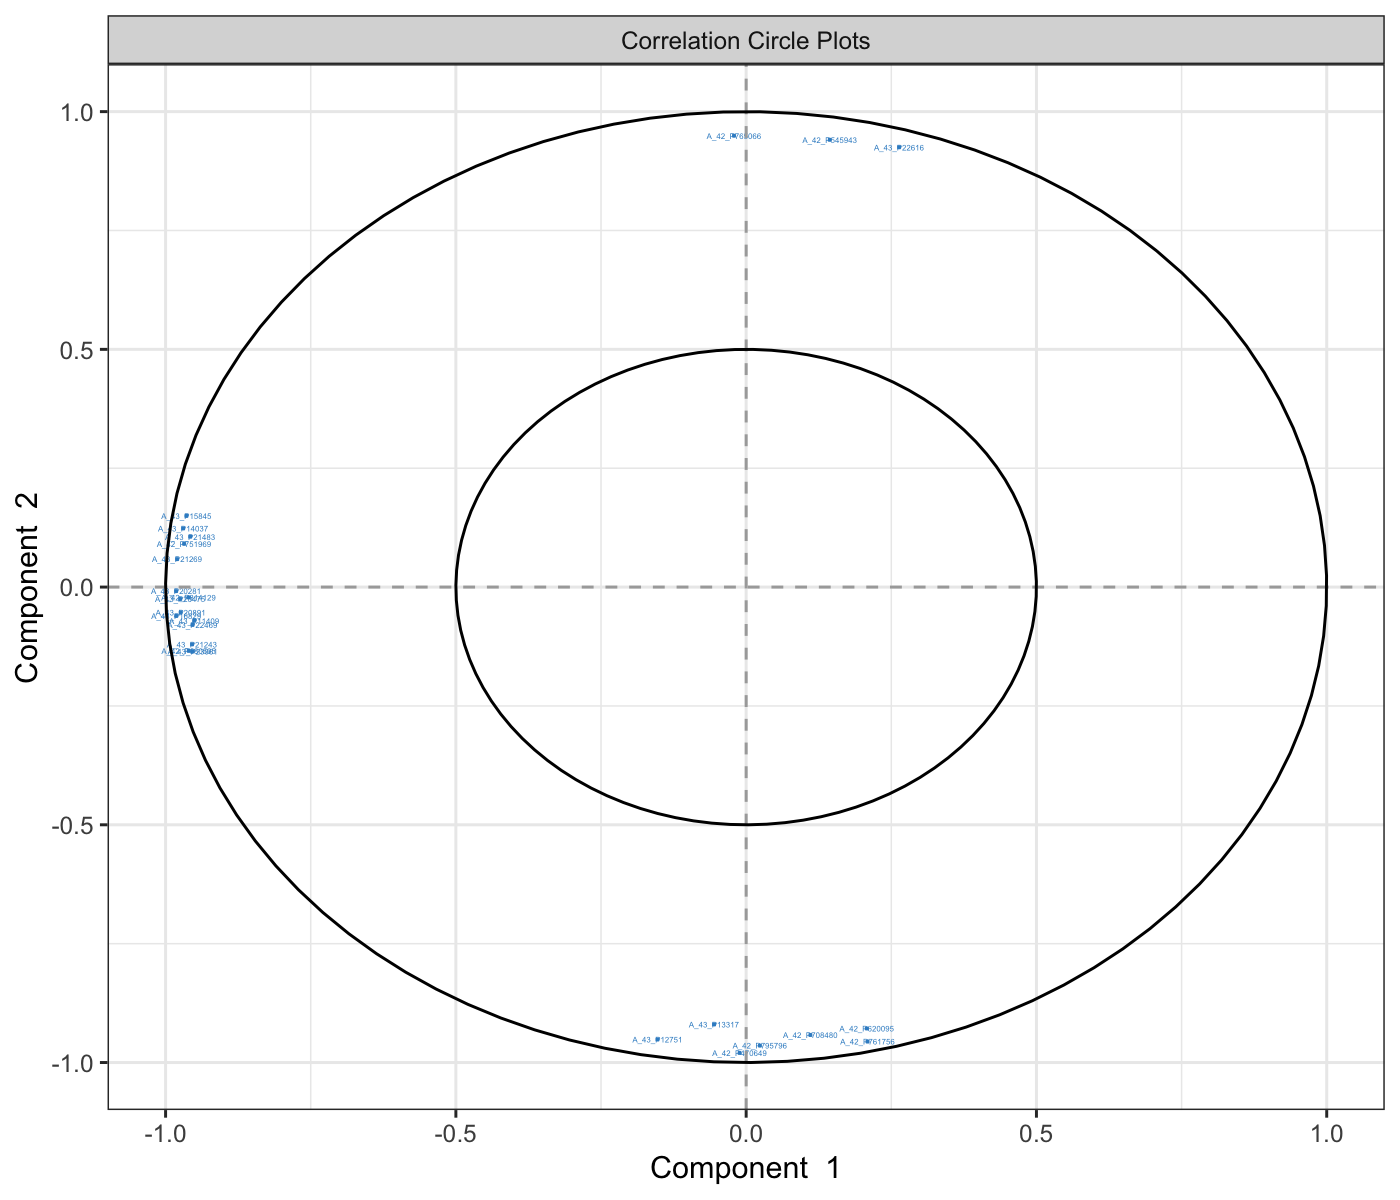
\includegraphics[width=0.5\linewidth]{Figures/unnamed-chunk-10-2} \end{center}

\begin{Shaded}
\begin{Highlighting}[]
\CommentTok{# cex is used to reduce the size of the labels on the plot}
\end{Highlighting}
\end{Shaded}

Selected variables can be identified on each component with the
\texttt{selectVar} function. Here the coefficient values are extracted,
but there are other outputs, see \texttt{?selectVar}:

\begin{Shaded}
\begin{Highlighting}[]
\KeywordTok{selectVar}\NormalTok{(MyResult.spca, }\DataTypeTok{comp =} \DecValTok{1}\NormalTok{)}\OperatorTok{$}\NormalTok{value}
\end{Highlighting}
\end{Shaded}

\begin{verbatim}
##                value.var
## A_43_P20281  -0.39077443
## A_43_P16829  -0.38898291
## A_43_P21269  -0.37452039
## A_43_P20475  -0.32482960
## A_43_P20891  -0.31740002
## A_43_P14037  -0.27681845
## A_42_P751969 -0.26140533
## A_43_P15845  -0.22392912
## A_42_P814129 -0.18838954
## A_42_P680505 -0.18672610
## A_43_P21483  -0.16202222
## A_43_P21243  -0.13259471
## A_43_P22469  -0.12493156
## A_43_P23061  -0.12255308
## A_43_P11409  -0.09768656
\end{verbatim}

Those values correspond to the loading weights that are used to define
each component. A large absolute value indicates the importance of the
variable in this PC. Selected variables are ranked from the most
important (top) to the least important.

We can complement this output with \texttt{plotLoadings}. We can see
here that all coefficients are negative.

\begin{Shaded}
\begin{Highlighting}[]
\KeywordTok{plotLoadings}\NormalTok{(MyResult.spca)}
\end{Highlighting}
\end{Shaded}

\begin{center}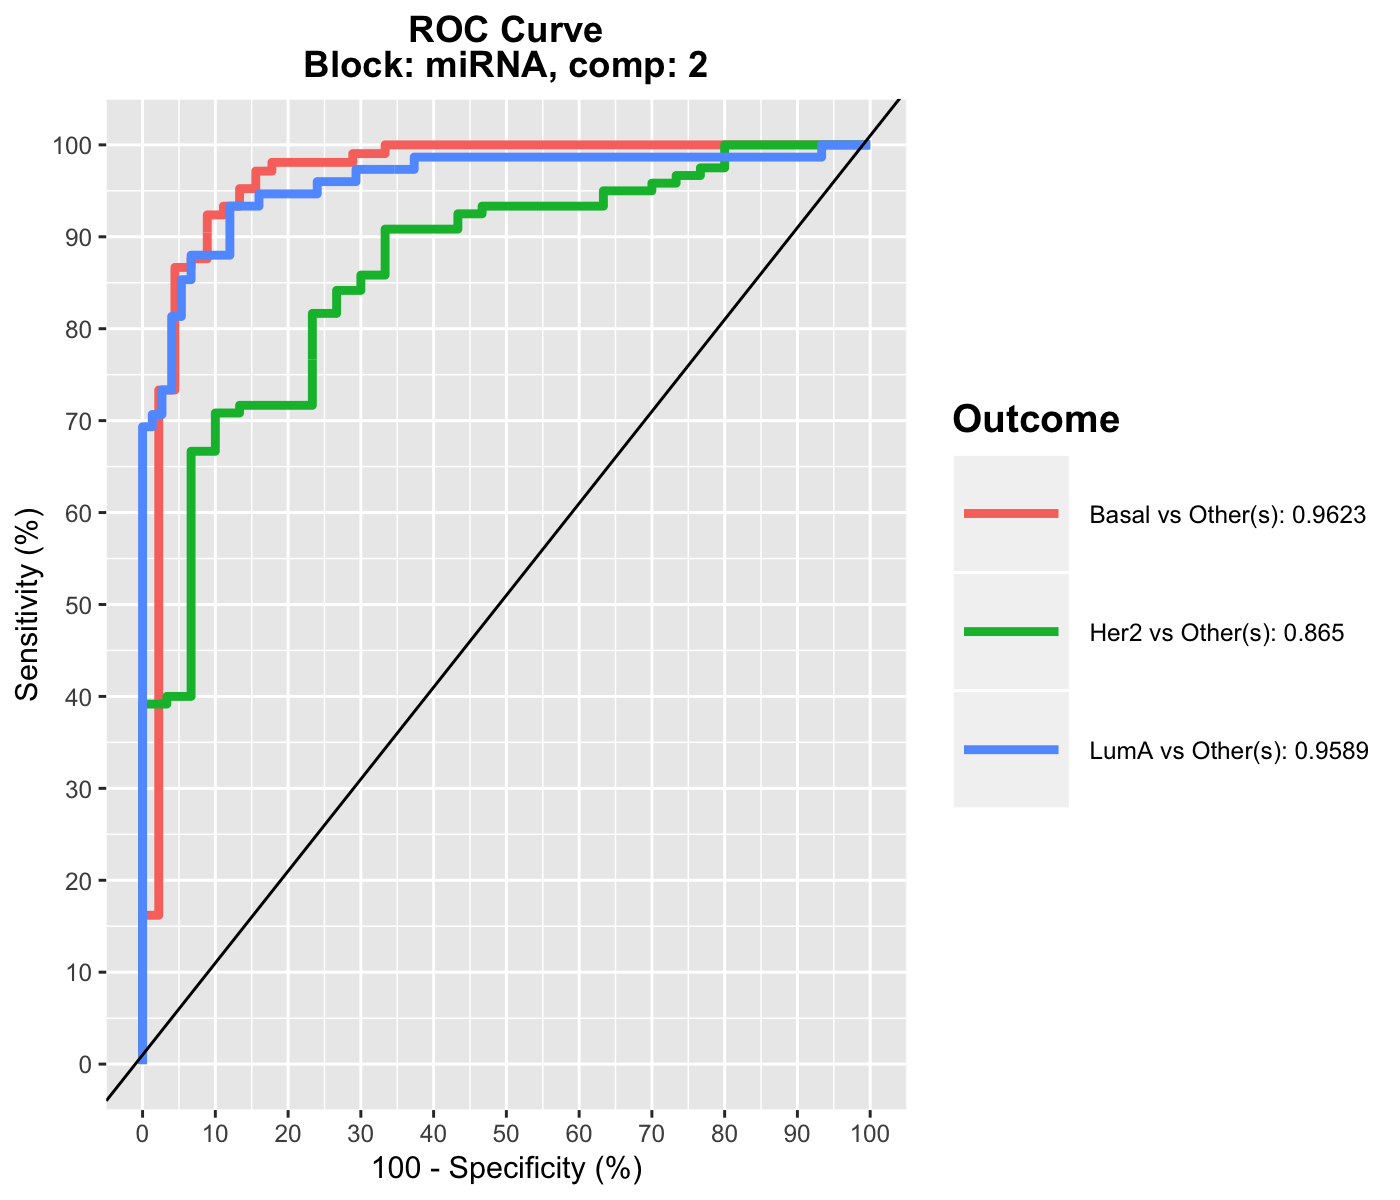
\includegraphics[width=0.5\linewidth]{Figures/unnamed-chunk-12-1} \end{center}

If we look at component two, we can see a mix of positive and negative
weights (also see in the \texttt{plotVar}), those correspond to
variables that oppose the low and high doses (see from the `plotIndiv):

\begin{center}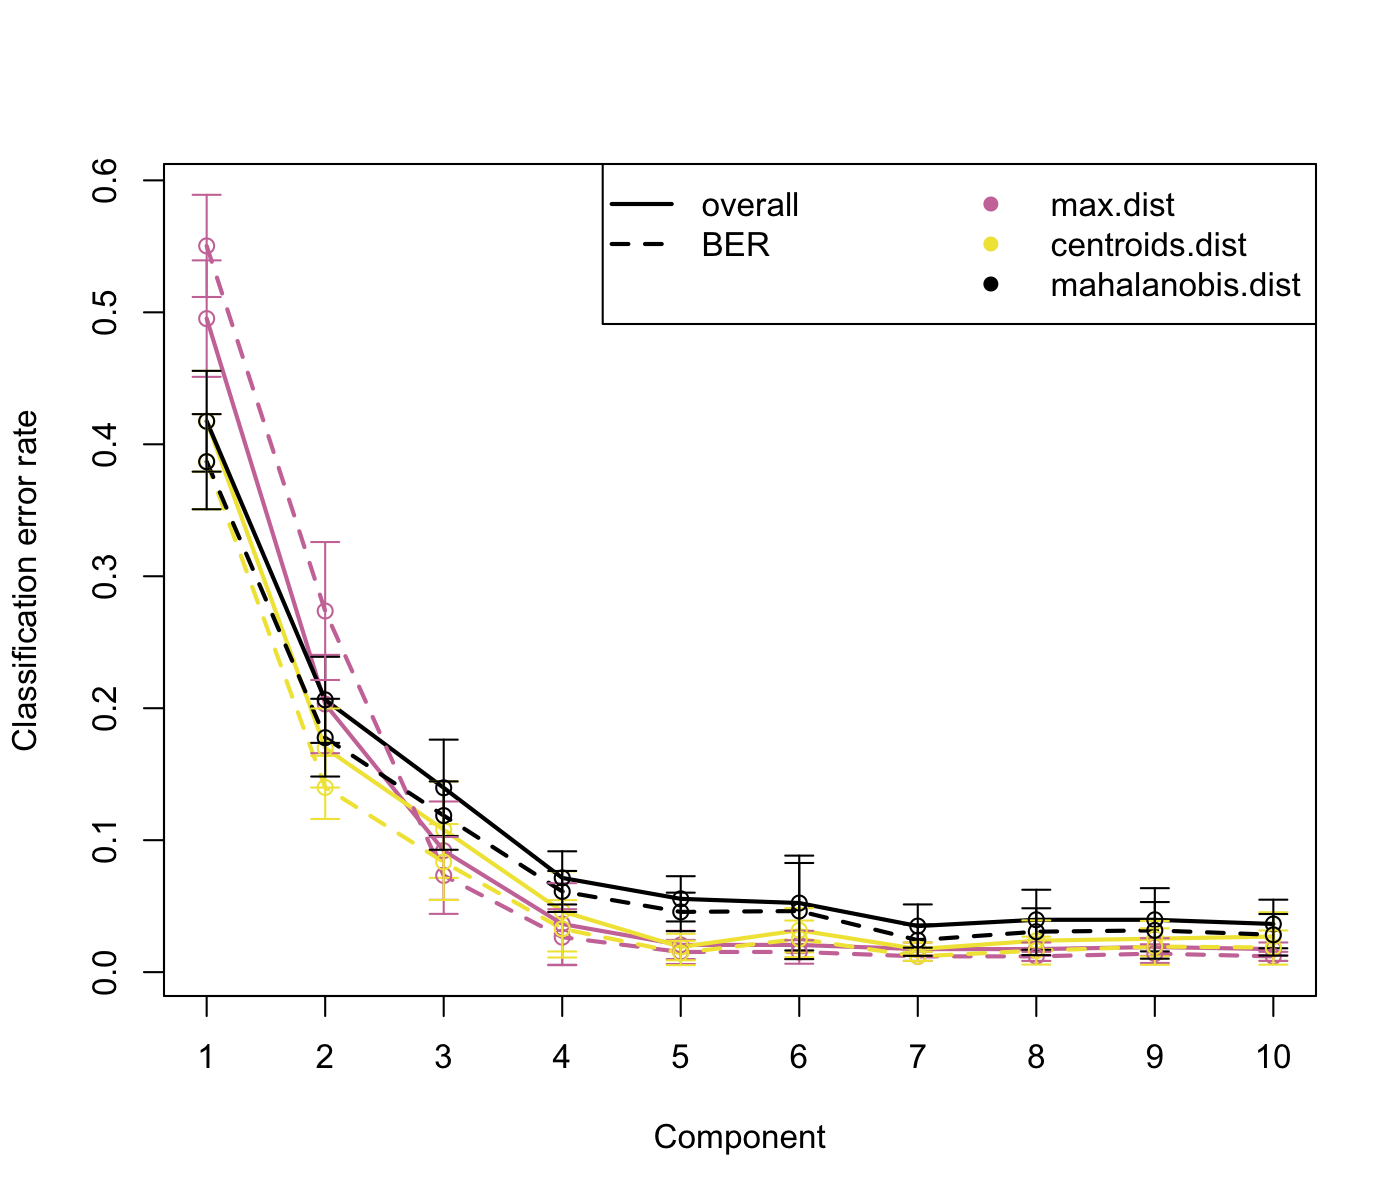
\includegraphics[width=0.5\linewidth]{Figures/unnamed-chunk-13-1} \end{center}

\section{Tuning parameters}\label{tuning-parameters}

For this set of methods, two parameters need to be chosen:

\begin{itemize}
\tightlist
\item
  The number of components to retain,
\item
  The number of variables to select on each component for sparse PCA.
\end{itemize}

The function \texttt{tune.pca} calculates the percentage of variance
explained for each component, up to the minimum between the number of
rows, or column in the data set. The `optimal' number of components can
be identified if an elbow appears on the screeplot. In the example below
the cut-off is not very clear, we could choose 2 components.

\begin{center}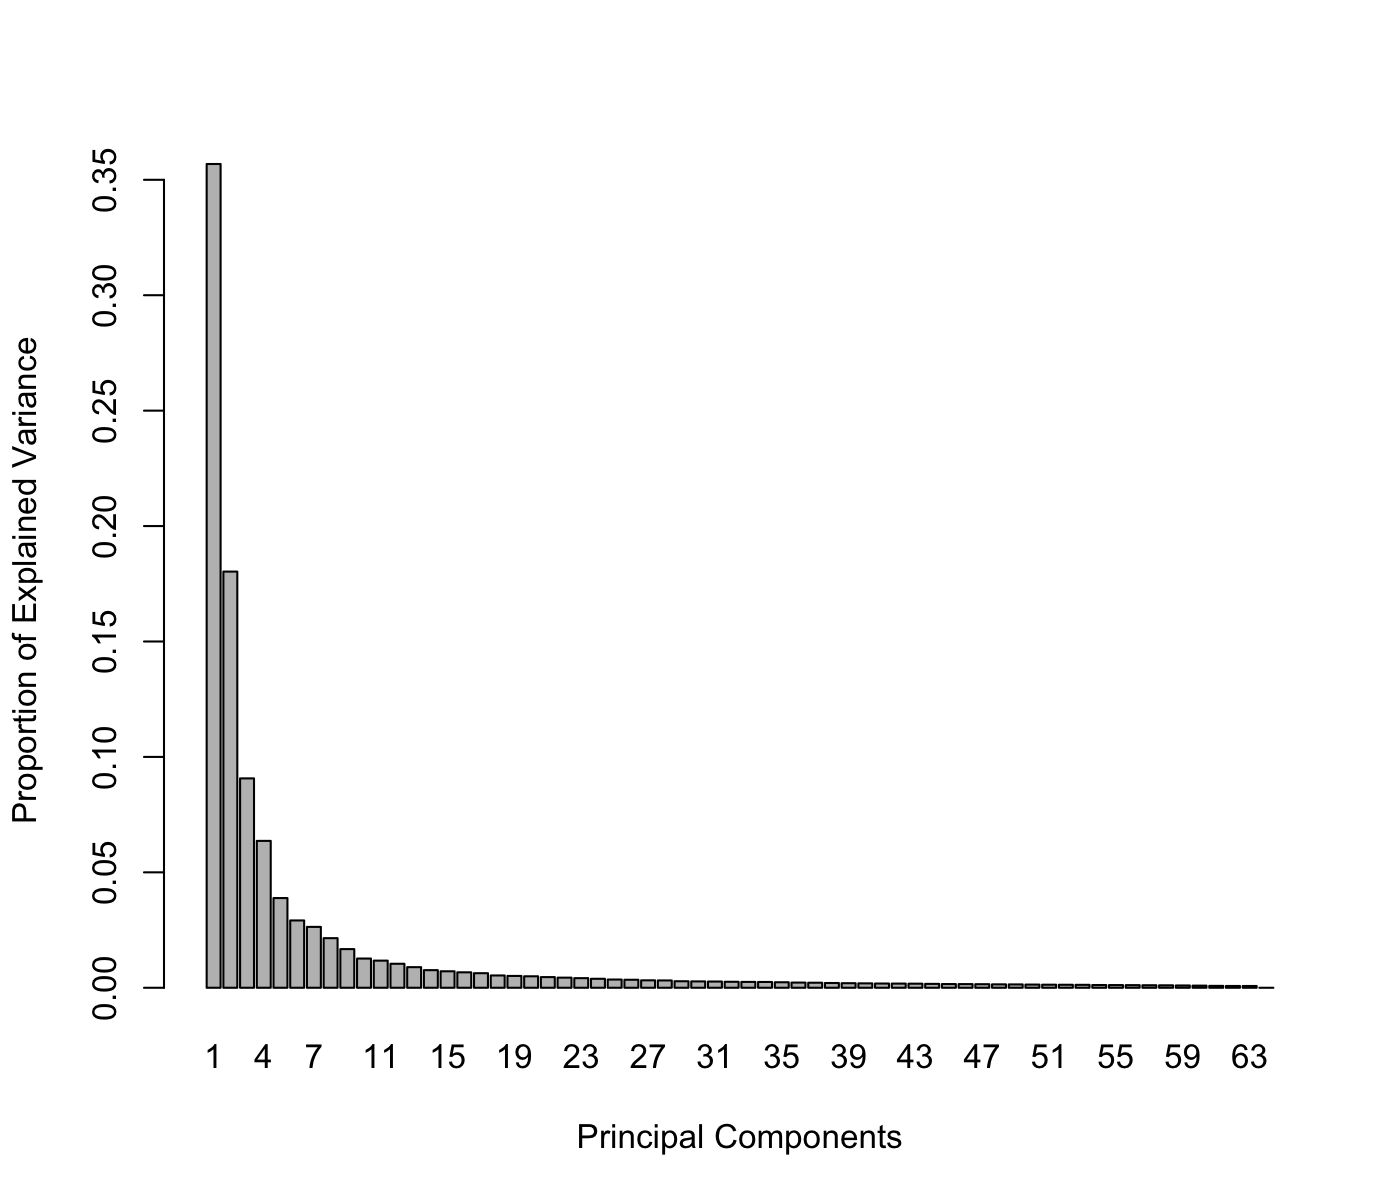
\includegraphics[width=0.5\linewidth]{Figures/unnamed-chunk-14-1} \end{center}

Regarding the number of variables to select in sparse PCA, there is not
clear criterion at this stage. As PCA is an exploration method, we
prefer to set arbitrary thresholds that will pinpoint the key variables
to focus on during the interpretation stage.

\section{Additional resources}\label{additional-resources}

Additional examples are provided in \texttt{example(pca)} and in our
case studies on our \href{http://www.mixomics.org}{website} in the
\textbf{Methods} and \textbf{Case studies} sections.

Additional reading in \citep{She08}.

\section{FAQ}\label{faq}

\begin{itemize}
\tightlist
\item
  Should I scale my data before running PCA? (\texttt{scale\ =\ TRUE} in
  \texttt{pca})

  \begin{itemize}
  \tightlist
  \item
    Without scaling: a variable with high variance will solely drive the
    first principal component
  \item
    With scaling: one noisy variable with low variability will be
    assigned the same variance as other meaningful variables
  \end{itemize}
\item
  Can I perform PCA with missing values?

  \begin{itemize}
  \tightlist
  \item
    NIPALS ( Non-linear Iterative PArtial Least Squares - implemented in
    mixOmics ) can impute missing values but must be built on many
    components. The proportion of NAs should not exceed 20\% of total
    data.
  \end{itemize}
\item
  When should I apply a multilevel approach in PCA? (\texttt{multilevel}
  argument in \texttt{PCA})

  \begin{itemize}
  \tightlist
  \item
    When the unique individuals are measured more than once (repeated
    measures)
  \item
    When the individual variation is less than treatment or time
    variation. This means that samples from each unique individual will
    tend to cluster rather than the treatments.
  \item
    When a multilevel vs no multilevel seems to visually make a
    difference on a PCA plot
  \item
    More details in this
    \href{http://mixomics.org/case-studies/multilevel-vac18/}{case
    study}
  \end{itemize}
\item
  When should I apply a CLR transformation in PCA?
  (\texttt{logratio\ =\ \textquotesingle{}CLR\textquotesingle{}}
  argument in \texttt{PCA})

  \begin{itemize}
  \tightlist
  \item
    When data are compositional, i.e.~expressed as relative proportions.
    This is usually the case with microbiome studies as a result of
    pre-processing and normalisation, see more details
    \href{http://mixomics.org/mixmc/}{here} and in our case studies in
    the same tab.
  \end{itemize}
\end{itemize}

\chapter{PLS - Discriminant Analysis (PLS-DA)}\label{plsda}

\begin{center}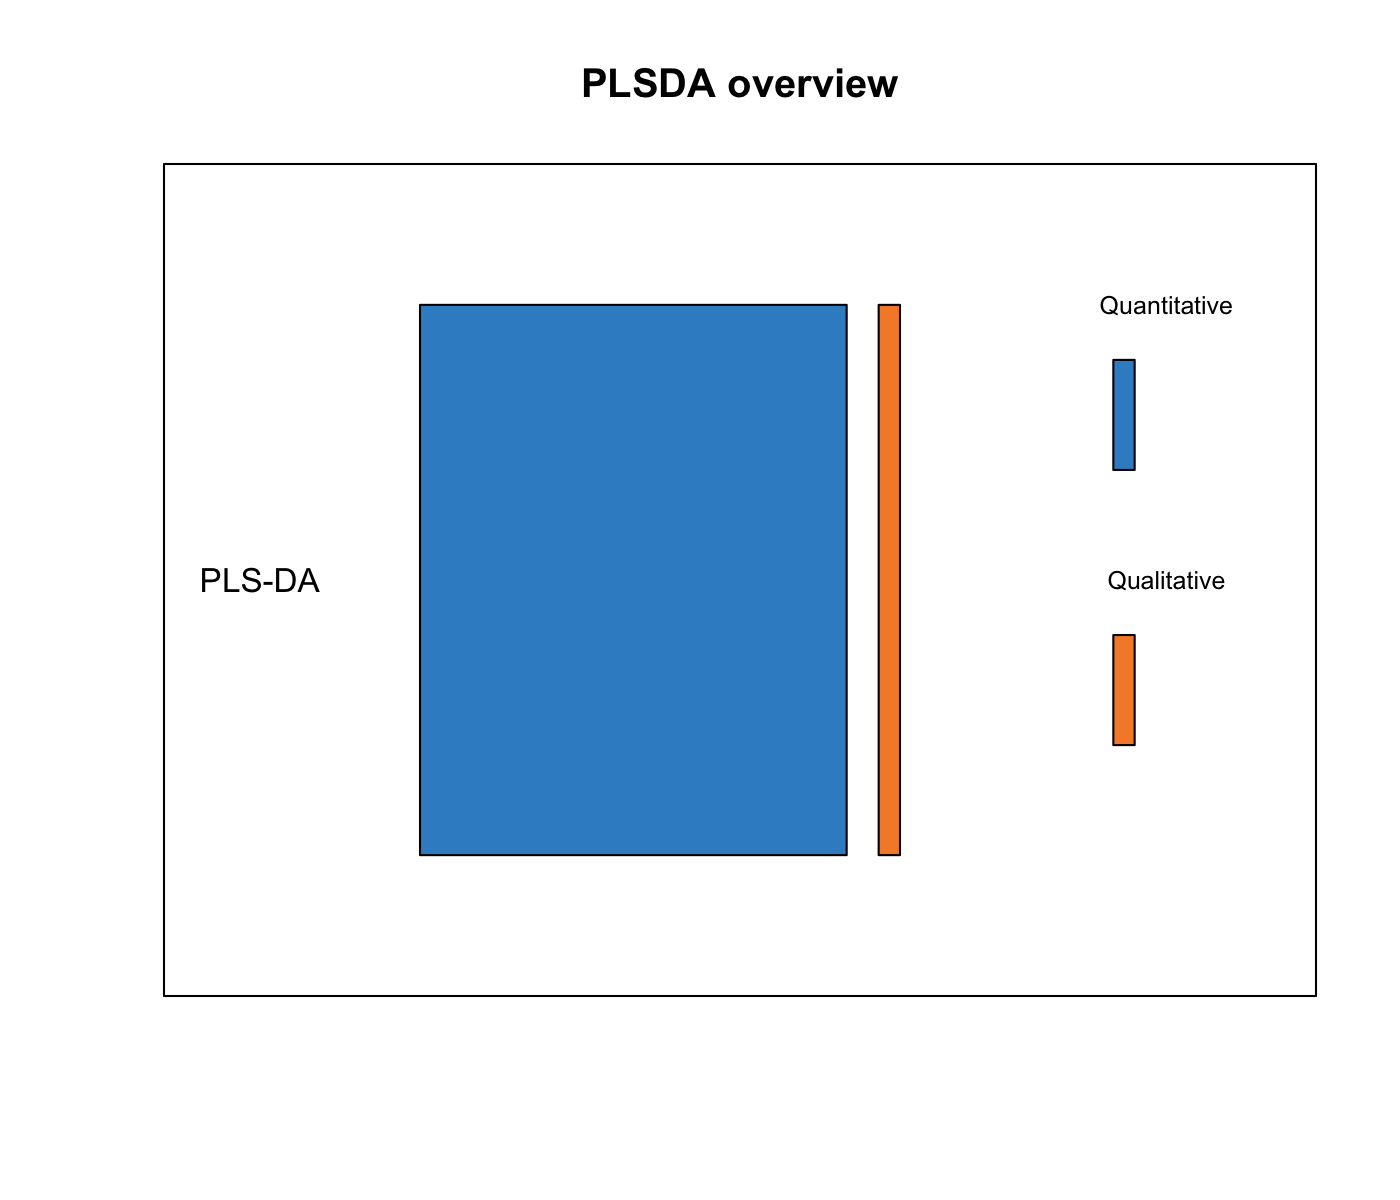
\includegraphics[width=0.5\linewidth]{Figures/overview-PLSDA-1} \end{center}

\section{Biological question}\label{biological-question-2}

{ \emph{I am analysing a single data set (e.g.~transcriptomics data) and
I would like to classify my samples into known groups and predict the
class of new samples. In addition, I am interested in identifying the
key variables that drive such discrimination.} }

\section{\texorpdfstring{The \texttt{srbct}
study}{The srbct study}}\label{the-srbct-study}

The data are directly available in a processed and normalised format
from the package. The Small Round Blue Cell Tumours (SRBCT) dataset from
\citep{Kha01} includes the expression levels of 2,308 genes measured on
63 samples. The samples are classified into four classes as follows: 8
Burkitt Lymphoma (BL), 23 Ewing Sarcoma (EWS), 12 neuroblastoma (NB),
and 20 rhabdomyosarcoma (RMS).

The srbct dataset contains the following:

\textbf{\$gene:} a data frame with 63 rows and 2308 columns. The
expression levels of 2,308 genes in 63 subjects.

\textbf{\$class:} a class vector containing the class tumour of each
individual (4 classes in total).

\textbf{\$gene.name:} a data frame with 2,308 rows and 2 columns
containing further information on the genes.

More details can be found in \texttt{?srbct}.

To illustrate PLS-DA, we will analyse the gene expression levels of
\texttt{srbct\$gene} to discriminate the 4 groups of tumours.

\section{Principle of sparse PLS-DA}\label{principle-of-sparse-pls-da}

Although Partial Least Squares was not originally designed for
classification and discrimination problems, it has often been used for
that purpose \citep{Ngu02a, Tan04}. The response matrix \texttt{Y} is
qualitative and is internally recoded as a dummy block matrix that
records the membership of each observation, i.e.~each of the response
categories are coded via an indicator variable (see \citep{mixomics}
Suppl. Information S1 for an illustration). The PLS regression (now
PLS-DA) is then run as if Y was a continuous matrix. This PLS
classification trick works well in practice, as demonstrated in many
references \citep{Bar03, Ngu02a, Bou07, Chung10}.

Sparse PLS-DA \citep{Lec11} performs variable selection and
classification in a one step procedure. sPLS-DA is a special case of
sparse PLS described later in \ref{pls}, where \(\ell_1\) penalization
is applied on the loading vectors associated to the X data set.

\section{Inputs and outputs}\label{inputs-and-outputs}

We use the following data input matrices: \texttt{X} is a \(n \times p\)
data matrix, \texttt{Y} is a factor vector of length \(n\) that
indicates the class of each sample, and \(Y^*\) is the associated dummy
matrix (\(n \times K\)) with \(n\) the number of samples (individuals),
\(p\) the number of variables and \(K\) the number of classes. PLS-DA
main outputs are:

\begin{itemize}
\item
  A \textbf{set of components}, also called latent variables. There are
  as many components as the chosen \emph{dimension} of the PLS-DA model.
\item
  A \textbf{set of loading vectors}, which are coefficients assigned to
  each variable to define each component. Those coefficients indicate
  the importance of each variable in PLS-DA. Importantly, each loading
  vector is associated to a particular component. Loading vectors are
  obtained so that the covariance between a linear combination of the
  variables from X (the X-component) and the factor of interest Y (the
  \(Y^*\)-component) is maximised.
\item
  A \textbf{list of selected variables} from \texttt{X} and associated
  to each component if sPLS-DA is applied.
\end{itemize}

\section{Set up the data}\label{set-up-the-data}

We first load the data from the package. See \ref{start:upload} to
upload your own data.

We will mainly focus on sparse PLS-DA that is more suited for large
biological data sets where the aim is to identify molecular signatures,
as well as classifying samples. We first set up the data as \texttt{X}
expression matrix and \texttt{Y} as a factor indicating the class
membership of each sample. We also check that the dimensions are correct
and match:

\begin{Shaded}
\begin{Highlighting}[]
\KeywordTok{library}\NormalTok{(mixOmics)}
\KeywordTok{data}\NormalTok{(srbct)}
\NormalTok{X <-}\StringTok{ }\NormalTok{srbct}\OperatorTok{$}\NormalTok{gene}
\NormalTok{Y <-}\StringTok{ }\NormalTok{srbct}\OperatorTok{$}\NormalTok{class }
\KeywordTok{summary}\NormalTok{(Y)}
\end{Highlighting}
\end{Shaded}

\begin{verbatim}
## EWS  BL  NB RMS 
##  23   8  12  20
\end{verbatim}

\begin{Shaded}
\begin{Highlighting}[]
\KeywordTok{dim}\NormalTok{(X); }\KeywordTok{length}\NormalTok{(Y)}
\end{Highlighting}
\end{Shaded}

\begin{verbatim}
## [1]   63 2308
\end{verbatim}

\begin{verbatim}
## [1] 63
\end{verbatim}

\section{Quick start}\label{quick-start-1}

For a quick start we arbitrarily set the number of variables to select
to 50 on each of the 3 components of PLS-DA (see section
\ref{tuning:sPLSDA} for tuning these values).

As PLS-DA is a supervised method, the sample plot automatically displays
the group membership of each sample. We can observe a clear
discrimination between the BL samples and the others on the first
component (x-axis), and EWS vs the others on the second component
(y-axis). Remember that this discrimination spanned by the first two
PLS-DA components is obtained based on a subset of 100 variables (50
selected on each component).

From the \texttt{plotIndiv} the axis labels indicate the amount of
variation explained per component. Note that the interpretation of this
amount is \emph{not} the same as in PCA. In PLS-DA, the aim is to
maximise the covariance between \texttt{X} and \texttt{Y}, not only the
variance of \texttt{X} as it is the case in PCA!

If you were to run \texttt{splsda} with this minimal code, you would be
using the following default values:

\begin{itemize}
\tightlist
\item
  \texttt{ncomp\ =\ 2}: the first two PLS components are calculated and
  are used for graphical outputs;
\item
  \texttt{scale\ =\ TRUE}: data are scaled (variance = 1, strongly
  advised here);
\item
  \texttt{mode\ =\ "regression"}: by default a PLS regression mode
  should be used.
\end{itemize}

PLS-DA without variable selection can be performed as:

\begin{Shaded}
\begin{Highlighting}[]
\NormalTok{MyResult.plsda <-}\StringTok{ }\KeywordTok{plsda}\NormalTok{(X,Y) }\CommentTok{# 1 Run the method}
\KeywordTok{plotIndiv}\NormalTok{(MyResult.plsda)    }\CommentTok{# 2 Plot the samples}
\end{Highlighting}
\end{Shaded}

\begin{Shaded}
\begin{Highlighting}[]
\KeywordTok{plotVar}\NormalTok{(MyResult.plsda)      }\CommentTok{# 3 Plot the variables}
\end{Highlighting}
\end{Shaded}

\section{To go further}\label{plsda-tgf}

\subsection{Customize sample plots}\label{splsda:plotIndiv}

The sample plots can be improved in various ways. First, if the names of
the samples are not meaningful at this stage, they can be replaced by
symbols (\texttt{ind.names=TRUE}). Confidence ellipses can be plotted
for each sample (\texttt{ellipse\ =\ TRUE}, confidence level set to 95\%
by default, see the argument \texttt{ellipse.level}), Additionally, a
star plot displays arrows from each group centroid towards each
individual sample (\texttt{star\ =\ TRUE}). A 3D plot is also available,
see \texttt{plotIndiv} for more details.

\begin{Shaded}
\begin{Highlighting}[]
\KeywordTok{plotIndiv}\NormalTok{(MyResult.splsda, }\DataTypeTok{ind.names =} \OtherTok{FALSE}\NormalTok{, }\DataTypeTok{legend=}\OtherTok{TRUE}\NormalTok{,}
          \DataTypeTok{ellipse =} \OtherTok{TRUE}\NormalTok{, }\DataTypeTok{star =} \OtherTok{TRUE}\NormalTok{, }\DataTypeTok{title =} \StringTok{'sPLS-DA on SRBCT'}\NormalTok{,}
          \DataTypeTok{X.label =} \StringTok{'PLS-DA 1'}\NormalTok{, }\DataTypeTok{Y.label =} \StringTok{'PLS-DA 2'}\NormalTok{)}
\end{Highlighting}
\end{Shaded}

\begin{center}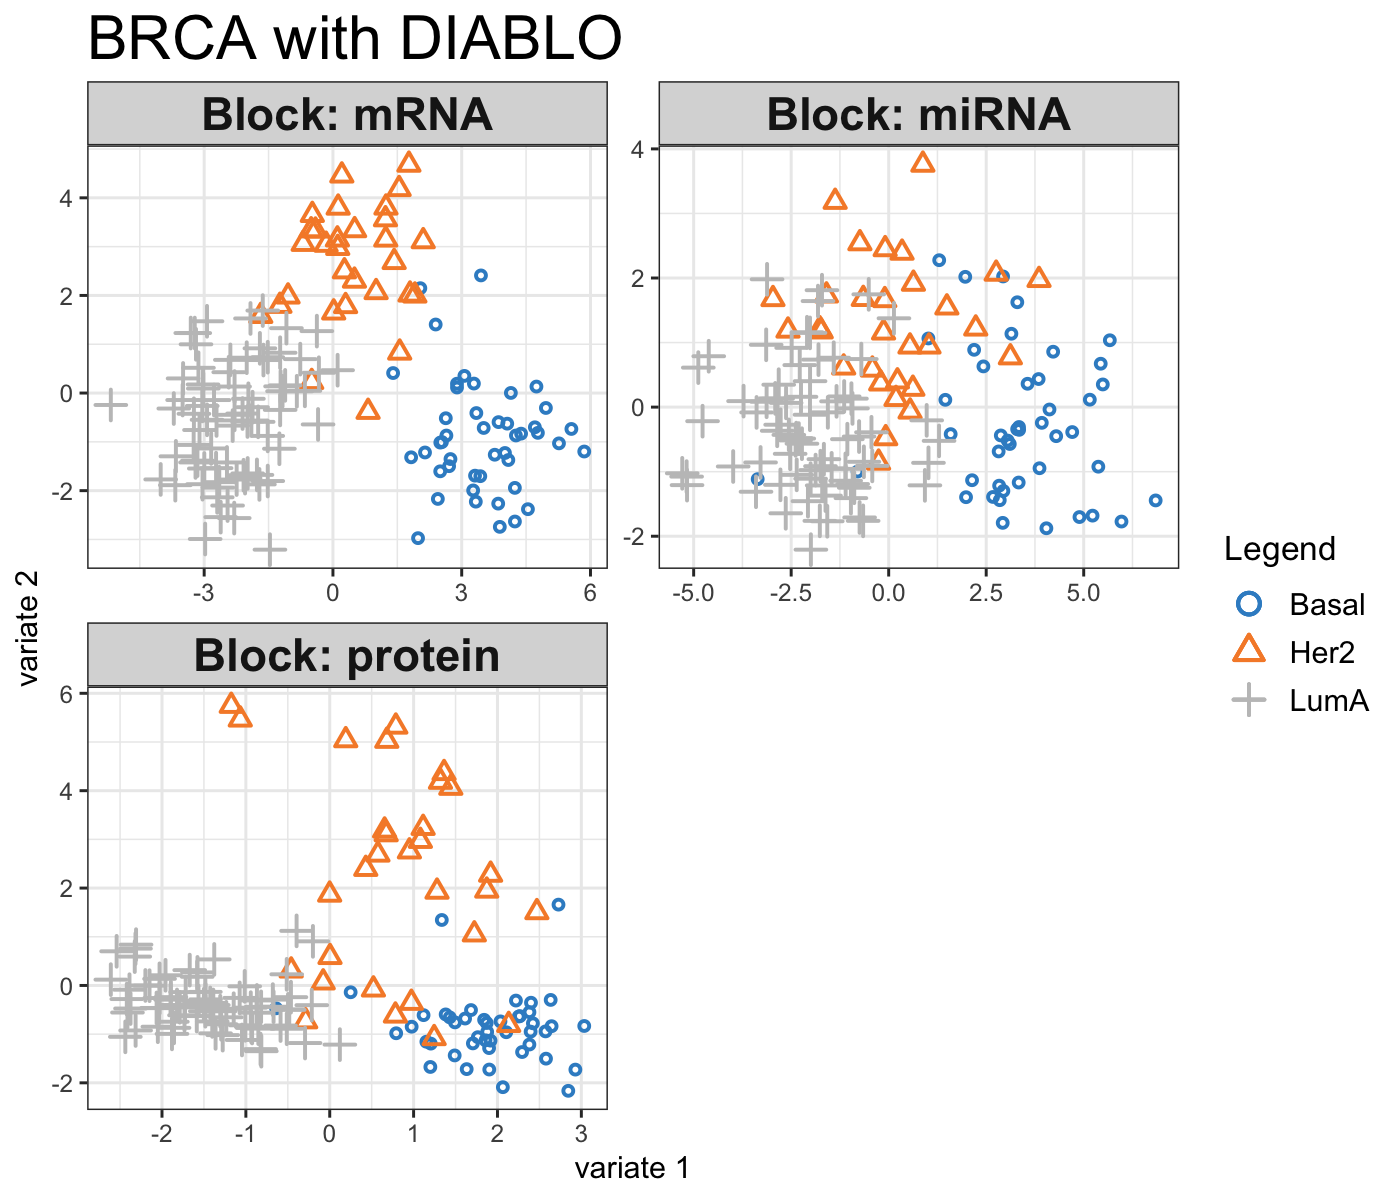
\includegraphics[width=0.5\linewidth]{Figures/unnamed-chunk-4-1} \end{center}

\subsection{Customize variable plots}\label{customize-variable-plots}

The name of the variables can be set to FALSE
(\texttt{var.names=FALSE}):

\begin{Shaded}
\begin{Highlighting}[]
\KeywordTok{plotVar}\NormalTok{(MyResult.splsda, }\DataTypeTok{var.names=}\OtherTok{FALSE}\NormalTok{)}
\end{Highlighting}
\end{Shaded}

\begin{center}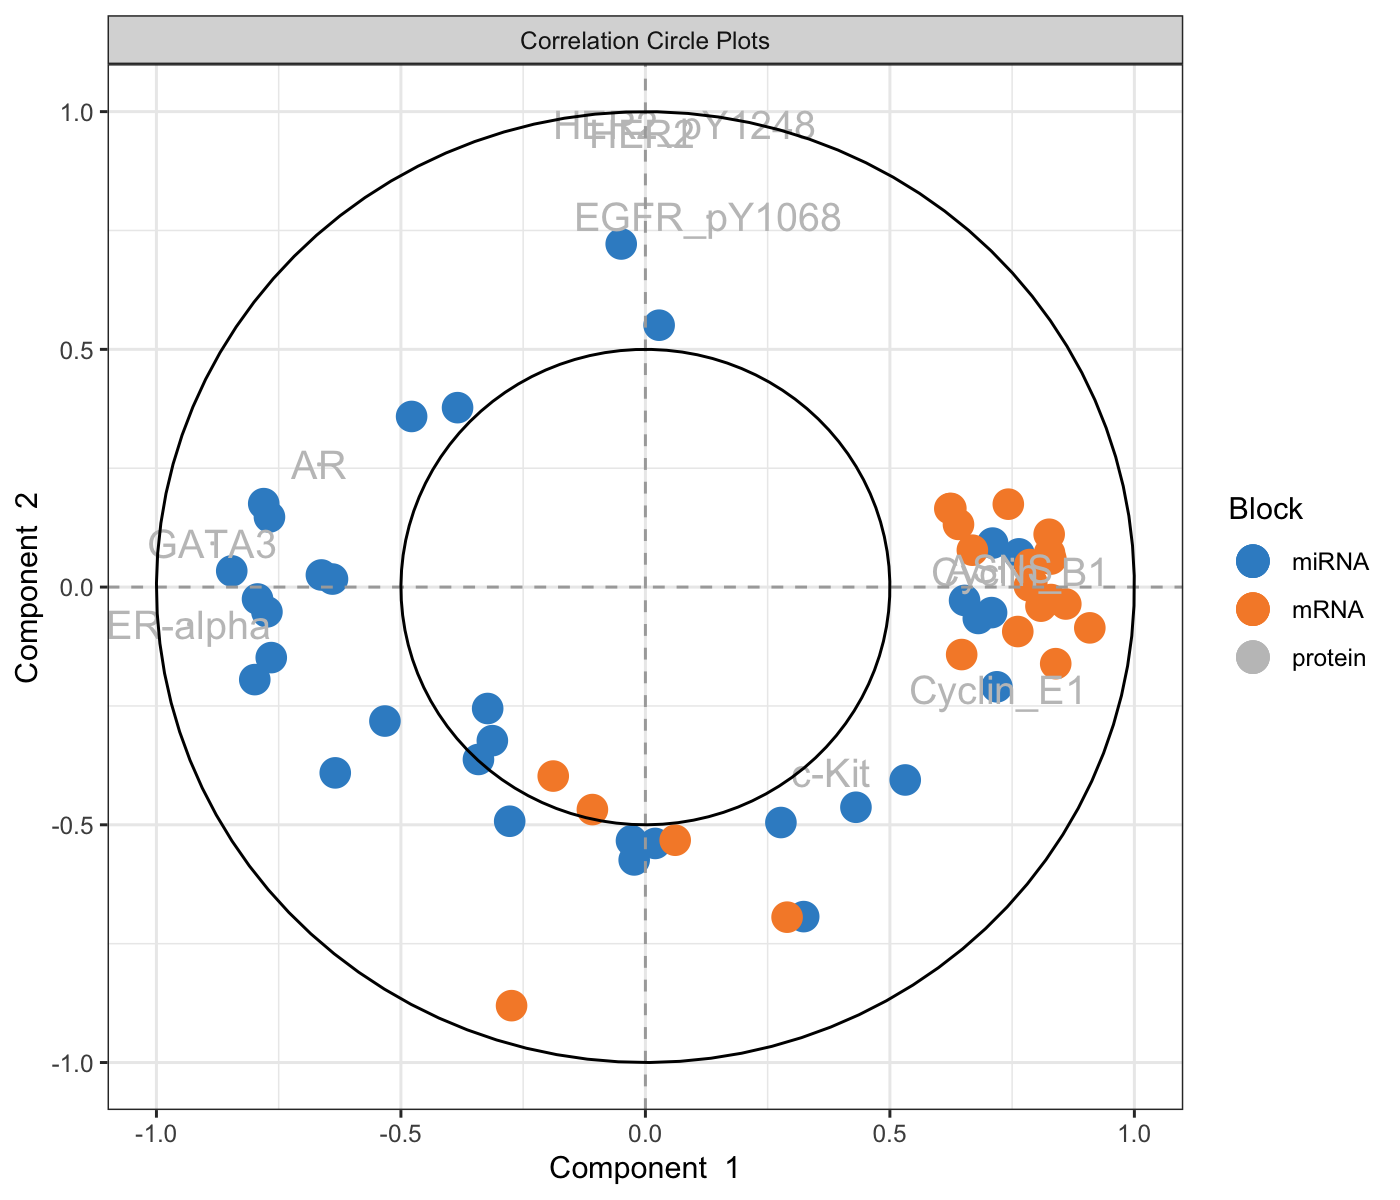
\includegraphics[width=0.5\linewidth]{Figures/unnamed-chunk-5-1} \end{center}

In addition, if we had used the non sparse version of PLS-DA, a cut-off
can be set to display only the variables that mostly contribute to the
definition of each component. Those variables should be located towards
the circle of radius 1, far from the centre.

\begin{Shaded}
\begin{Highlighting}[]
\KeywordTok{plotVar}\NormalTok{(MyResult.plsda, }\DataTypeTok{cutoff=}\FloatTok{0.7}\NormalTok{)}
\end{Highlighting}
\end{Shaded}

\begin{center}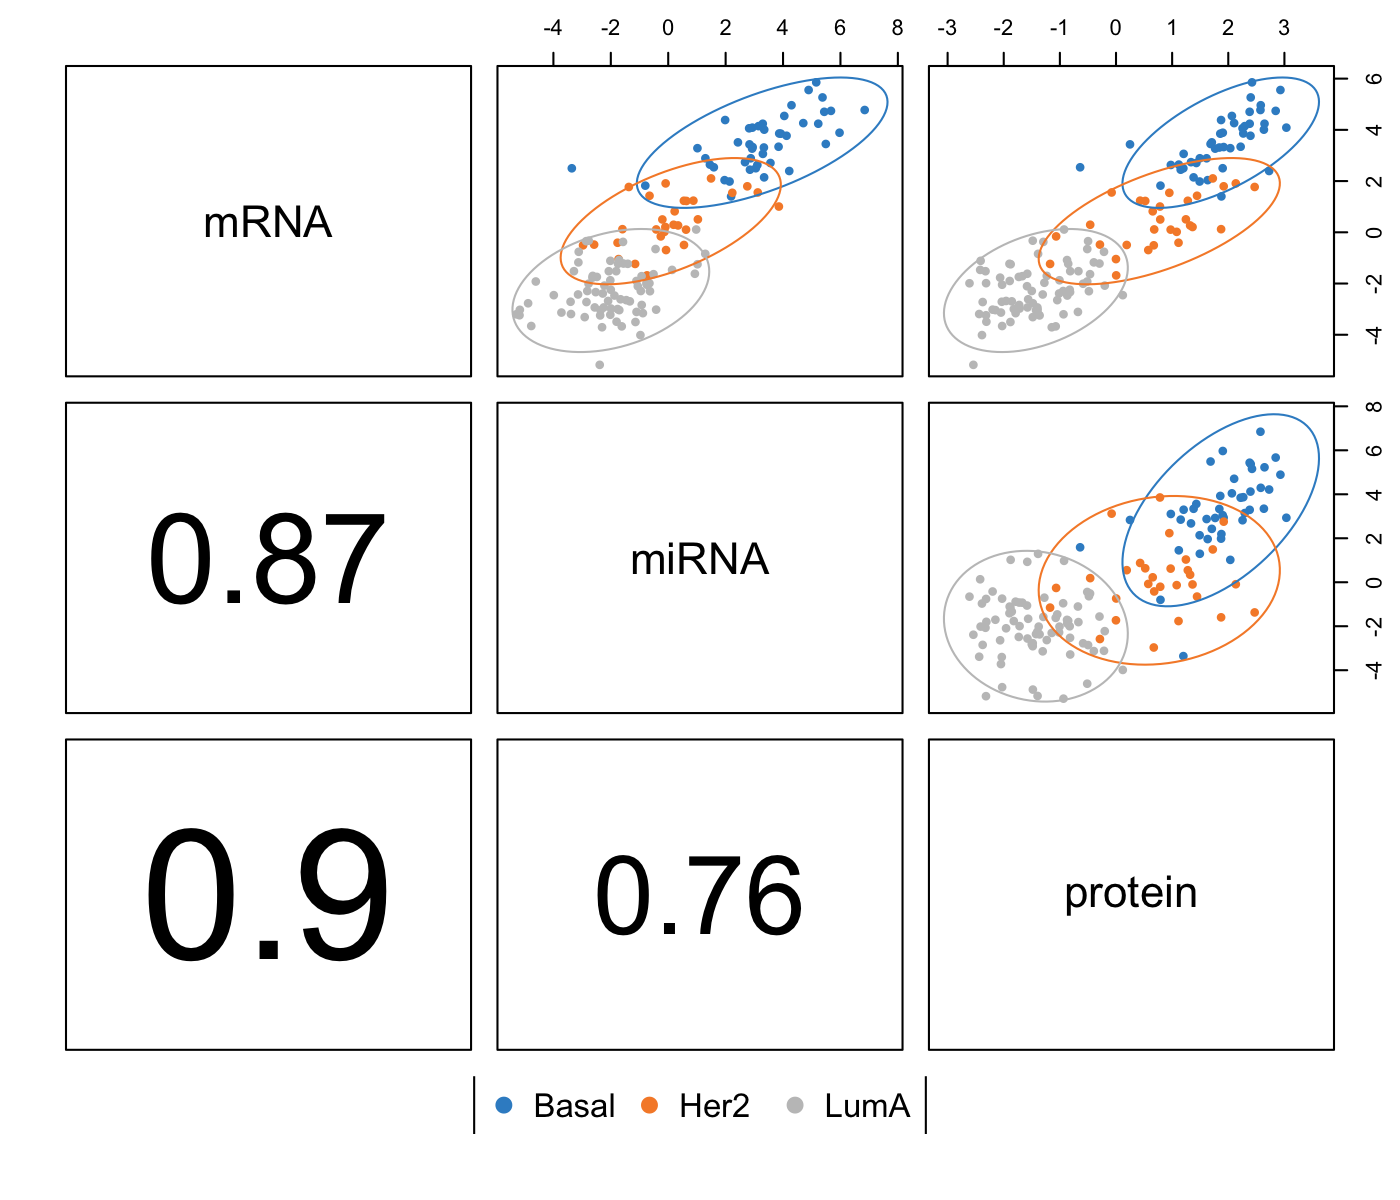
\includegraphics[width=0.5\linewidth]{Figures/unnamed-chunk-6-1} \end{center}

In this particular case, no variable selection was performed. Only the
display was altered to show a subset of variables.

\subsection{Other useful plots}\label{other-useful-plots-1}

\subsubsection{Background prediction}\label{background-prediction}

A `prediction' background can be added to the sample plot by calculating
a background surface first, before overlaying the sample plot. See
\texttt{?background.predict} for more details. More details about
prediction, prediction distances can be found in \citep{mixomics} in the
Suppl. Information.

\begin{Shaded}
\begin{Highlighting}[]
\NormalTok{background <-}\StringTok{ }\KeywordTok{background.predict}\NormalTok{(MyResult.splsda, }\DataTypeTok{comp.predicted=}\DecValTok{2}\NormalTok{,}
                                \DataTypeTok{dist =} \StringTok{"max.dist"}\NormalTok{) }
\KeywordTok{plotIndiv}\NormalTok{(MyResult.splsda, }\DataTypeTok{comp =} \DecValTok{1}\OperatorTok{:}\DecValTok{2}\NormalTok{, }\DataTypeTok{group =}\NormalTok{ srbct}\OperatorTok{$}\NormalTok{class,}
          \DataTypeTok{ind.names =} \OtherTok{FALSE}\NormalTok{, }\DataTypeTok{title =} \StringTok{"Maximum distance"}\NormalTok{,}
          \DataTypeTok{legend =} \OtherTok{TRUE}\NormalTok{,  }\DataTypeTok{background =}\NormalTok{ background)}
\end{Highlighting}
\end{Shaded}

\begin{center}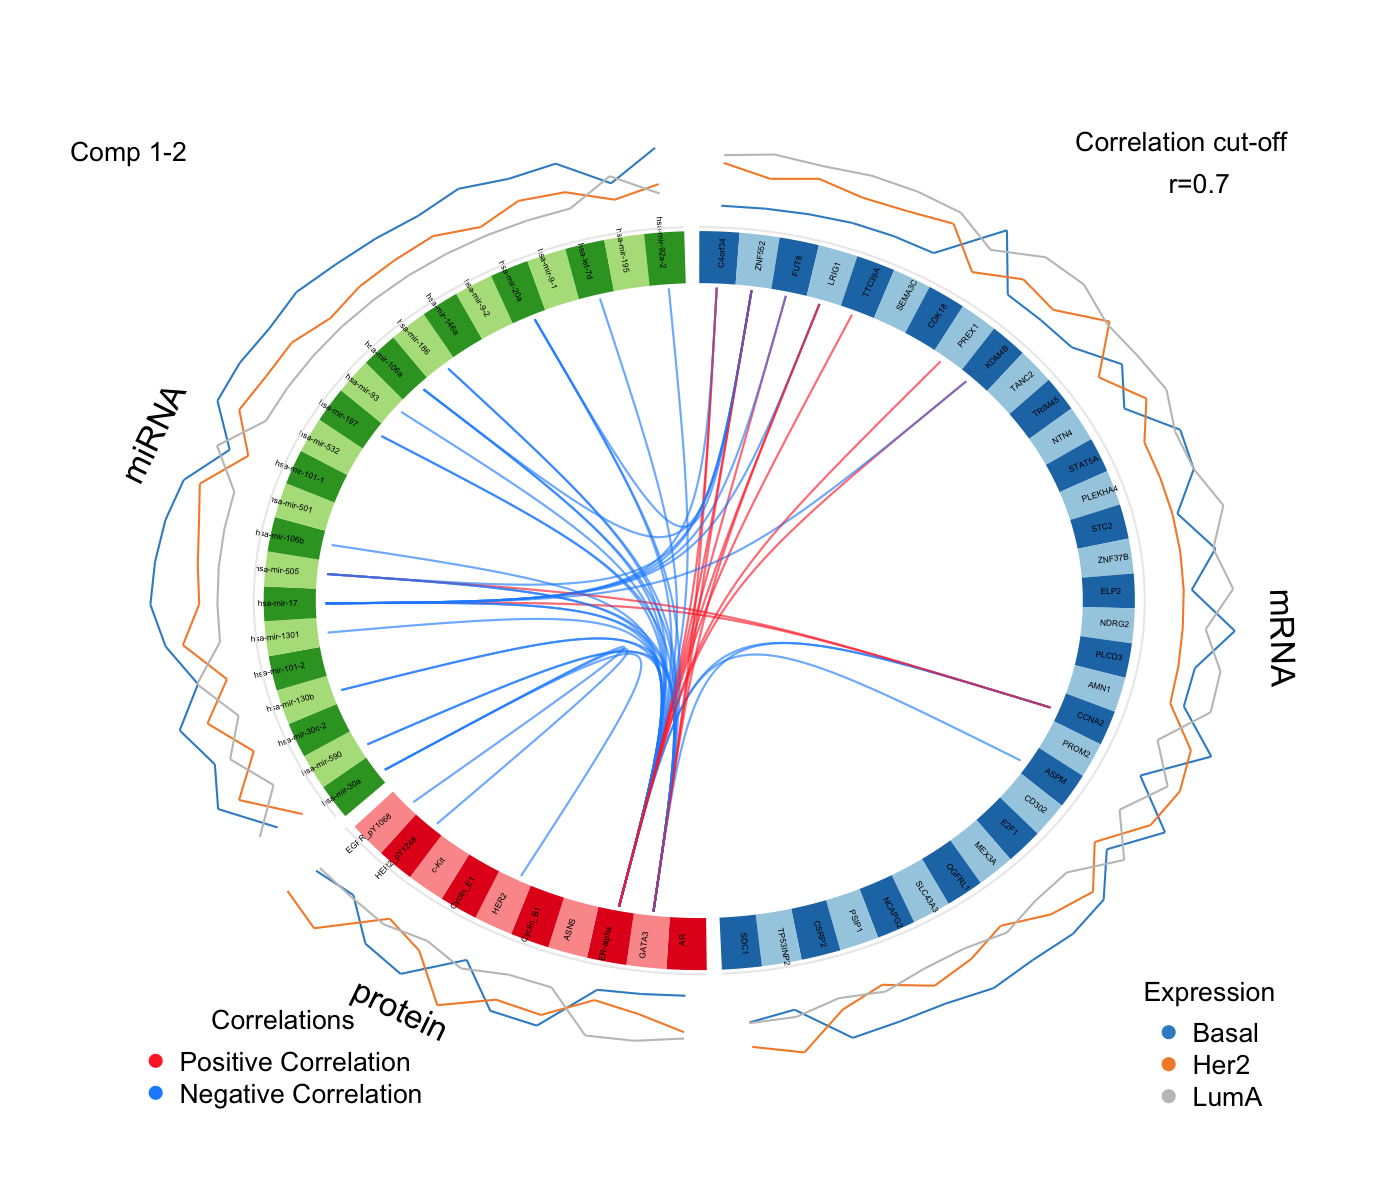
\includegraphics[width=0.5\linewidth]{Figures/unnamed-chunk-7-1} \end{center}

\subsubsection{ROC}\label{roc}

As PLS-DA acts as a classifier, we can plot a ROC Curve to complement
the sPLS-DA classification performance results detailed in
\ref{tuning:sPLSDA}. The AUC is calculated from training
cross-validation sets and averaged. Note however that ROC and AUC
criteria may not be particularly insightful, or may not be in full
agreement with the PLSDA performance, as the prediction threshold in
PLS-DA is based on specified distance as described in \citep{mixomics}.

\begin{center}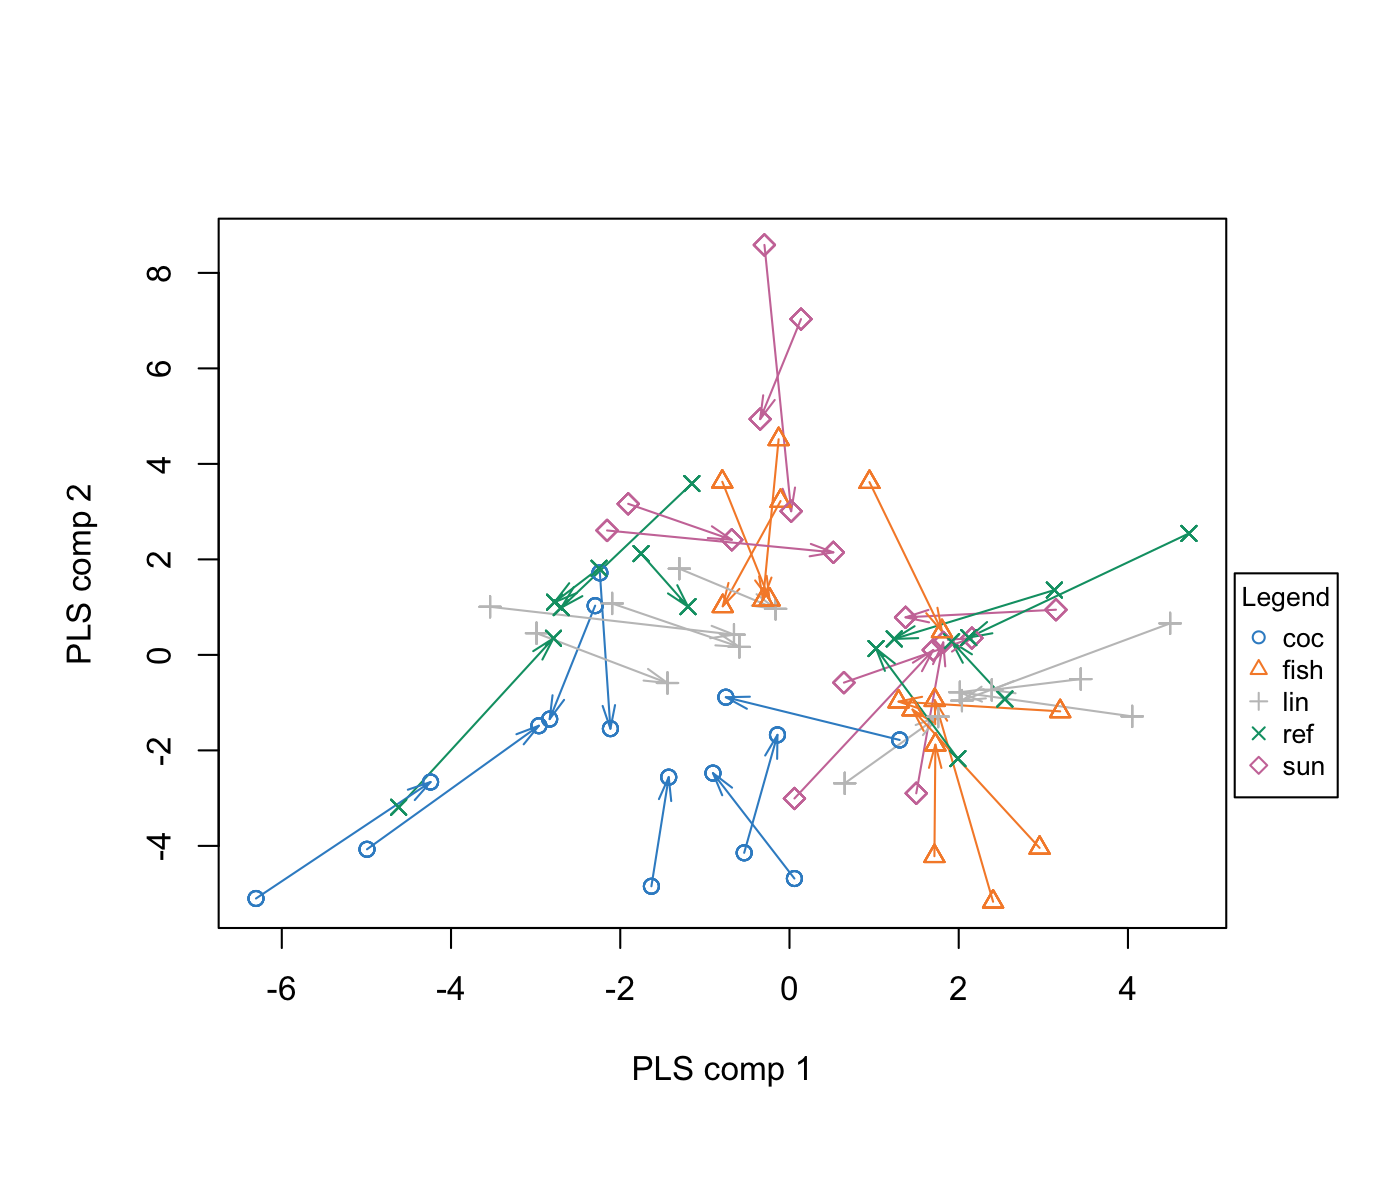
\includegraphics[width=0.5\linewidth]{Figures/unnamed-chunk-8-1} \end{center}

\subsection{Variable selection
outputs}\label{variable-selection-outputs}

First, note that the number of variables to select on each component
does not need to be identical on each component, for example:

\begin{Shaded}
\begin{Highlighting}[]
\NormalTok{MyResult.splsda2 <-}\StringTok{ }\KeywordTok{splsda}\NormalTok{(X,Y, }\DataTypeTok{ncomp=}\DecValTok{3}\NormalTok{, }\DataTypeTok{keepX=}\KeywordTok{c}\NormalTok{(}\DecValTok{15}\NormalTok{,}\DecValTok{10}\NormalTok{,}\DecValTok{5}\NormalTok{))}
\end{Highlighting}
\end{Shaded}

Selected variables are listed in the \texttt{selectVar} function:

\begin{Shaded}
\begin{Highlighting}[]
\KeywordTok{selectVar}\NormalTok{(MyResult.splsda2, }\DataTypeTok{comp=}\DecValTok{1}\NormalTok{)}\OperatorTok{$}\NormalTok{value}
\end{Highlighting}
\end{Shaded}

\begin{verbatim}
##        value.var
## g123  0.53516982
## g846  0.41271455
## g335  0.30309695
## g1606 0.30194141
## g836  0.29365241
## g783  0.26329876
## g758  0.25826903
## g1386 0.23702577
## g1158 0.15283961
## g585  0.13838913
## g589  0.12738682
## g1387 0.12202390
## g1884 0.08458869
## g1295 0.03150351
## g1036 0.00224886
\end{verbatim}

and can be visualised in \texttt{plotLoadings} with the arguments
\texttt{contrib\ =\ \textquotesingle{}max\textquotesingle{}} that is
going to assign to each variable bar the sample group colour for which
the mean (\texttt{method\ =\ \textquotesingle{}mean\textquotesingle{}})
is maximum. See \texttt{example(plotLoadings)} for other options
(e.g.~min, median)

\begin{Shaded}
\begin{Highlighting}[]
\KeywordTok{plotLoadings}\NormalTok{(MyResult.splsda2, }\DataTypeTok{contrib =} \StringTok{'max'}\NormalTok{, }\DataTypeTok{method =} \StringTok{'mean'}\NormalTok{)}
\end{Highlighting}
\end{Shaded}

\begin{center}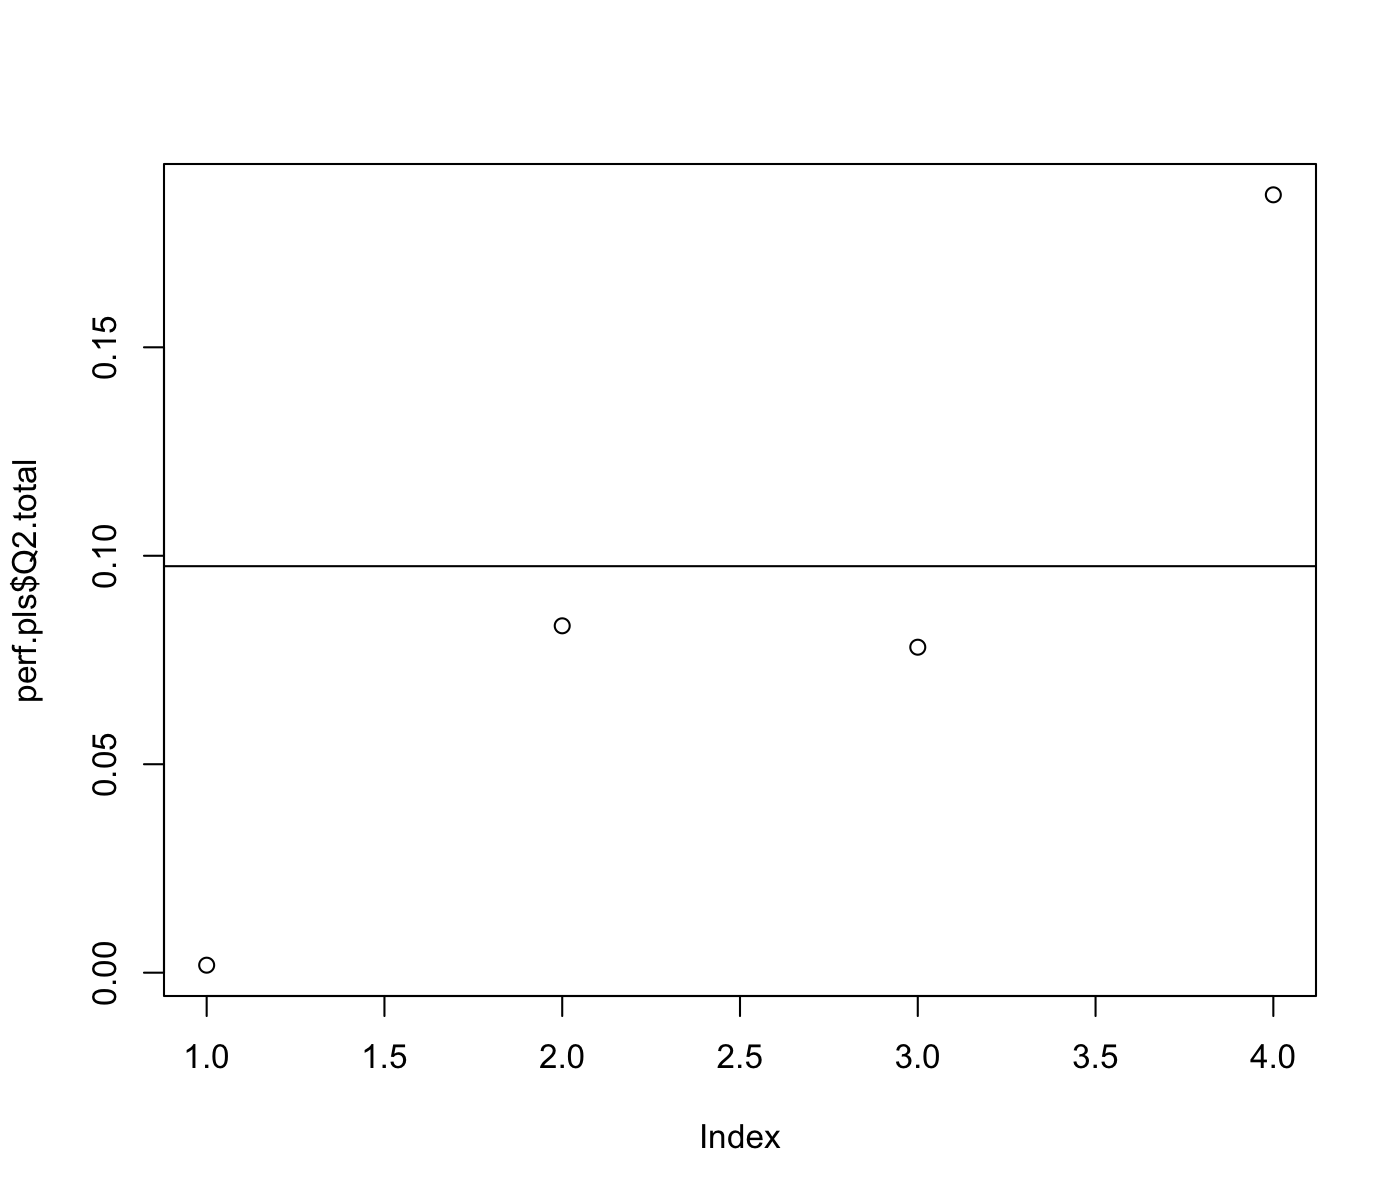
\includegraphics[width=0.5\linewidth]{Figures/unnamed-chunk-11-1} \end{center}

Interestingly from this plot, we can see that all selected variables on
component 1 are highly expressed in the BL (orange) class. Setting
\texttt{contrib\ =\ \textquotesingle{}min\textquotesingle{}} would
highlight that those variables are lowly expressed in the NB grey class,
which makes sense when we look at the sample plot.

Since 4 classes are being discriminated here, samples plots in 3d may
help interpretation:

\begin{Shaded}
\begin{Highlighting}[]
\KeywordTok{plotIndiv}\NormalTok{(MyResult.splsda2, }\DataTypeTok{style=}\StringTok{"3d"}\NormalTok{)}
\end{Highlighting}
\end{Shaded}

\subsection{Tuning parameters and numerical
outputs}\label{tuning:sPLSDA}

For this set of methods, three parameters need to be chosen:

1 - The number of components to retain \texttt{ncomp}. The rule of thumb
is usually \(K - 1\) where \(K\) is the number of classes, but it is
worth testing a few extra components.

2 - The number of variables \texttt{keepX} to select on each component
for sparse PLS-DA,

3 - The prediction distance to evaluate the classification and
prediction performance of PLS-DA.

For \textbf{item 1}, the \texttt{perf} evaluates the performance of
PLS-DA for a large number of components, using repeated k-fold
cross-validation. For example here we use 3-fold CV repeated 10 times
(note that we advise to use at least 50 repeats, and choose the number
of folds that are appropriate for the sample size of the data set):

\begin{Shaded}
\begin{Highlighting}[]
\NormalTok{MyResult.plsda2 <-}\StringTok{ }\KeywordTok{plsda}\NormalTok{(X,Y, }\DataTypeTok{ncomp=}\DecValTok{10}\NormalTok{)}
\KeywordTok{set.seed}\NormalTok{(}\DecValTok{30}\NormalTok{) }\CommentTok{# for reproducbility in this vignette, otherwise increase nrepeat}
\NormalTok{MyPerf.plsda <-}\StringTok{ }\KeywordTok{perf}\NormalTok{(MyResult.plsda2, }\DataTypeTok{validation =} \StringTok{"Mfold"}\NormalTok{, }\DataTypeTok{folds =} \DecValTok{3}\NormalTok{, }
                  \DataTypeTok{progressBar =} \OtherTok{FALSE}\NormalTok{, }\DataTypeTok{nrepeat =} \DecValTok{10}\NormalTok{) }\CommentTok{# we suggest nrepeat = 50}

\KeywordTok{plot}\NormalTok{(MyPerf.plsda, }\DataTypeTok{col =} \KeywordTok{color.mixo}\NormalTok{(}\DecValTok{5}\OperatorTok{:}\DecValTok{7}\NormalTok{), }\DataTypeTok{sd =} \OtherTok{TRUE}\NormalTok{, }\DataTypeTok{legend.position =} \StringTok{"horizontal"}\NormalTok{)}
\end{Highlighting}
\end{Shaded}

\begin{center}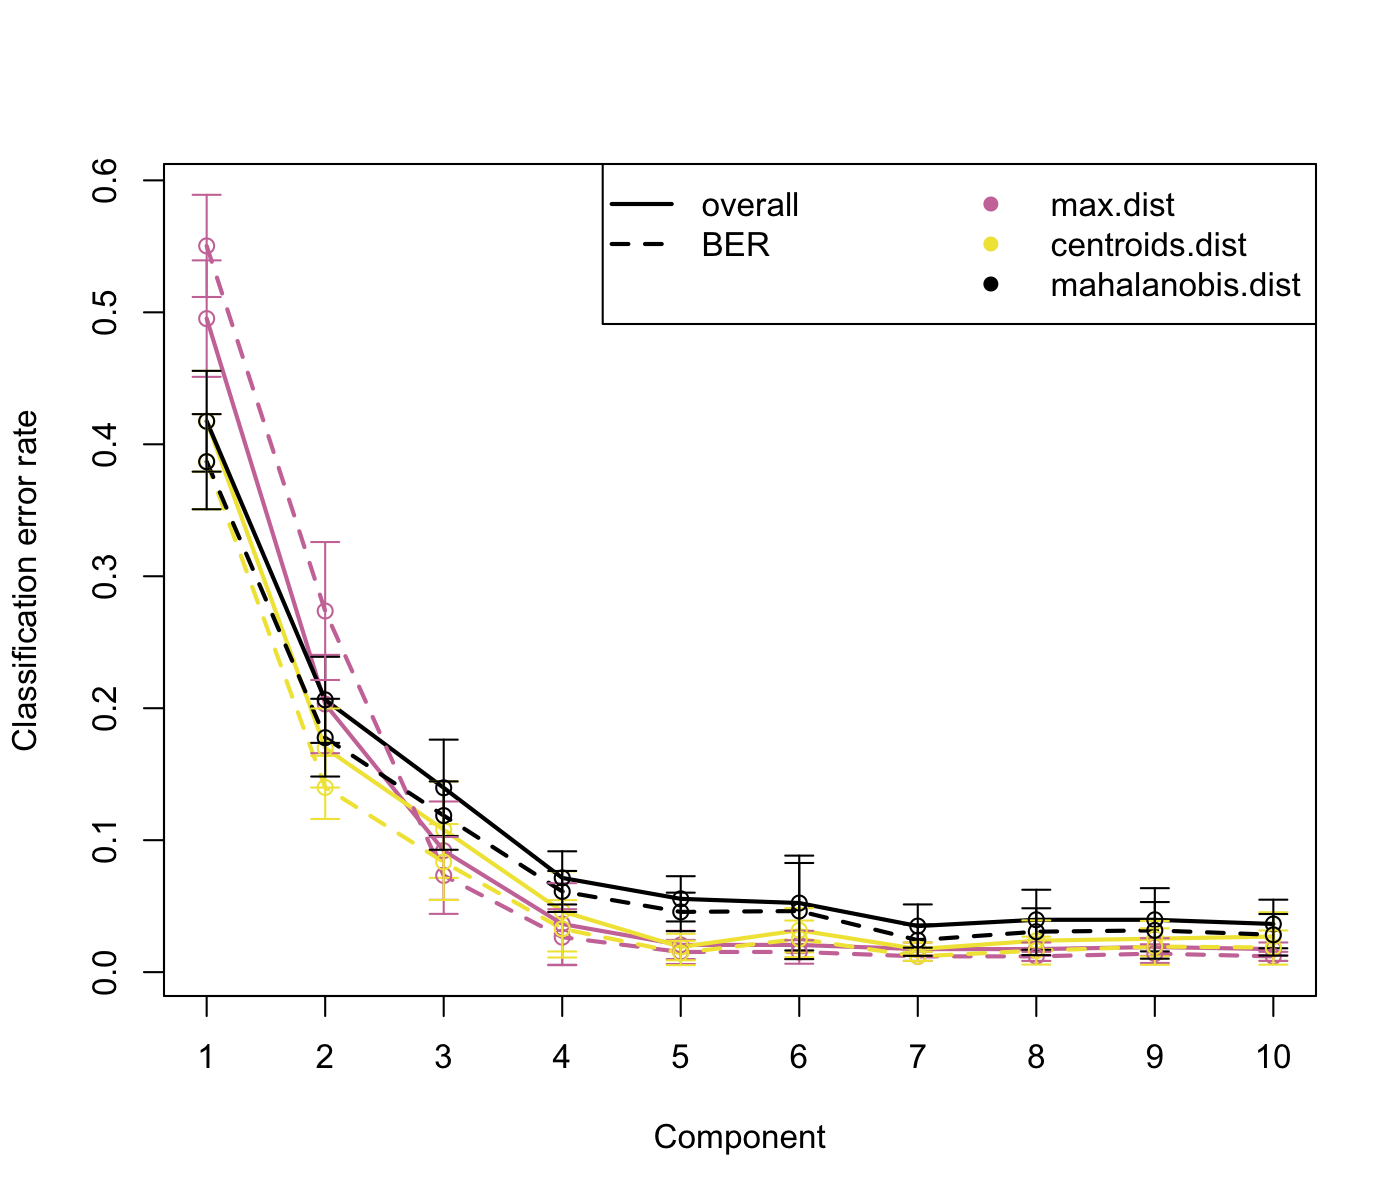
\includegraphics[width=0.5\linewidth]{Figures/unnamed-chunk-13-1} \end{center}

The plot outputs the classification error rate, or \emph{Balanced}
classification error rate when the number of samples per group is
unbalanced, the standard deviation according to three prediction
distances. Here we can see that for the BER and the maximum distance,
the best performance (i.e.~low error rate) seems to be achieved for
\texttt{ncomp\ =\ 3}.

In addition for \textbf{item 3} for PLS-DA, the numerical outputs listed
here can be reported as performance measures:

\begin{Shaded}
\begin{Highlighting}[]
\NormalTok{MyPerf.plsda}
\end{Highlighting}
\end{Shaded}

\begin{verbatim}
## 
## Call:
##  perf.plsda(object = MyResult.plsda2, validation = "Mfold", folds = 3, nrepeat = 10, progressBar = FALSE) 
## 
##  Main numerical outputs: 
##  -------------------- 
##  Error rate (overall or BER) for each component and for each distance: see object$error.rate 
##  Error rate per class, for each component and for each distance: see object$error.rate.class 
##  Prediction values for each component: see object$predict 
##  Classification of each sample, for each component and for each distance: see object$class 
##  AUC values: see object$auc if auc = TRUE 
## 
##  Visualisation Functions: 
##  -------------------- 
##  plot
\end{verbatim}

Regarding \textbf{item 2}, we now use \texttt{tune.splsda} to assess the
optimal number of variables to select on each component. We first set up
a grid of \texttt{keepX} values that will be assessed on each component,
one component at a time. Similar to above we run 3-fold CV repeated 10
times with a maximum distance prediction defined as above.

\begin{Shaded}
\begin{Highlighting}[]
\NormalTok{list.keepX <-}\StringTok{ }\KeywordTok{c}\NormalTok{(}\DecValTok{5}\OperatorTok{:}\DecValTok{10}\NormalTok{,  }\KeywordTok{seq}\NormalTok{(}\DecValTok{20}\NormalTok{, }\DecValTok{100}\NormalTok{, }\DecValTok{10}\NormalTok{))}
\NormalTok{list.keepX }\CommentTok{# to output the grid of values tested}
\end{Highlighting}
\end{Shaded}

\begin{verbatim}
##  [1]   5   6   7   8   9  10  20  30  40  50  60  70  80  90 100
\end{verbatim}

\begin{Shaded}
\begin{Highlighting}[]
\KeywordTok{set.seed}\NormalTok{(}\DecValTok{30}\NormalTok{) }\CommentTok{# for reproducbility in this vignette, otherwise increase nrepeat}
\NormalTok{tune.splsda.srbct <-}\StringTok{ }\KeywordTok{tune.splsda}\NormalTok{(X, Y, }\DataTypeTok{ncomp =} \DecValTok{3}\NormalTok{, }\CommentTok{# we suggest to push ncomp a bit more, e.g. 4}
                                 \DataTypeTok{validation =} \StringTok{'Mfold'}\NormalTok{,}
                                 \DataTypeTok{folds =} \DecValTok{3}\NormalTok{, }\DataTypeTok{dist =} \StringTok{'max.dist'}\NormalTok{, }\DataTypeTok{progressBar =} \OtherTok{FALSE}\NormalTok{,}
                                 \DataTypeTok{measure =} \StringTok{"BER"}\NormalTok{, }\DataTypeTok{test.keepX =}\NormalTok{ list.keepX,}
                                 \DataTypeTok{nrepeat =} \DecValTok{10}\NormalTok{)   }\CommentTok{# we suggest nrepeat = 50}
\end{Highlighting}
\end{Shaded}

We can then extract the classification error rate averaged across all
folds and repeats for each tested \texttt{keepX} value, the optimal
number of components (see \texttt{?tune.splsda} for more details), the
optimal number of variables to select per component which is summarised
in a plot where the diamond indicated the optimal \texttt{keepX} value:

\begin{Shaded}
\begin{Highlighting}[]
\NormalTok{error <-}\StringTok{ }\NormalTok{tune.splsda.srbct}\OperatorTok{$}\NormalTok{error.rate}
\NormalTok{ncomp <-}\StringTok{ }\NormalTok{tune.splsda.srbct}\OperatorTok{$}\NormalTok{choice.ncomp}\OperatorTok{$}\NormalTok{ncomp }\CommentTok{# optimal number of components based on t-tests on the error rate}
\NormalTok{ncomp}
\end{Highlighting}
\end{Shaded}

\begin{verbatim}
## [1] 3
\end{verbatim}

\begin{Shaded}
\begin{Highlighting}[]
\NormalTok{select.keepX <-}\StringTok{ }\NormalTok{tune.splsda.srbct}\OperatorTok{$}\NormalTok{choice.keepX[}\DecValTok{1}\OperatorTok{:}\NormalTok{ncomp]  }\CommentTok{# optimal number of variables to select}
\NormalTok{select.keepX}
\end{Highlighting}
\end{Shaded}

\begin{verbatim}
## comp1 comp2 comp3 
##    50    50    70
\end{verbatim}

\begin{Shaded}
\begin{Highlighting}[]
\KeywordTok{plot}\NormalTok{(tune.splsda.srbct, }\DataTypeTok{col =} \KeywordTok{color.jet}\NormalTok{(ncomp))}
\end{Highlighting}
\end{Shaded}

\begin{center}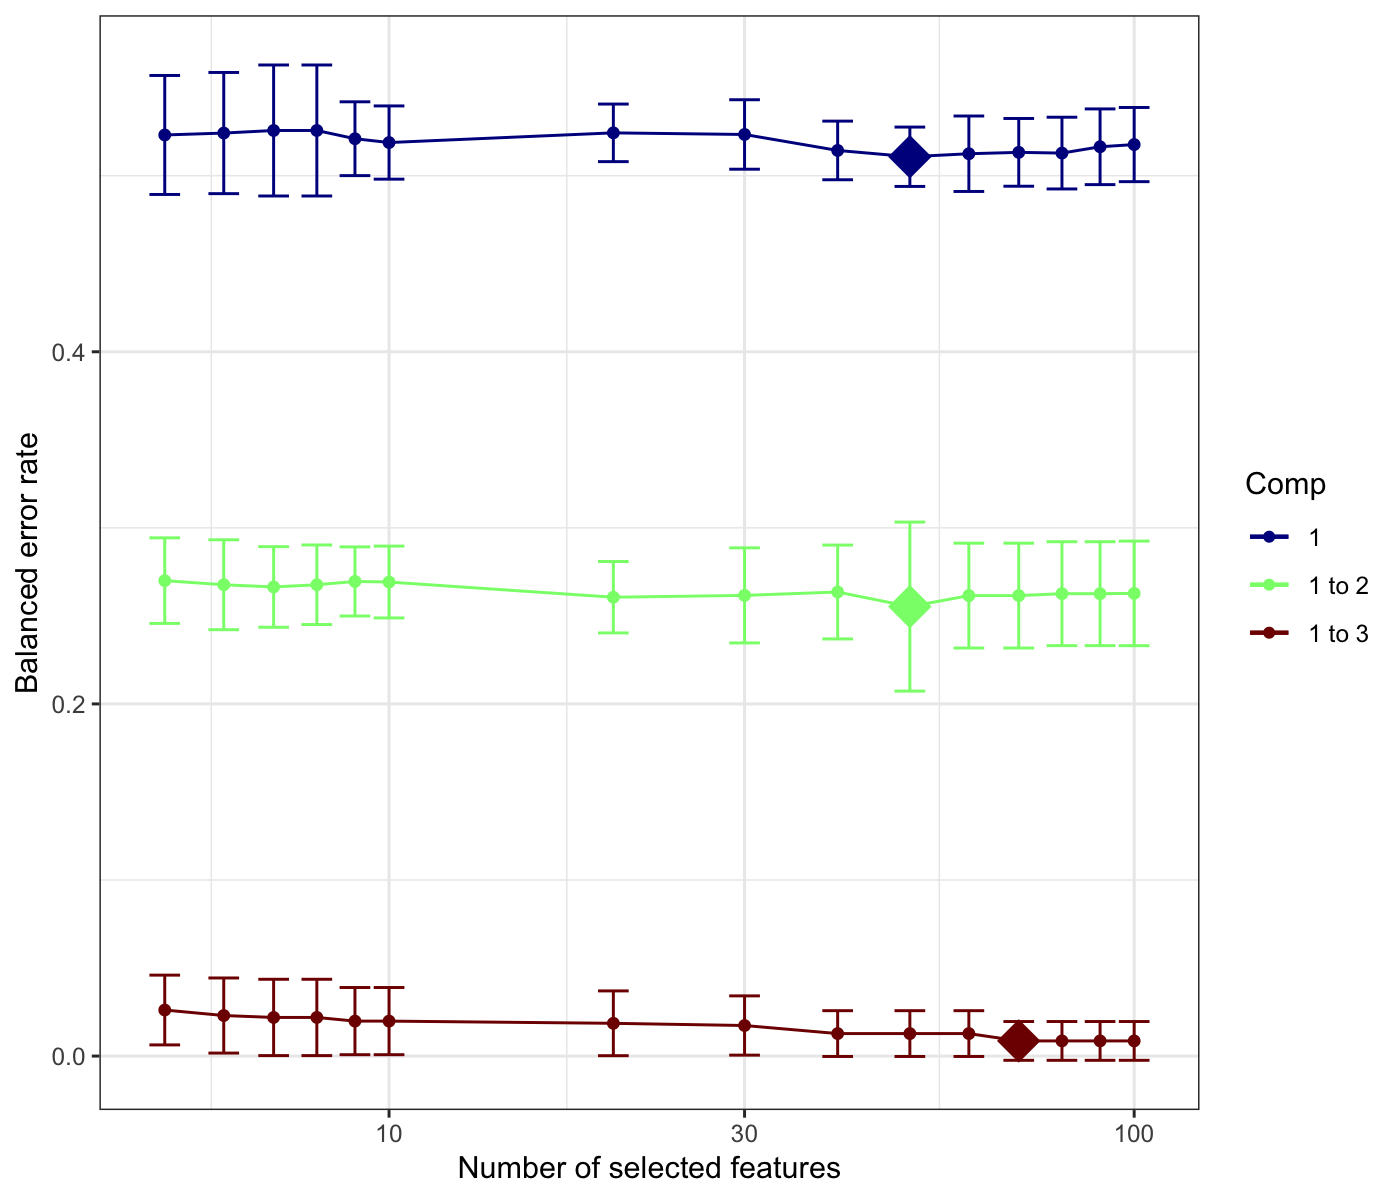
\includegraphics[width=0.5\linewidth]{Figures/unnamed-chunk-16-1} \end{center}

Based on those tuning results, we can run our final and tuned sPLS-DA
model:

\begin{Shaded}
\begin{Highlighting}[]
\NormalTok{MyResult.splsda.final <-}\StringTok{ }\KeywordTok{splsda}\NormalTok{(X, Y, }\DataTypeTok{ncomp =}\NormalTok{ ncomp, }\DataTypeTok{keepX =}\NormalTok{ select.keepX)}
\KeywordTok{plotIndiv}\NormalTok{(MyResult.splsda.final, }\DataTypeTok{ind.names =} \OtherTok{FALSE}\NormalTok{, }\DataTypeTok{legend=}\OtherTok{TRUE}\NormalTok{,}
          \DataTypeTok{ellipse =} \OtherTok{TRUE}\NormalTok{, }\DataTypeTok{title=}\StringTok{"SPLS-DA, Final result"}\NormalTok{)}
\end{Highlighting}
\end{Shaded}

Additionally we can run \texttt{perf} for the final performance of the
sPLS-DA model. Also note that \texttt{perf} will output
\texttt{features} that lists the frequency of selection of the variables
across the different folds and different repeats. This is a useful
output to assess the confidence of your final variable selection, see a
more \href{http://mixomics.org/case-studies/splsda-srbct/}{detailed
example here}.

\section{Additional resources}\label{additional-resources-1}

Additional examples are provided in \texttt{example(splsda)} and in our
case studies on our \href{http://www.mixomics.org}{website} in the
\textbf{Methods} and \textbf{Case studies} sections, and in particular
\href{http://mixomics.org/case-studies/splsda-srbct/}{here}. Also have a
look at \citep{Lec11}

\section{FAQ}\label{faq-1}

\begin{itemize}
\tightlist
\item
  Can I discriminate more than two groups of samples (multiclass
  classification)?

  \begin{itemize}
  \tightlist
  \item
    Yes, this is one of the advantage of PLS-DA, see this example above
  \end{itemize}
\item
  Can I have a hierarchy between two factors (e.g.~diet nested into
  genotype)?

  \begin{itemize}
  \tightlist
  \item
    Unfortunately no, sparse PLS-DA only allows to discriminate all
    groups at once (i.e.~4 x 2 groups when there are 4 diets and 2
    genotypes)
  \end{itemize}
\item
  Can I have missing values in my data?

  \begin{itemize}
  \tightlist
  \item
    Yes in the X data set, but you won't be able to do any prediction
    (i.e. \texttt{tune,\ perf,\ predict})
  \item
    No in the Y factor
  \end{itemize}
\end{itemize}

\chapter{Projection to Latent Structure (PLS)}\label{pls}

\begin{center}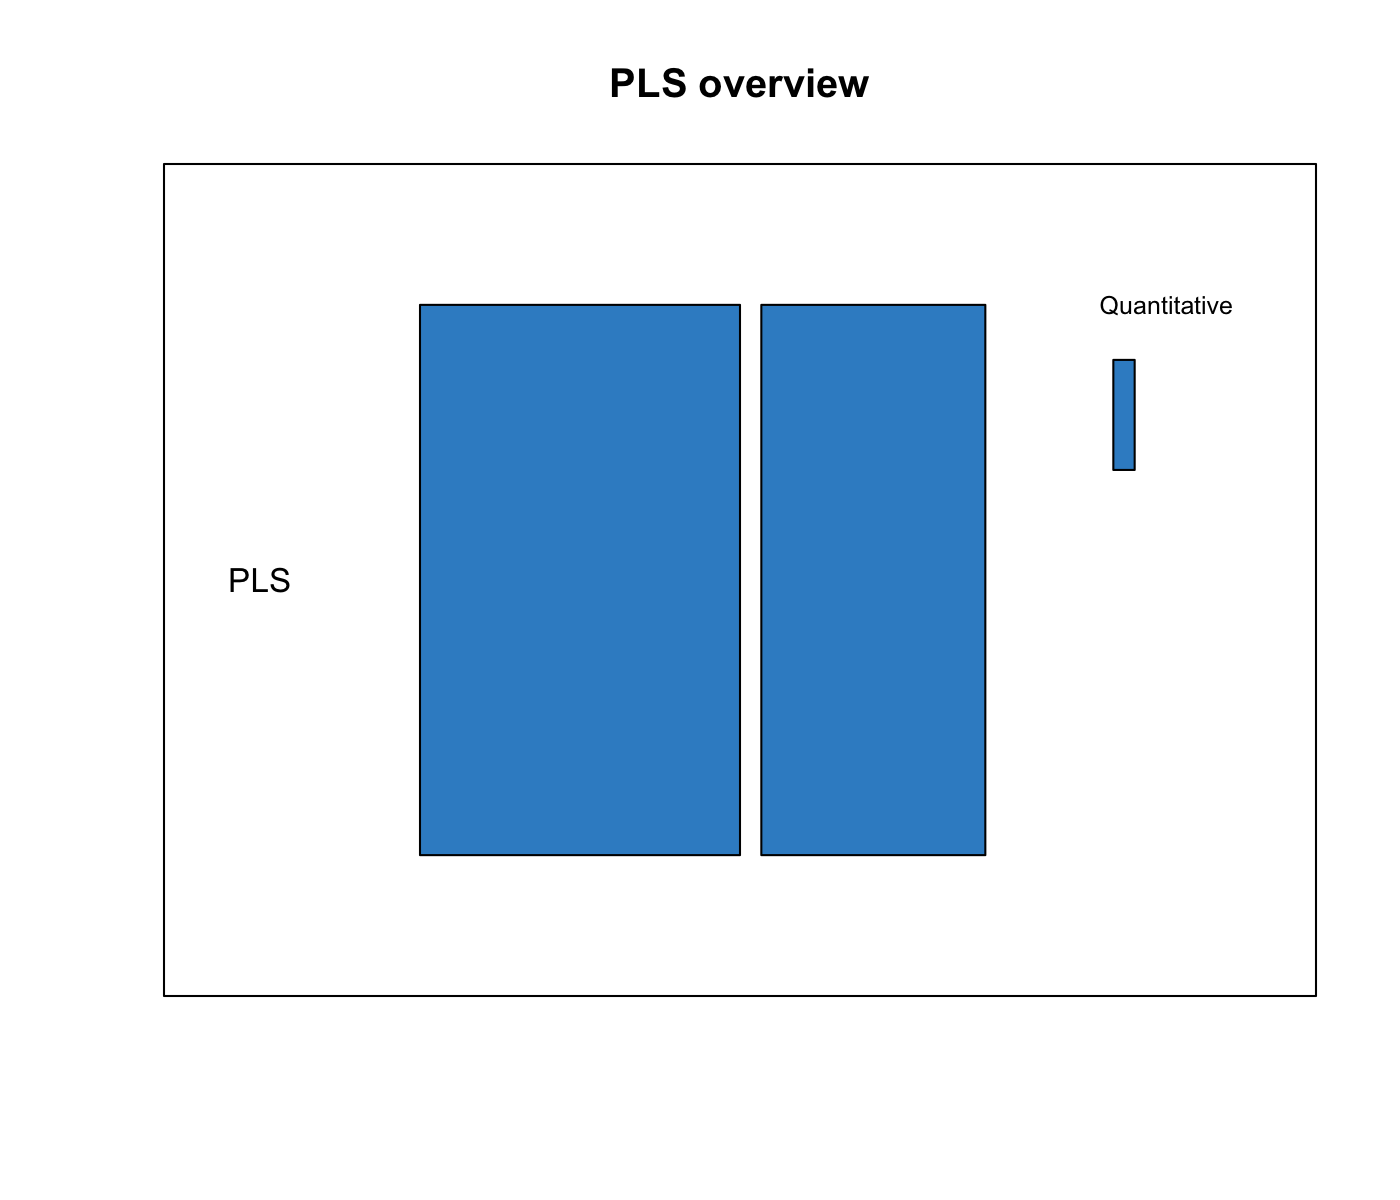
\includegraphics[width=0.5\linewidth]{Figures/overview-PLS-1} \end{center}

\section{Biological question}\label{biological-question-3}

{ \emph{I would like to integrate two data sets measured on the same
samples by extracting correlated information, or by highlighing
commonalities between data sets.} }

\section{\texorpdfstring{The \texttt{nutrimouse}
study}{The nutrimouse study}}\label{the-nutrimouse-study}

The \texttt{nutrimouse} study contains the expression levels of genes
potentially involved in nutritional problems and the concentrations of
hepatic fatty acids for forty mice. The data sets come from a
nutrigenomic study in the mouse from our collaborator \citep{Mar07}, in
which the effects of five regimens with contrasted fatty acid
compositions on liver lipids and hepatic gene expression in mice were
considered. Two sets of variables were measured on 40 mice:

\begin{itemize}
\item
  \texttt{gene}: the expression levels of 120 genes measured in liver
  cells, selected among (among about 30,000) as potentially relevant in
  the context of the nutrition study. These expressions come from a
  nylon microarray with radioactive labelling.
\item
  \texttt{lipid}: concentration (in percentage) of 21 hepatic fatty
  acids measured by gas chromatography.
\item
  \texttt{diet}: a 5-level factor. Oils used for experimental diets
  preparation were corn and colza oils (50/50) for a reference diet
  (REF), hydrogenated coconut oil for a saturated fatty acid diet (COC),
  sunflower oil for an Omega6 fatty acid-rich diet (SUN), linseed oil
  for an Omega3-rich diet (LIN) and corn/colza/enriched fish oils for
  the FISH diet (43/43/14).
\item
  \texttt{genotype} 2-levels factor indicating either wild-type (WT) and
  PPAR\(\alpha\) -/- (PPAR).
\end{itemize}

More details can be found in \texttt{?nutrimouse}.

To illustrate sparse PLS, we will integrate the gene expression levels
(\texttt{gene}) with the concentrations of hepatic fatty acids
(\texttt{lipid}).

\section{Principle of PLS}\label{principle-of-pls}

Partial Least Squares (PLS) regression \citep{Wol66, Wol01} is a
multivariate methodology which relates (\textit{integrates}) two data
matrices \texttt{X} (e.g.~transcriptomics) and \texttt{Y} (e.g.~lipids).
PLS goes beyond traditional multiple regression by modelling the
structure of both matrices. Unlike traditional multiple regression
models, it is not limited to uncorrelated variables. One of the many
advantages of PLS is that it can handle many noisy, collinear
(correlated) and missing variables and can also simultaneously model
several response variables in \texttt{Y}.

PLS is a multivariate projection-based method that can address different
types of integration problems. Its flexibility is the reason why it is
the backbone of most methods in \texttt{mixOmics}. PLS is
computationally very efficient when the number of variables
\(p + q >> n\) the number of samples. It performs successive local
regressions that avoid computational issues due to the inversion of
large singular covariance matrices. Unlike PCA which maximizes the
variance of components from a single data set, PLS maximizes the
covariance between components from two data sets. The mathematical
concepts of covariance and correlation are similar, but the covariance
is an unbounded measure and covariance has a unit measure (see
\ref{intro:background}). In PLS, linear combination of variables are
called \emph{latent variables} or \emph{latent components}. The weight
vectors used to calculate the linear combinations are called the
\emph{loading vectors}. Latent variables and loading vectors are thus
associated, and come in pairs from each of the two data sets being
integrated.

\section{Principle of sparse PLS}\label{principle-of-sparse-pls}

Even though PLS is highly efficient in a high dimensional context, the
interpretability of PLS needed to be improved. sPLS has been recently
developed by our team to perform simultaneous variable selection in both
data sets \texttt{X} and \texttt{Y} data sets, by including LASSO
\(\ell_1\) penalizations in PLS on each pair of loading vectors
\citep{Lec08}.

\section{Inputs and outputs}\label{inputs-and-outputs-1}

We consider the data input matrices: \texttt{X} is a \(n \times p\) data
matrix and \texttt{Y} a \(n \times q\) data matrix, where \(n\) the
number of samples (individuals), \(p\) and \(q\) are the number of
variables in each data set. PLS main outputs are:

\begin{itemize}
\item
  A \textbf{set of components}, also called latent variables associated
  to each data set. There are as many components as the chosen dimension
  of the PLS.
\item
  A \textbf{set of loading vectors}, which are coefficients assigned to
  each variable to define each component. Those coefficients indicate
  the importance of each variable in PLS. Importantly, each loading
  vector is associated to a particular component. Loading vectors are
  obtained so that the covariance between a linear combination of the
  variables from \texttt{X} (the X-component) and from \texttt{Y} (the
  \(Y\)-component) is maximised.
\item
  A \textbf{list of selected variables} from both \texttt{X} and
  \texttt{Y} and associated to each component if sPLS is applied.
\end{itemize}

\section{Set up the data}\label{set-up-the-data-1}

We first set up the data as \texttt{X} expression matrix and \texttt{Y}
as the lipid abundance matrix. We also check that the dimensions are
correct and match:

\begin{Shaded}
\begin{Highlighting}[]
\KeywordTok{library}\NormalTok{(mixOmics)}
\KeywordTok{data}\NormalTok{(nutrimouse)}
\NormalTok{X <-}\StringTok{ }\NormalTok{nutrimouse}\OperatorTok{$}\NormalTok{gene  }
\NormalTok{Y <-}\StringTok{ }\NormalTok{nutrimouse}\OperatorTok{$}\NormalTok{lipid}
\KeywordTok{dim}\NormalTok{(X); }\KeywordTok{dim}\NormalTok{(Y)}
\end{Highlighting}
\end{Shaded}

\begin{verbatim}
## [1]  40 120
\end{verbatim}

\begin{verbatim}
## [1] 40 21
\end{verbatim}

\section{Quick start}\label{quick-start-2}

We will mainly focus on sparse PLS for large biological data sets where
variable selection can help the interpretation of the results. See
\texttt{?pls} for a model with no variable selection. Here we
arbitrarily set the number of variables to select to 50 on each of the 2
components of PLS (see section \ref{tuning:PLS} for tuning these
values).

\begin{Shaded}
\begin{Highlighting}[]
\NormalTok{MyResult.spls <-}\StringTok{ }\KeywordTok{spls}\NormalTok{(X,Y, }\DataTypeTok{keepX =} \KeywordTok{c}\NormalTok{(}\DecValTok{25}\NormalTok{, }\DecValTok{25}\NormalTok{), }\DataTypeTok{keepY =} \KeywordTok{c}\NormalTok{(}\DecValTok{5}\NormalTok{,}\DecValTok{5}\NormalTok{))  }\CommentTok{# 1 Run the method}
\KeywordTok{plotIndiv}\NormalTok{(MyResult.spls)                                       }\CommentTok{# 2 Plot the samples}
\end{Highlighting}
\end{Shaded}

\begin{Shaded}
\begin{Highlighting}[]
\KeywordTok{plotVar}\NormalTok{(MyResult.spls)                                         }\CommentTok{# 3 Plot the  variables}
\end{Highlighting}
\end{Shaded}

If you were to run \texttt{spls} with this minimal code, you would be
using the following default values:

\begin{itemize}
\tightlist
\item
  \texttt{ncomp\ =\ 2}: the first two PLS components are calculated and
  are used for graphical outputs;
\item
  \texttt{scale\ =\ TRUE}: data are scaled (variance = 1, strongly
  advised here);
\item
  \texttt{mode\ =\ "regression"}: by default a PLS regression mode
  should be used (see \ref{PLS:details} for more details) .
\end{itemize}

Because PLS generates a pair of components, each associated to each data
set, the function \texttt{plotIndiv} produces 2 plots that represent the
same samples projected in either the space spanned by the X-components,
or the Y-components. A single plot can also be displayed, see section
\ref{pls:plotIndiv}.

\section{To go further}\label{pls-tgf}

\subsection{Customize sample plots}\label{pls:plotIndiv}

Some of the sample plot additional arguments were described in
\ref{splsda:plotIndiv}. In addition, you can choose the representation
space to be either the components from the \texttt{X}-data set, the
\texttt{Y}- data set, or an average between both components
\texttt{rep.space\ =\ \textquotesingle{}XY-variate\textquotesingle{}}.
See more examples in \texttt{examples(plotIndiv)} and on our
\href{http://mixomics.org/graphics/sample-plots/}{website}. Here are two
examples with colours indicating genotype or diet:

\begin{Shaded}
\begin{Highlighting}[]
\KeywordTok{plotIndiv}\NormalTok{(MyResult.spls, }\DataTypeTok{group =}\NormalTok{ nutrimouse}\OperatorTok{$}\NormalTok{genotype,}
          \DataTypeTok{rep.space =} \StringTok{"XY-variate"}\NormalTok{, }\DataTypeTok{legend =} \OtherTok{TRUE}\NormalTok{,}
          \DataTypeTok{legend.title =} \StringTok{'Genotype'}\NormalTok{,}
          \DataTypeTok{ind.names =}\NormalTok{ nutrimouse}\OperatorTok{$}\NormalTok{diet,}
          \DataTypeTok{title =} \StringTok{'Nutrimouse: sPLS'}\NormalTok{)}
\end{Highlighting}
\end{Shaded}

\begin{center}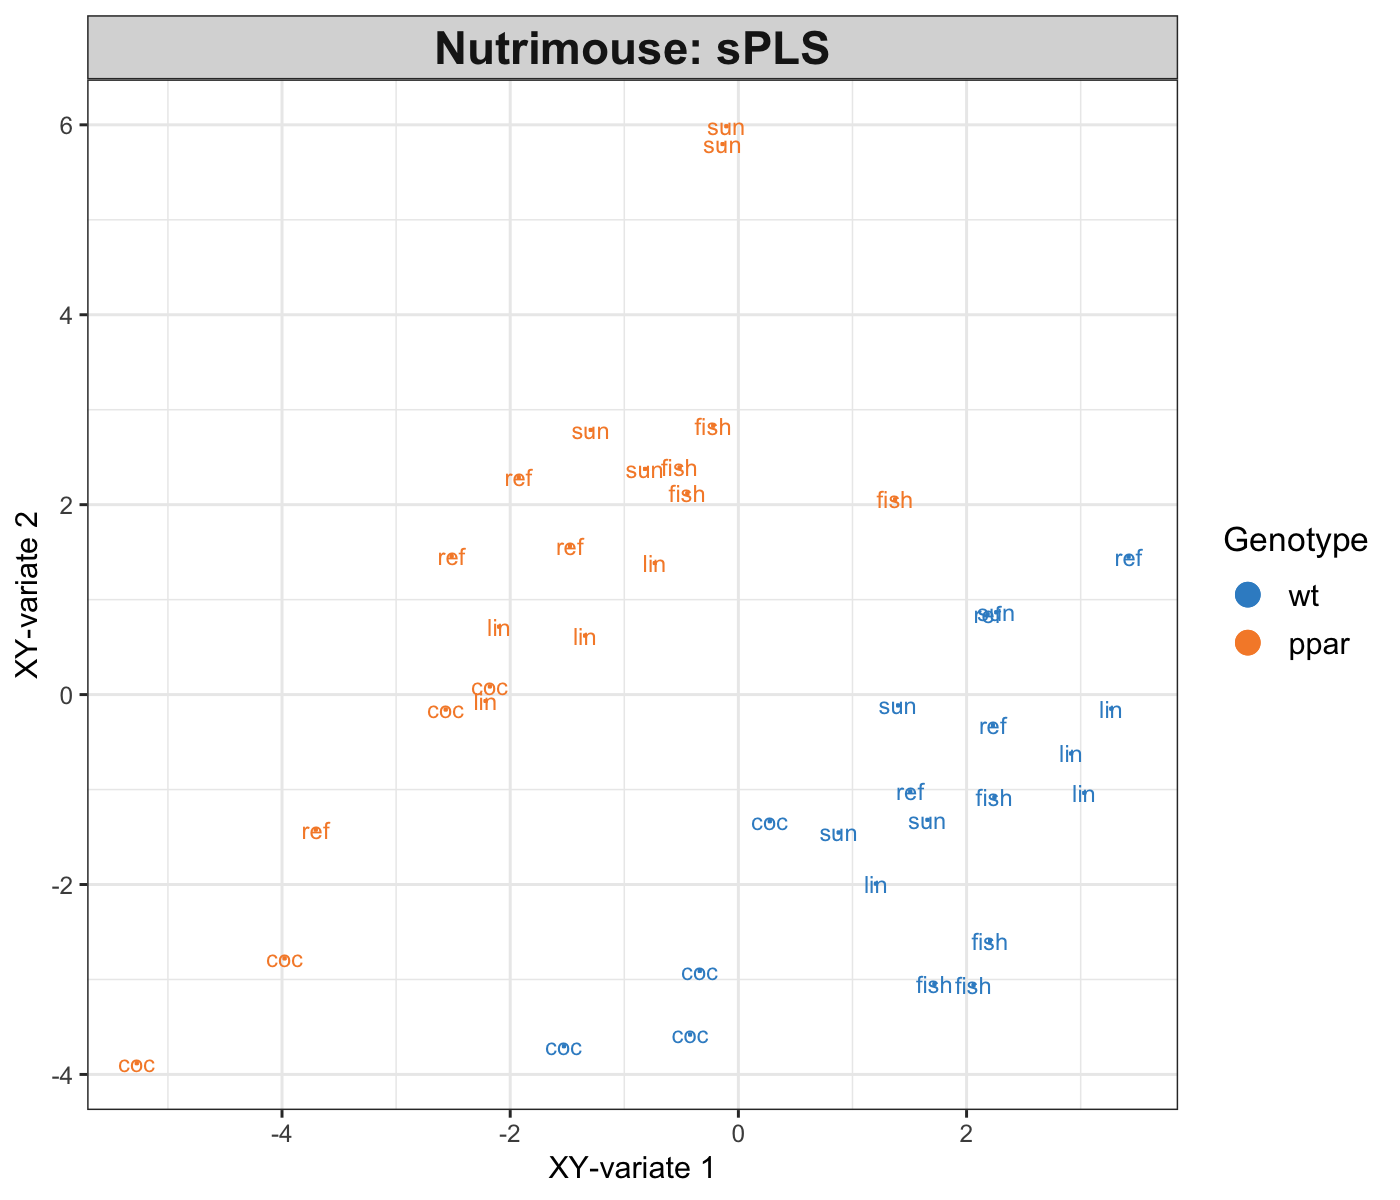
\includegraphics[width=0.5\linewidth]{Figures/unnamed-chunk-3-1} \end{center}

\begin{Shaded}
\begin{Highlighting}[]
\KeywordTok{plotIndiv}\NormalTok{(MyResult.spls, }\DataTypeTok{group=}\NormalTok{nutrimouse}\OperatorTok{$}\NormalTok{diet,}
          \DataTypeTok{pch =}\NormalTok{ nutrimouse}\OperatorTok{$}\NormalTok{genotype,}
          \DataTypeTok{rep.space =} \StringTok{"XY-variate"}\NormalTok{,  }\DataTypeTok{legend =} \OtherTok{TRUE}\NormalTok{,}
          \DataTypeTok{legend.title =} \StringTok{'Diet'}\NormalTok{, }\DataTypeTok{legend.title.pch =} \StringTok{'Genotype'}\NormalTok{,}
          \DataTypeTok{ind.names =} \OtherTok{FALSE}\NormalTok{, }
          \DataTypeTok{title =} \StringTok{'Nutrimouse: sPLS'}\NormalTok{)}
\end{Highlighting}
\end{Shaded}

\begin{center}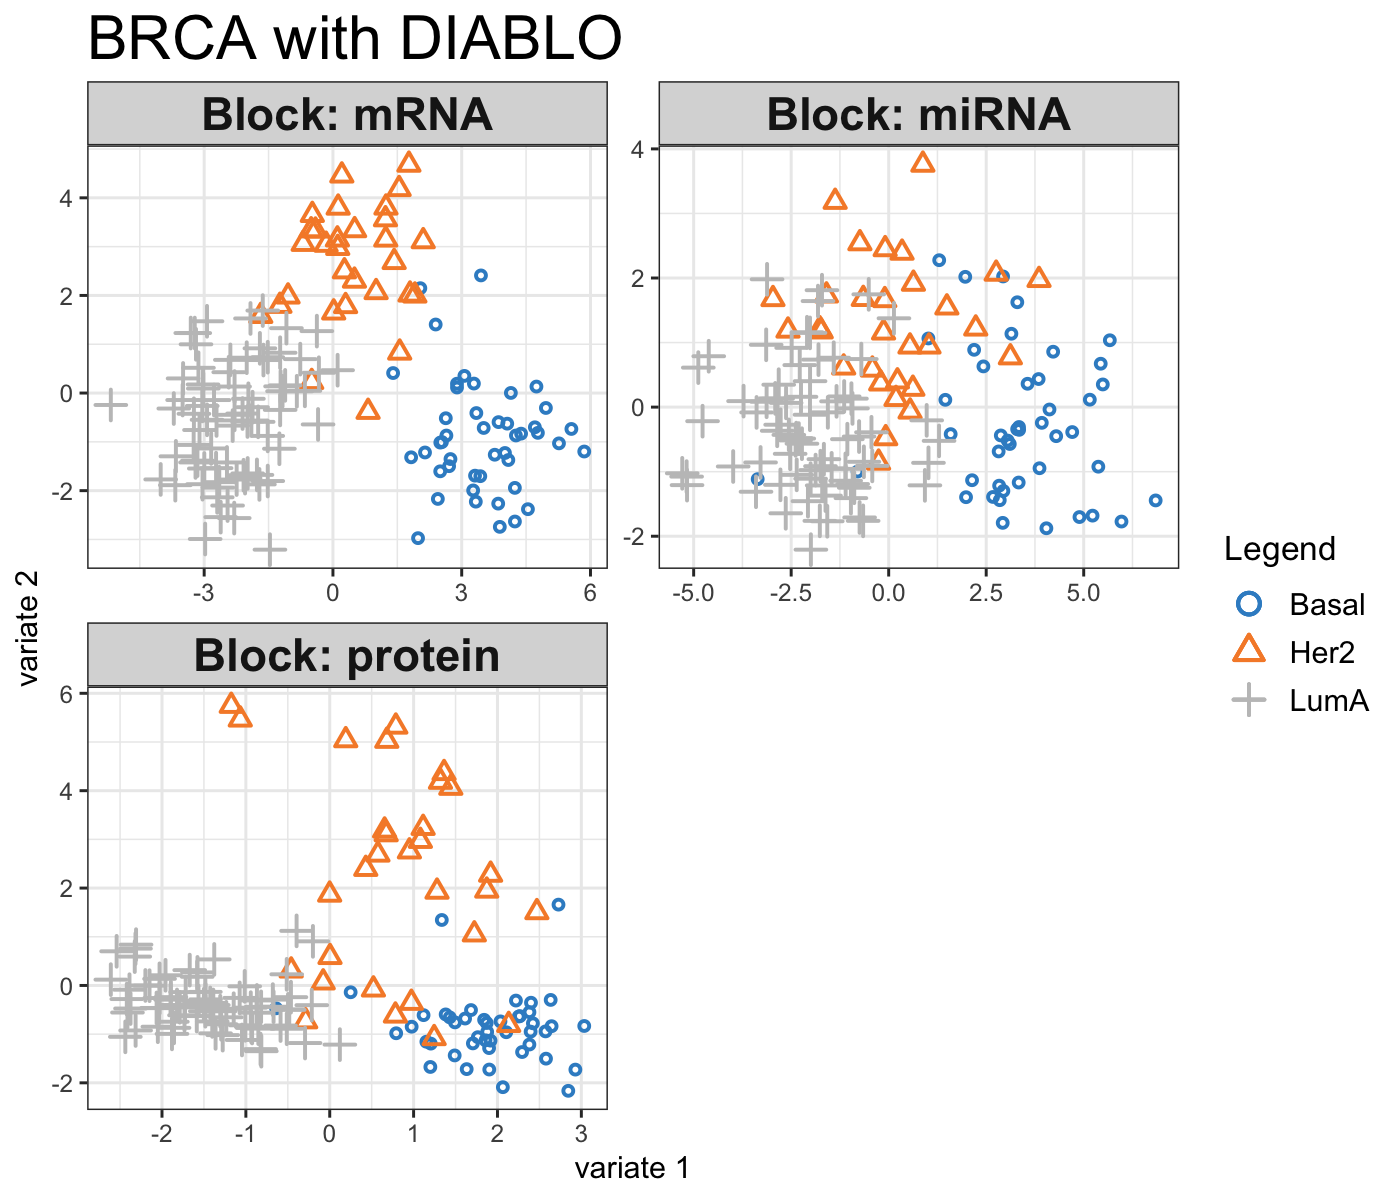
\includegraphics[width=0.5\linewidth]{Figures/unnamed-chunk-4-1} \end{center}

\subsection{Customize variable plots}\label{pls:plotVar}

See (\texttt{example(plotVar)}) for more examples. Here we change the
size of the labels. By default the colours are assigned to each type of
variable. The coordinates of the variables can also be saved as follows:

\begin{Shaded}
\begin{Highlighting}[]
\KeywordTok{plotVar}\NormalTok{(MyResult.spls, }\DataTypeTok{cex=}\KeywordTok{c}\NormalTok{(}\DecValTok{3}\NormalTok{,}\DecValTok{2}\NormalTok{), }\DataTypeTok{legend =} \OtherTok{TRUE}\NormalTok{)}
\end{Highlighting}
\end{Shaded}

\begin{center}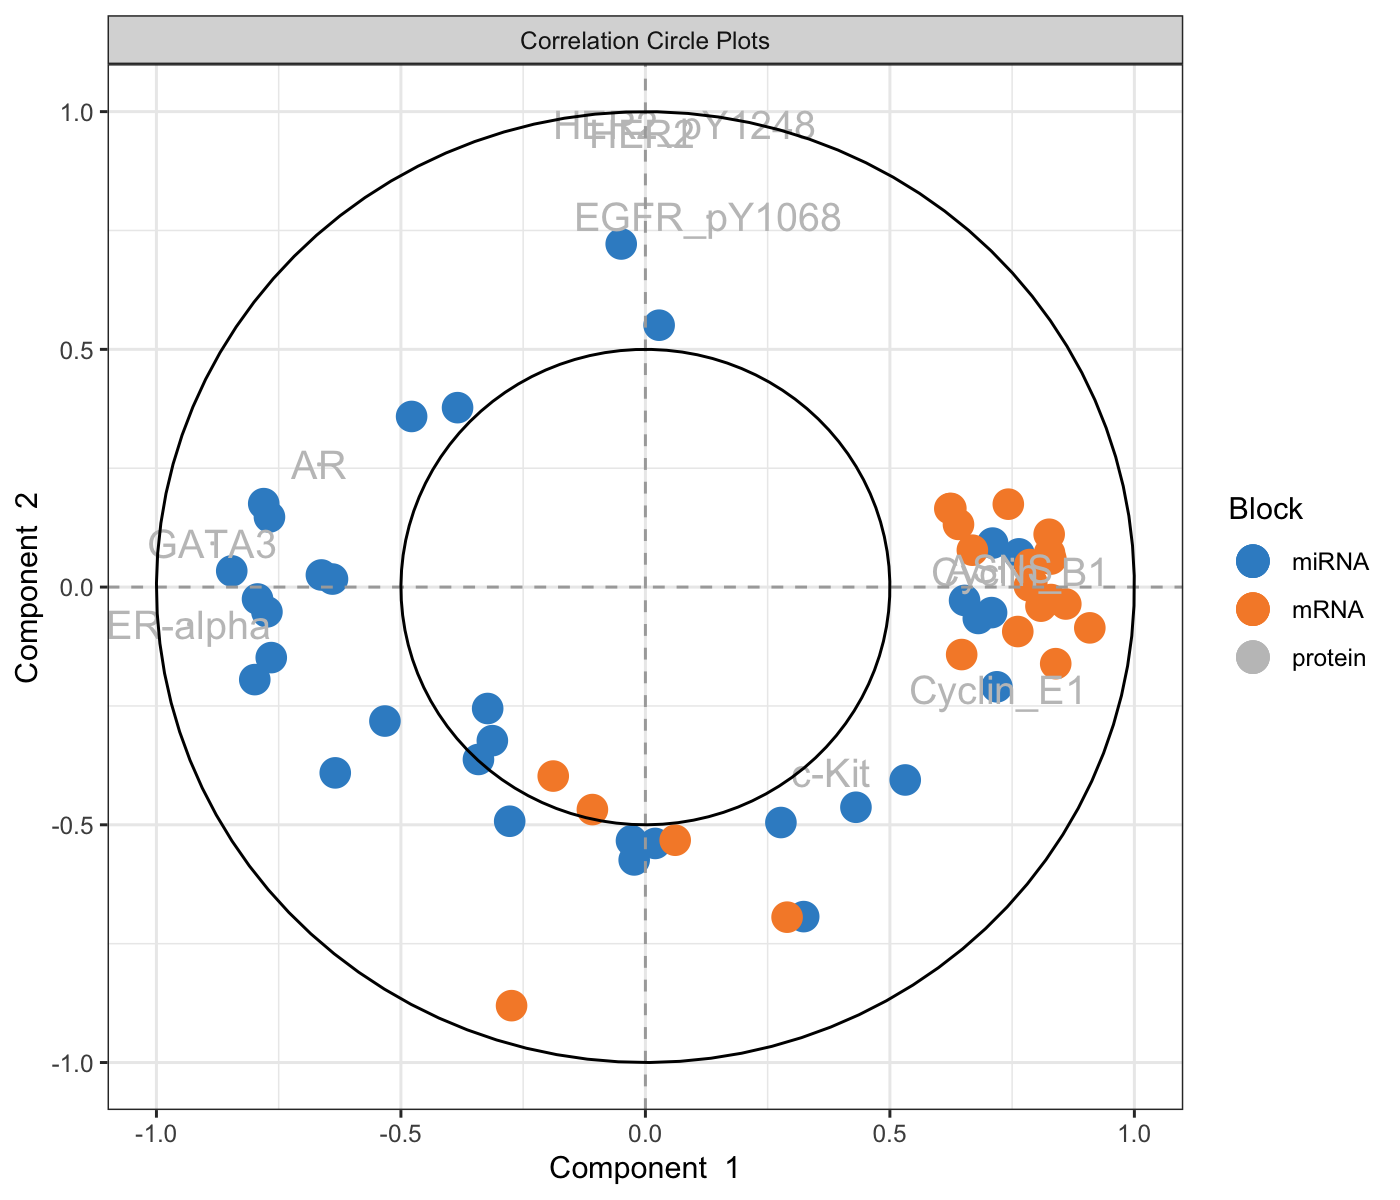
\includegraphics[width=0.5\linewidth]{Figures/unnamed-chunk-5-1} \end{center}

\begin{Shaded}
\begin{Highlighting}[]
\NormalTok{coordinates <-}\StringTok{ }\KeywordTok{plotVar}\NormalTok{(MyResult.spls, }\DataTypeTok{plot =} \OtherTok{FALSE}\NormalTok{)}
\end{Highlighting}
\end{Shaded}

\subsection{Other useful plots for data
integration}\label{other-useful-plots-for-data-integration}

We extended other types of plots, based on clustered image maps and
relevance networks to ease the interpretation of the relationships
between two types of variables. A similarity matrix is calculated from
the outputs of PLS and represented with those graphics, see
\citep{Gon12} for more details, and our
\href{http://mixomics.org/graphics/variable-plots/}{website}

\subsubsection{Clustered Image Maps}\label{clustered-image-maps}

A clustered image map can be produced using the \texttt{cim} function.
You may experience figures margin issues in RStudio. Best is to either
use \texttt{X11()} or save the plot as an external file. For example to
show the correlation structure between the X and Y variables selected on
component 1:

\begin{Shaded}
\begin{Highlighting}[]
\KeywordTok{X11}\NormalTok{()}
\KeywordTok{cim}\NormalTok{(MyResult.spls, }\DataTypeTok{comp =} \DecValTok{1}\NormalTok{)}
\KeywordTok{cim}\NormalTok{(MyResult.spls, }\DataTypeTok{comp =} \DecValTok{1}\NormalTok{, }\DataTypeTok{save =} \StringTok{'jpeg'}\NormalTok{, }\DataTypeTok{name.save =} \StringTok{'PLScim'}\NormalTok{)}
\end{Highlighting}
\end{Shaded}

\subsubsection{Relevance networks}\label{pls:network}

Using the same similarity matrix input in CIM, we can also represent
relevance bipartite networks. Those networks only represent edges
between on type of variable from \texttt{X} and the other type of
variable, from \texttt{Y}. Whilst we use sPLS to narrow down to a few
key correlated variables, our \texttt{keepX} and \texttt{keepY} values
might still be very high for this kind of output. A cut-off can be set
based on the correlation coefficient between the different types of
variables.

Other arguments such as \texttt{interactive\ =\ TRUE} enables a
scrollbar to change the cut-off value interactively, see other options
in \texttt{?network}. Additionally, the graph object can be saved to be
input into Cytoscape for an improved visualisation.

\begin{Shaded}
\begin{Highlighting}[]
\KeywordTok{X11}\NormalTok{()}
\KeywordTok{network}\NormalTok{(MyResult.spls, }\DataTypeTok{comp =} \DecValTok{1}\NormalTok{)}
\KeywordTok{network}\NormalTok{(MyResult.spls, }\DataTypeTok{comp =} \DecValTok{1}\NormalTok{, }\DataTypeTok{cutoff =} \FloatTok{0.6}\NormalTok{, }\DataTypeTok{save =} \StringTok{'jpeg'}\NormalTok{, }\DataTypeTok{name.save =} \StringTok{'PLSnetwork'}\NormalTok{)}
\CommentTok{# save as graph object for cytoscape}
\NormalTok{myNetwork <-}\StringTok{ }\KeywordTok{network}\NormalTok{(MyResult.spls, }\DataTypeTok{comp =} \DecValTok{1}\NormalTok{)}\OperatorTok{$}\NormalTok{gR}
\end{Highlighting}
\end{Shaded}

\subsubsection{Arrow plots}\label{arrow-plots}

Instead of projecting the samples into the combined XY representation
space, as shown in \ref{pls:plotIndiv}, we can overlap the X- and Y-
representation plots. One arrow joins the same sample from the X- space
to the Y- space. Short arrows indicate a good agreement found by the PLS
between both data sets.

\begin{Shaded}
\begin{Highlighting}[]
\KeywordTok{plotArrow}\NormalTok{(MyResult.spls,}\DataTypeTok{group=}\NormalTok{nutrimouse}\OperatorTok{$}\NormalTok{diet, }\DataTypeTok{legend =} \OtherTok{TRUE}\NormalTok{,}
          \DataTypeTok{X.label =} \StringTok{'PLS comp 1'}\NormalTok{, }\DataTypeTok{Y.label =} \StringTok{'PLS comp 2'}\NormalTok{)}
\end{Highlighting}
\end{Shaded}

\begin{center}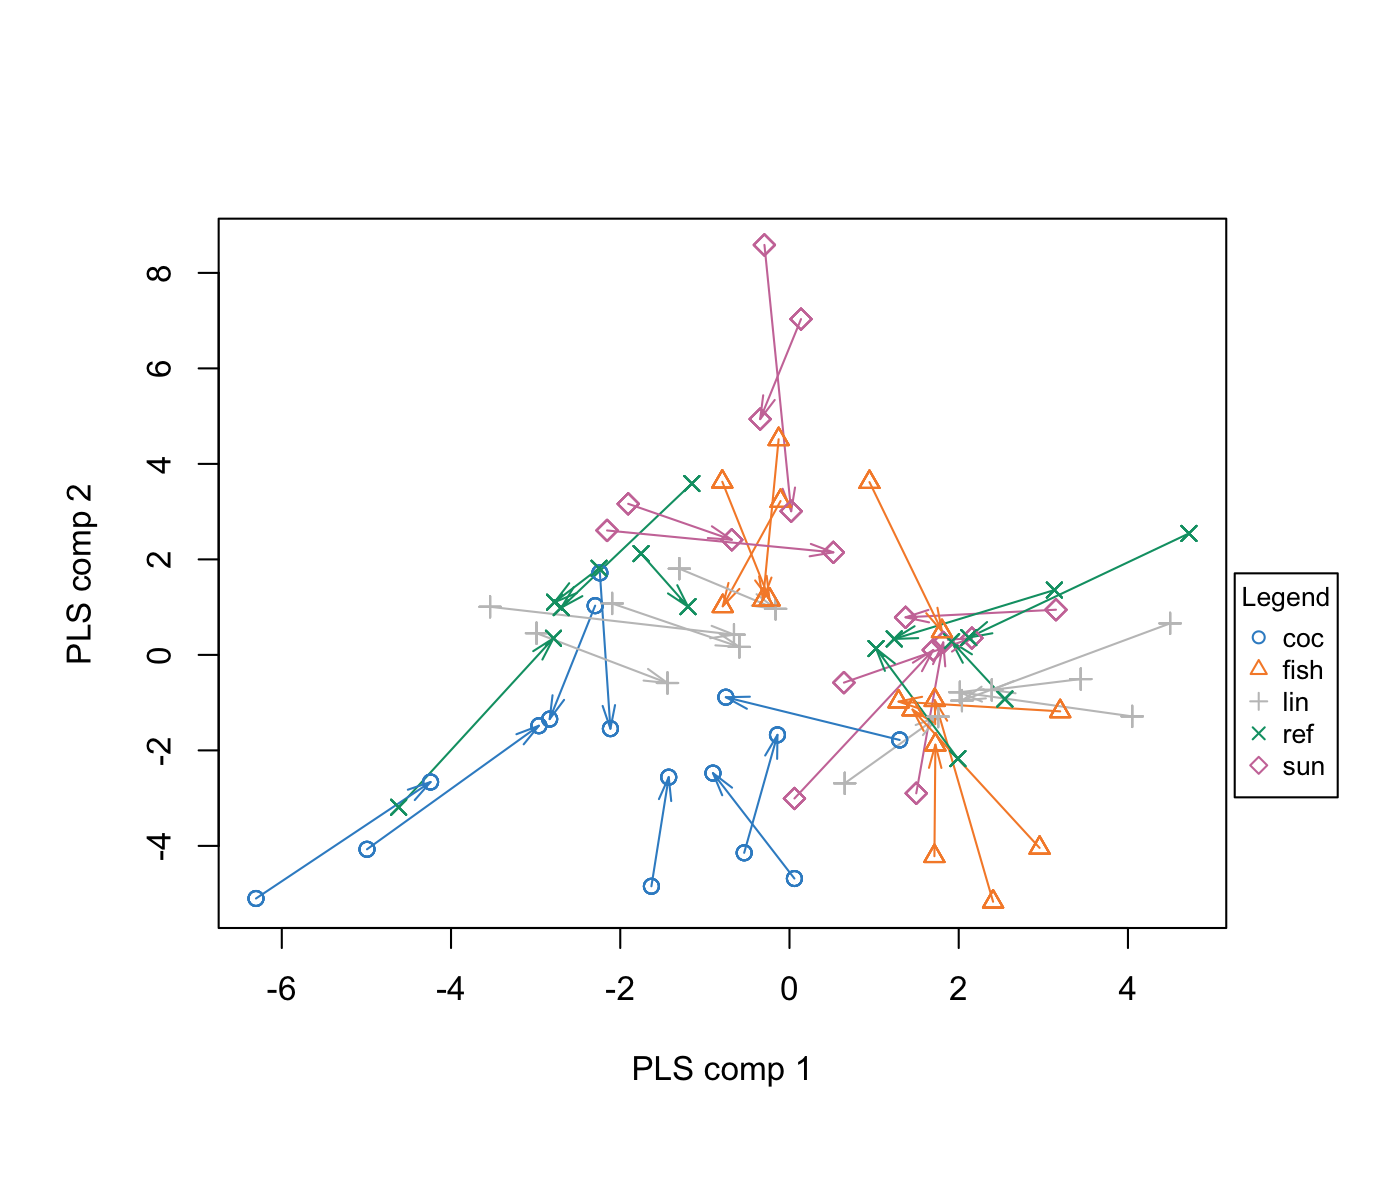
\includegraphics[width=0.5\linewidth]{Figures/unnamed-chunk-8-1} \end{center}

\subsection{Variable selection
outputs}\label{variable-selection-outputs-1}

The selected variables can be extracted using the \texttt{selectVar}
function for further analysis.

\begin{Shaded}
\begin{Highlighting}[]
\NormalTok{MySelectedVariables <-}\StringTok{ }\KeywordTok{selectVar}\NormalTok{(MyResult.spls, }\DataTypeTok{comp =} \DecValTok{1}\NormalTok{)}
\NormalTok{MySelectedVariables}\OperatorTok{$}\NormalTok{X}\OperatorTok{$}\NormalTok{name }\CommentTok{# Selected genes on component 1}
\end{Highlighting}
\end{Shaded}

\begin{verbatim}
##  [1] "SR.BI"   "SPI1.1"  "PMDCI"   "CYP3A11" "Ntcp"    "GSTpi2"  "FAT"    
##  [8] "apoC3"   "UCP2"    "CAR1"    "Waf1"    "ACOTH"   "eif2g"   "PDK4"   
## [15] "CYP4A10" "VDR"     "SIAT4c"  "RXRg1"   "RXRa"    "CBS"     "SHP1"   
## [22] "MCAD"    "MS"      "CYP4A14" "ALDH3"
\end{verbatim}

\begin{Shaded}
\begin{Highlighting}[]
\NormalTok{MySelectedVariables}\OperatorTok{$}\NormalTok{Y}\OperatorTok{$}\NormalTok{name }\CommentTok{# Selected lipids on component 1}
\end{Highlighting}
\end{Shaded}

\begin{verbatim}
## [1] "C18.0"    "C16.1n.9" "C18.1n.9" "C20.3n.6" "C22.6n.3"
\end{verbatim}

The loading plots help visualise the coefficients assigned to each
selected variable on each component:

\begin{Shaded}
\begin{Highlighting}[]
\KeywordTok{plotLoadings}\NormalTok{(MyResult.spls, }\DataTypeTok{comp =} \DecValTok{1}\NormalTok{, }\DataTypeTok{size.name =} \KeywordTok{rel}\NormalTok{(}\FloatTok{0.5}\NormalTok{))}
\end{Highlighting}
\end{Shaded}

\begin{center}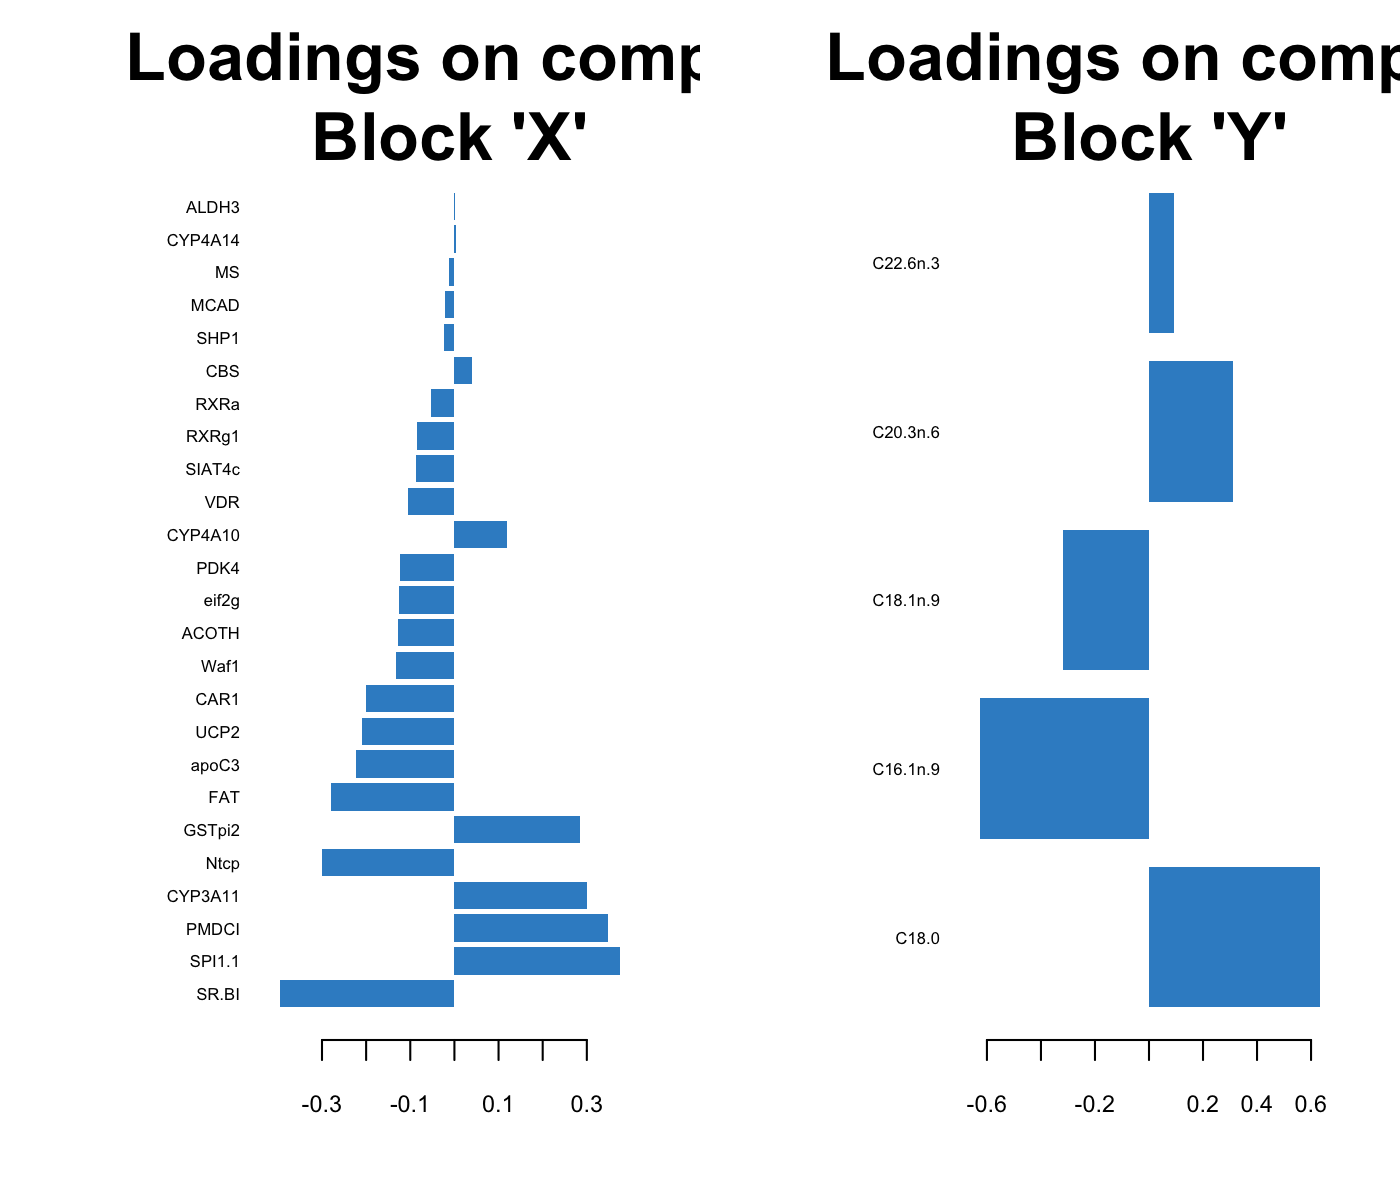
\includegraphics[width=0.5\linewidth]{Figures/unnamed-chunk-10-1} \end{center}

\subsection{Tuning parameters and numerical outputs}\label{tuning:PLS}

For PLS and sPLS, two types of parameters need to be chosen:

1 - The number of components to retain \texttt{ncomp}, 2 - The number of
variables to select on each component and on each data set
\texttt{keepX} and \texttt{keepY} for sparse PLS.

For \textbf{item 1} we use the \texttt{perf} function and repeated
k-fold cross-validation to calculate the Q\(^2\) criterion used in the
SIMCA-P software \citep{Ume96}. The rule of thumbs is that a PLS
component should be included in the model if its value is
\(\leq 0.0975\). Here we use 3-fold CV repeated 10 times (note that we
advise to use at least 50 repeats, and choose the number of folds that
are appropriate for the sample size of the data set).

We run a PLS model with a sufficient number of components first, then
run \texttt{perf} on the object.

\begin{Shaded}
\begin{Highlighting}[]
\NormalTok{MyResult.pls <-}\StringTok{ }\KeywordTok{pls}\NormalTok{(X,Y, }\DataTypeTok{ncomp =} \DecValTok{4}\NormalTok{)  }
\KeywordTok{set.seed}\NormalTok{(}\DecValTok{30}\NormalTok{) }\CommentTok{# for reproducbility in this vignette, otherwise increase nrepeat}
\NormalTok{perf.pls <-}\StringTok{ }\KeywordTok{perf}\NormalTok{(MyResult.pls, }\DataTypeTok{validation =} \StringTok{"Mfold"}\NormalTok{, }\DataTypeTok{folds =} \DecValTok{5}\NormalTok{,}
                  \DataTypeTok{progressBar =} \OtherTok{FALSE}\NormalTok{, }\DataTypeTok{nrepeat =} \DecValTok{10}\NormalTok{)}
\KeywordTok{plot}\NormalTok{(perf.pls}\OperatorTok{$}\NormalTok{Q2.total)}
\KeywordTok{abline}\NormalTok{(}\DataTypeTok{h =} \FloatTok{0.0975}\NormalTok{)}
\end{Highlighting}
\end{Shaded}

\begin{center}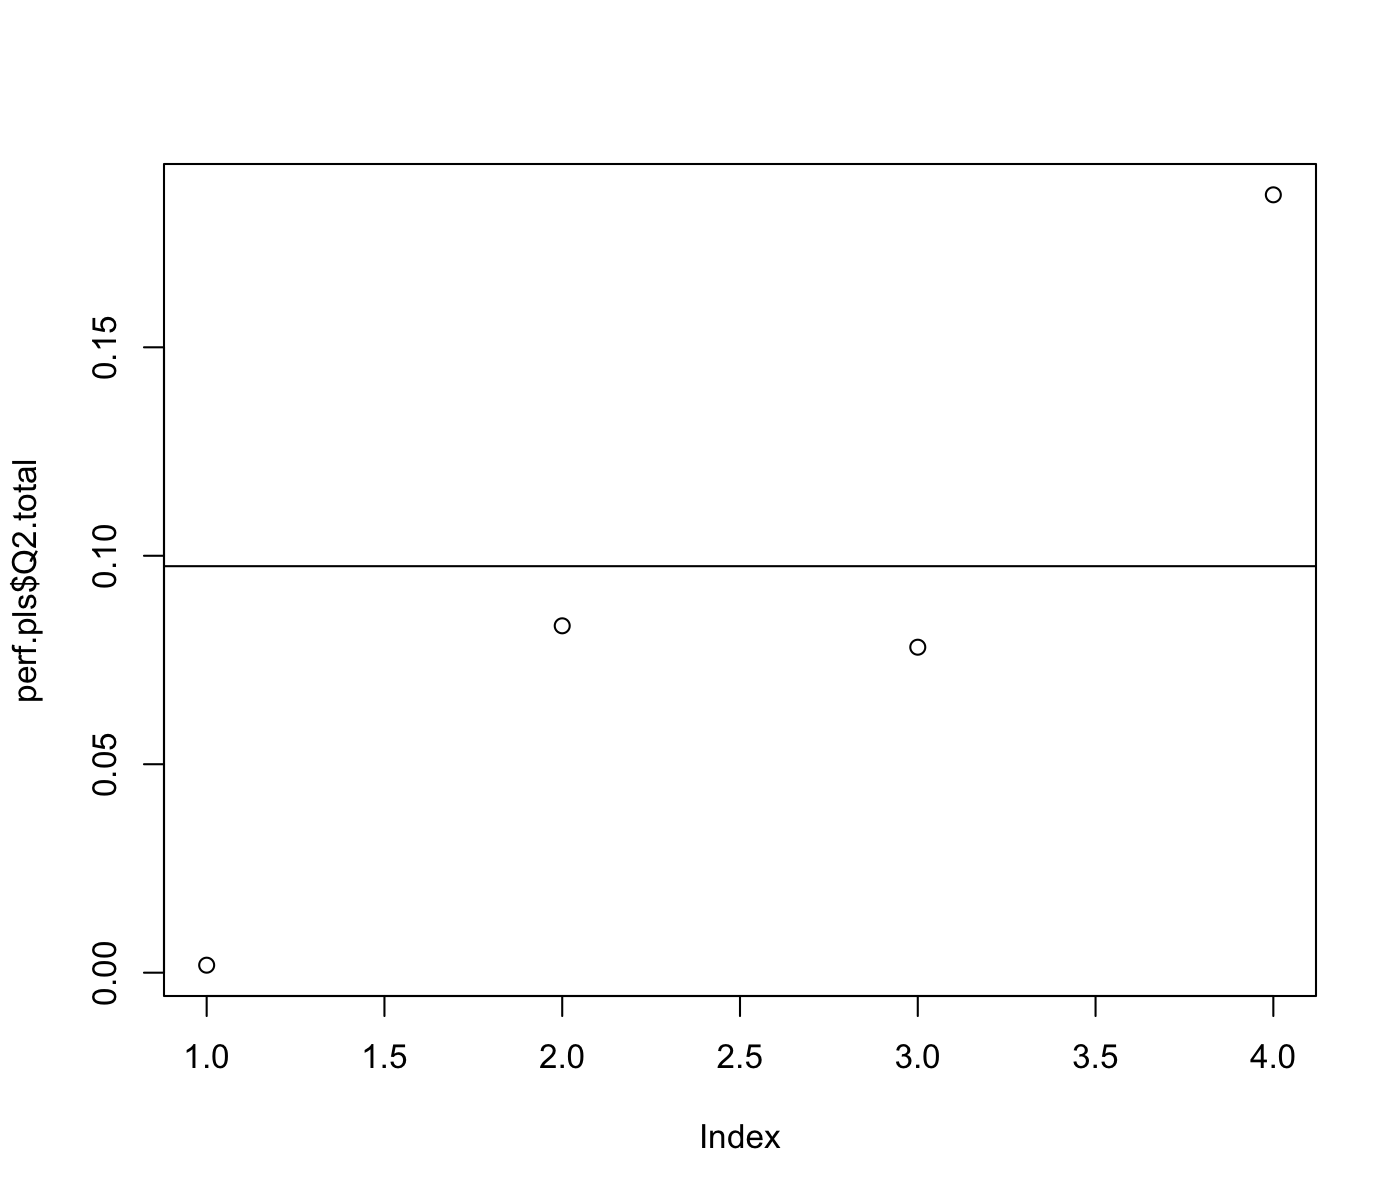
\includegraphics[width=0.5\linewidth]{Figures/unnamed-chunk-11-1} \end{center}

This example seems to indicate that up to 3 components could be enough.
In a small \(p+q\) setting we generally observe a Q\(^2\) that
decreases, but that is not the case here as \(n << p+q\).

\textbf{Item 2} can be quite difficult to tune. Here is a minimal
example where we only tune \texttt{keepX} based on the Mean Absolute
Value. Other measures proposed are Mean Square Error, Bias and R2 (see
\texttt{?tune.spls}):

\begin{Shaded}
\begin{Highlighting}[]
\NormalTok{list.keepX <-}\StringTok{ }\KeywordTok{c}\NormalTok{(}\DecValTok{2}\OperatorTok{:}\DecValTok{10}\NormalTok{, }\DecValTok{15}\NormalTok{, }\DecValTok{20}\NormalTok{)}
\CommentTok{# tuning based on MAE}
\KeywordTok{set.seed}\NormalTok{(}\DecValTok{30}\NormalTok{) }\CommentTok{# for reproducbility in this vignette, otherwise increase nrepeat}
\NormalTok{tune.spls.MAE <-}\StringTok{ }\KeywordTok{tune.spls}\NormalTok{(X, Y, }\DataTypeTok{ncomp =} \DecValTok{3}\NormalTok{,}
                           \DataTypeTok{test.keepX =}\NormalTok{ list.keepX,}
                           \DataTypeTok{validation =} \StringTok{"Mfold"}\NormalTok{, }\DataTypeTok{folds =} \DecValTok{5}\NormalTok{,}
                           \DataTypeTok{nrepeat =} \DecValTok{10}\NormalTok{, }\DataTypeTok{progressBar =} \OtherTok{FALSE}\NormalTok{,}
                           \DataTypeTok{measure =} \StringTok{'MAE'}\NormalTok{)}
\KeywordTok{plot}\NormalTok{(tune.spls.MAE, }\DataTypeTok{legend.position =} \StringTok{'topright'}\NormalTok{)}
\end{Highlighting}
\end{Shaded}

\begin{center}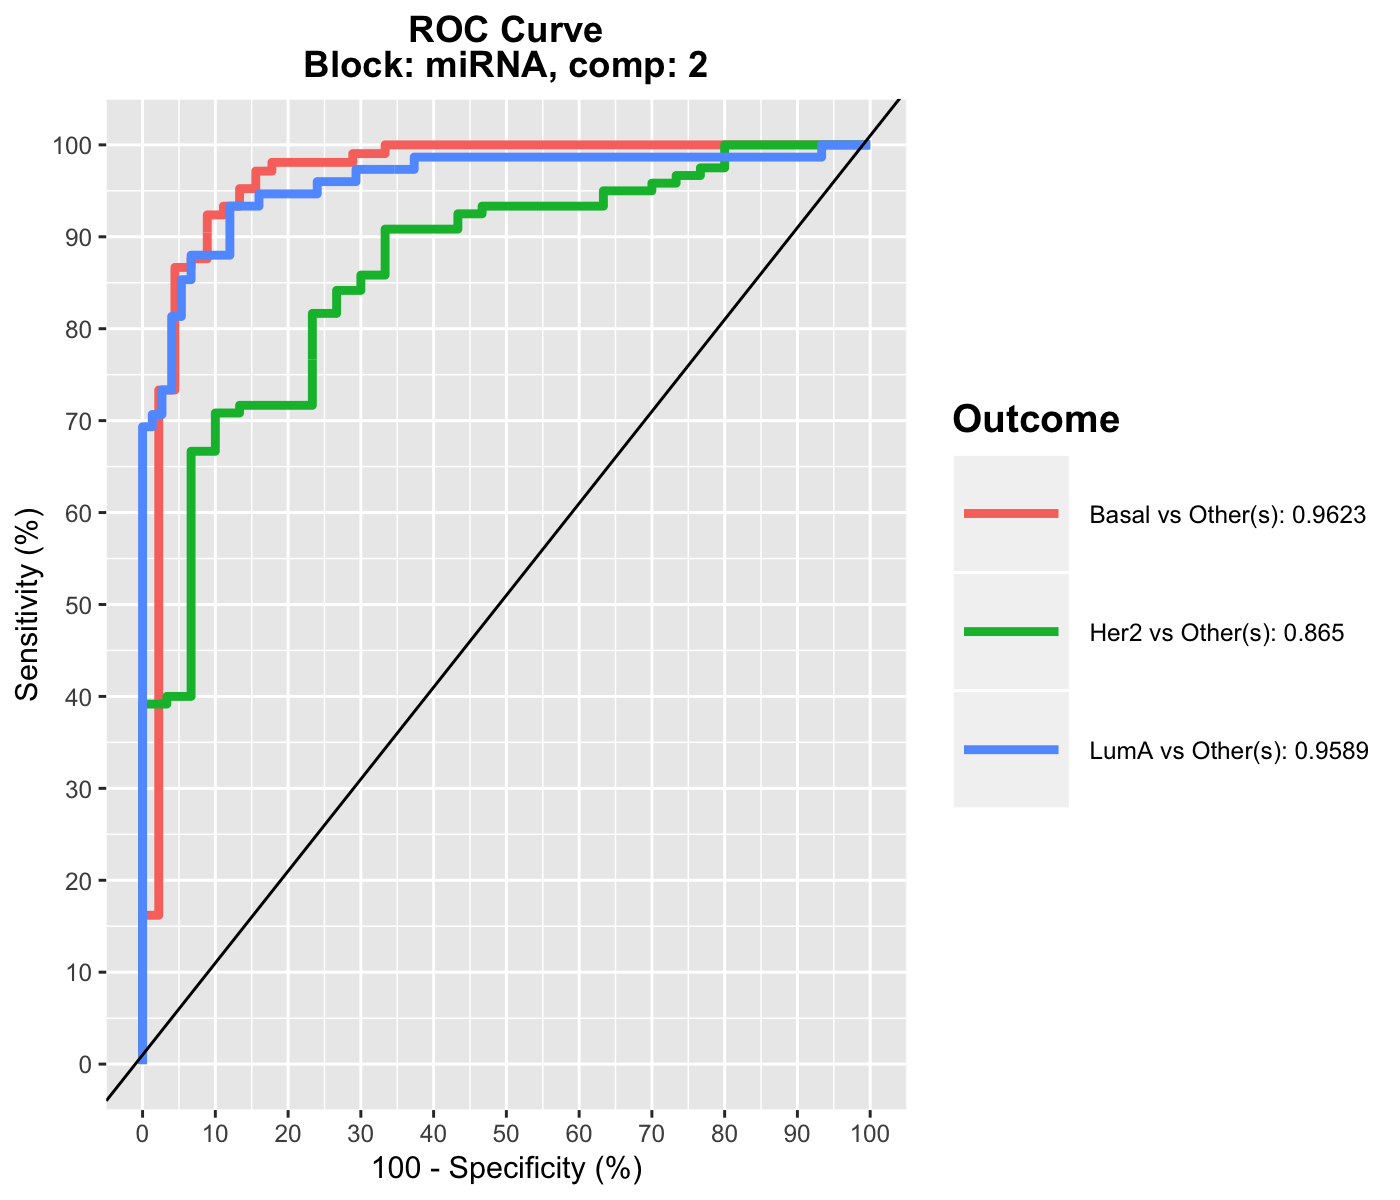
\includegraphics[width=0.5\linewidth]{Figures/unnamed-chunk-12-1} \end{center}

Based on the lowest MAE obtained on each component, the optimal number
of variables to select in the \texttt{X} data set, including all
variables in the \texttt{Y} data set would be:

\begin{Shaded}
\begin{Highlighting}[]
\NormalTok{tune.spls.MAE}\OperatorTok{$}\NormalTok{choice.keepX}
\end{Highlighting}
\end{Shaded}

\begin{verbatim}
## comp1 comp2 comp3 
##    15     2    20
\end{verbatim}

Tuning \texttt{keepX} and \texttt{keepY} conjointly is still work in
progress. What we advise in the meantime is either to adopt an arbitrary
approach by setting those parameters arbitrarily, depending on the
biological question, or tuning one parameter then the other.

\subsection{PLS modes}\label{PLS:details}

You may have noticed the \texttt{mode} argument in PLS. We can calculate
the residual matrices at each PLS iteration differently. Note: this is
fore \textbf{advanced} users.

\subsubsection{Regression mode}\label{regression-mode}

The PLS regression mode models a `causal' (or, rather,
\emph{uni-directional}) relationship between two data sets. The
\texttt{Y} matrix is deflated with respect to the information
extracted/modelled from the local regression on X. Here the goal is to
predict \texttt{Y} from \texttt{X} (\texttt{Y} and \texttt{X} play an
\emph{assymmetric role}). Consequently the latent variables computed to
predict Y from X are different from those computed to predict X from Y.
More details about the model can be found in{[} Appendix \citep{Lec08}.

PLS regression mode, also called PLS2, is commonly applied for the
analysis of biological data \citep{Bou05, Byl07} due to the biological
assumptions or the biological dogma. In general, the number of variables
in \texttt{Y} to predict are fewer in number than the predictors in
\texttt{X}.

\subsubsection{Canonical mode}\label{canonical-mode}

Similar to a Canonical Correlation Analysis (CCA) framework, this mode
is used to model a \emph{\{bi-directional} (or \emph{symmetrical})
relationship between the two data sets. The \texttt{Y} matrix is
deflated with respect to the information extracted or modelled from the
local regression on \texttt{Y}. Here \texttt{X} and \texttt{Y} play a
symmetric role and the goal is similar to CCA. More details about the
model can be found in \citep{Lec09a}.

PLS canonical mode is not well known (yet), but is applicable when there
is no \emph{a priori} relationship between the two data sets, or in
place of CCA but when variable selection is required in large data sets.
In \citep{Lec09a}, we compared the measures of the same biological
samples on different types of microarrays, cDNA and Affymetrix arrays,
to highlight complementary information at the transcripts levels. Note
however that for this mode we do not provide any tuning function.

\subsubsection{Other modes}\label{other-modes}

The `invariant' mode performs a redundancy analysis, where the
\texttt{Y} matrix is not deflated. The `classic' mode is similar to a
regression mode. It gives identical results for the variates and
loadings associated to the \texttt{X} data set, but differences for the
loadings vectors associated to the Y data set (different normalisations
are used). Classic mode is the PLS2 model as defined by \citep{Ten98},
Chap 9.

\subsubsection{Difference between PLS
modes}\label{difference-between-pls-modes}

For the first PLS dimension, all PLS modes will output the same results
in terms of latent variables and loading vectors. After the first
dimension, these vectors will differ, as the matrices are deflated
differently.

\section{Additional resources}\label{additional-resources-2}

Additional examples are provided in \texttt{example(spls)} and in our
case studies on our \href{http://www.mixomics.org}{website} in the
\textbf{Methods} and \textbf{Case studies} sections, see also
\citep{Lec08, Lec09a}.

\section{FAQ}\label{faq-2}

\begin{itemize}
\tightlist
\item
  Can PLS handle missing values?

  \begin{itemize}
  \tightlist
  \item
    Yes it can, but only for the learning / training analysis.
    Prediction with \texttt{perf} or \texttt{tune} is not possible with
    missing values.
  \end{itemize}
\item
  Can PLS deal with more than 2 data sets?

  \begin{itemize}
  \tightlist
  \item
    sPLS can only deal with 2 data sets, but see \texttt{DIABLO}
    (Chapter \ref{diablo}) for multi-block analyses
  \end{itemize}
\item
  What are the differences between sPLS and Canonical Correlation
  Analysis (CCA, see \texttt{?rcca} in mixOmics)?

  \begin{itemize}
  \tightlist
  \item
    CCA maximises the correlation between components; PLS maximises the
    covariance
  \item
    Both methods give similar results if the components are scaled, but
    the underlying algorithms are different:

    \begin{itemize}
    \tightlist
    \item
      CCA calculates all component at once, there is no deflation
    \item
      PLS has different deflation mode
    \end{itemize}
  \item
    sparse PLS selects variables, CCA cannot perform variable selection
  \end{itemize}
\item
  Can I perform PLS with more variables than observations?

  \begin{itemize}
  \tightlist
  \item
    Yes, and sparse PLS is particularly useful to identify sets of
    variables that play a role in explaining the relationship between
    two data sets.
  \end{itemize}
\item
  Can I perform PLS with 2 data sets that are highly unbalanced
  (thousands of variables in one data set and less than 10 in the other
  ?

  \begin{itemize}
  \tightlist
  \item
    Yes! Even if you performed sPLS to select variables in one data set
    (or both), you can still control the number of variables selected
    with \texttt{keepX}.
  \end{itemize}
\end{itemize}

\chapter{Multi-block Discriminant Analysis with DIABLO}\label{diablo}

\begin{center}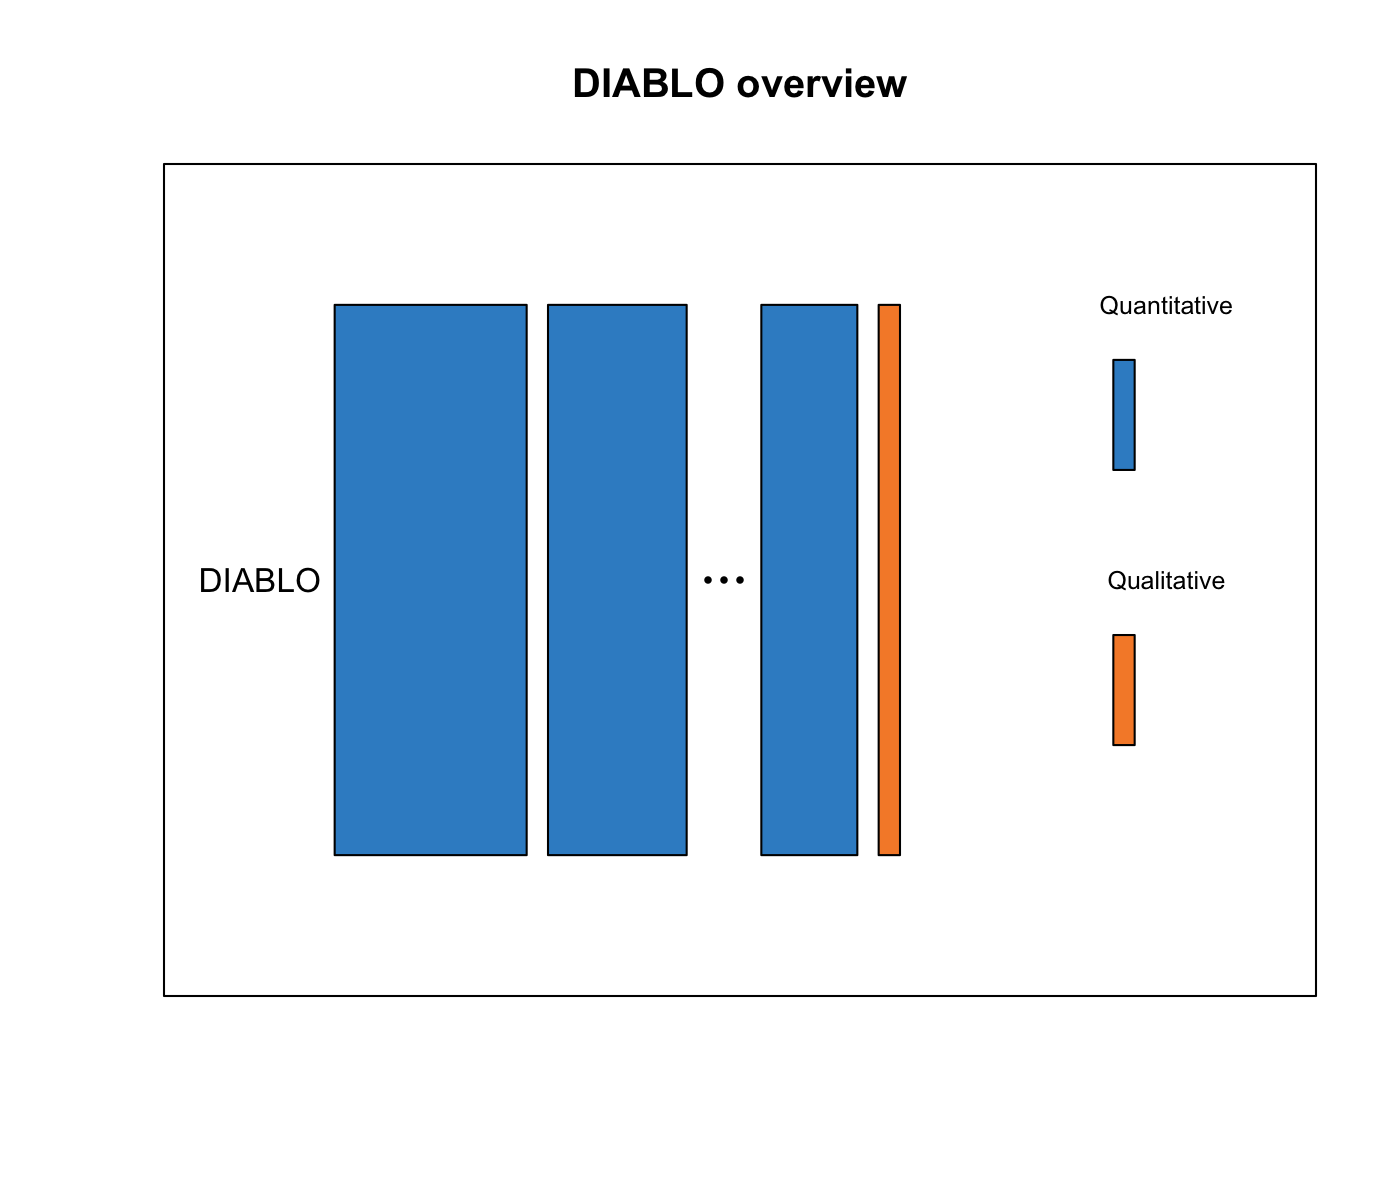
\includegraphics[width=0.5\linewidth]{Figures/overview-DIABLO-1} \end{center}

DIABLO is our new framework in \texttt{mixOmics} that extends PLS for
multiple data sets integration and PLS-discriminant analysis. The
acronyms stands for \textbf{D}ata \textbf{I}ntegration \textbf{A}nalysis
for \textbf{B}iomarker discovery using a \textbf{L}atent
c\textbf{O}mponents \citep{Sin16}.

\section{Biological question}\label{biological-question-4}

{ \emph{I would like to identify a highly correlated multi-omics
signature discriminating known groups of samples.} }

\section{\texorpdfstring{The \texttt{breast.TCGA}
study}{The breast.TCGA study}}\label{the-breast.tcga-study}

Human breast cancer is a heterogeneous disease in terms of molecular
alterations, cellular composition, and clinical outcome. Breast tumours
can be classified into several subtypes, according to levels of mRNA
expression {[}\citet{Sor01}. Here we consider a subset of data generated
by The Cancer Genome Atlas Network \citep{TCGA12}. For the package, data
were normalised and drastically prefiltered for illustrative purposes
but DIABLO can handle larger data sets, see \citep{mixomics} Table 2.
The data were divided into a training set with a subset of 150 samples
from the mRNA, miRNA and proteomics data, and a test set including 70
samples, but only with mRNA and miRNA data (proteomics missing). The aim
of this integrative analysis is to identify a highly correlated
multi-omics signature discriminating the breast cancer subtypes Basal,
Her2 and LumA.

The \texttt{breast.TCGA} is a list containing training and test sets of
omics data \texttt{data.train} and \texttt{data.test} which both
include:

\begin{itemize}
\item
  \texttt{miRNA}: a data frame with 150 (70) rows and 184 columns in the
  training (test) data set for the miRNA expression levels.
\item
  \texttt{mRNA}: a data frame with 150 (70) rows and 520 columns in the
  training (test) data set for the mRNA expression levels.
\item
  \texttt{protein}: a data frame with 150 rows and 142 columns in the
  training data set only for the protein abundance.
\item
  \texttt{subtype}: a factor indicating the breast cancer subtypes in
  the training (length of 150) and test (length of 70) sets.
\end{itemize}

More details can be found in \texttt{?breast.TCGA}.

To illustrate DIABLO, we will integrate the expression levels of miRNA,
mRNA and the abundance of proteins while discriminating the subtypes of
breast cancer, then predict the subtypes of the test samples in the test
set.

\section{Principle of DIABLO}\label{principle-of-diablo}

The core DIABLO method extends Generalised Canonical Correlation
Analysis \citep{Ten11}, which contrary to what its name suggests,
generalises PLS for multiple matching datasets, and the sparse sGCCA
method \citep{Ten14}. Starting from the R package RGCCA from Tenenhaus
et al, we extended these methods for different types of analyses,
including unsupervised N-integration (\texttt{block.pls},
\texttt{block.spls}) and supervised analyses (\texttt{block.plsda},
\texttt{block.splsda}).

The aim of \textbf{N-integration} with our sparse methods is to identify
correlated (or co-expressed) variables measured on heterogeneous data
sets which also explain the categorical outcome of interest (supervised
analysis). The multiple data integration task is not trivial, as the
analysis can be strongly affected by the variation between manufacturers
or 'omics technological platforms despite being measured on the same
biological samples. Before you embark on data integration, we strongly
suggest individual or paired analyses with sPLS-DA and PLS to first
understand the major sources of variation in each data set and to guide
the integration process.

More methodological details can be found in \citep{Sin16}.

\section{Inputs and outputs}\label{inputs-and-outputs-2}

We consider as input a list \texttt{X} of data frames with \(n\) rows
(the number of samples) and different number of variations in each data
frame. \texttt{Y} is a factor vector of length \(n\) that indicates the
class of each sample. Internally and similar to PLS-DA in Chapter
\ref{plsda} it will be coded as a dummy matrix.

DIABLO main outputs are:

\begin{itemize}
\item
  A \textbf{set of components}, also called latent variables associated
  to each data set. There are as many components as the chosen dimension
  of DIABLO.
\item
  A \textbf{set of loading vectors}, which are coefficients assigned to
  each variable to define each component. Those coefficients indicate
  the importance of each variable in DIABLO. Importantly, each loading
  vector is associated to a particular component. Loading vectors are
  obtained so that the covariance between a linear combination of the
  variables from \texttt{X} (the X-component) and from \texttt{Y} (the
  \(Y\)-component) is maximised.
\item
  A \textbf{list of selected variables} from each data set and
  associated to each component if sparse DIABLO is applied.
\end{itemize}

\section{Set up the data}\label{set-up-the-data-2}

We first set up the input data as a list of data frames \texttt{X}
expression matrix and \texttt{Y} as a factor indicating the class
membership of each sample. Each data frame in \texttt{X} should be
\textbf{named} consistently to match with the \texttt{keepX} parameter.

We check that the dimensions are correct and match. We then set up
arbitrarily the number of variables \texttt{keepX} that we wish to
select in each data set and each component.

\begin{Shaded}
\begin{Highlighting}[]
\KeywordTok{library}\NormalTok{(mixOmics)}
\KeywordTok{data}\NormalTok{(breast.TCGA)}
\CommentTok{# extract training data and name each data frame}
\NormalTok{X <-}\StringTok{ }\KeywordTok{list}\NormalTok{(}\DataTypeTok{mRNA =}\NormalTok{ breast.TCGA}\OperatorTok{$}\NormalTok{data.train}\OperatorTok{$}\NormalTok{mrna, }
          \DataTypeTok{miRNA =}\NormalTok{ breast.TCGA}\OperatorTok{$}\NormalTok{data.train}\OperatorTok{$}\NormalTok{mirna, }
          \DataTypeTok{protein =}\NormalTok{ breast.TCGA}\OperatorTok{$}\NormalTok{data.train}\OperatorTok{$}\NormalTok{protein)}
\NormalTok{Y <-}\StringTok{ }\NormalTok{breast.TCGA}\OperatorTok{$}\NormalTok{data.train}\OperatorTok{$}\NormalTok{subtype}
\KeywordTok{summary}\NormalTok{(Y)}
\end{Highlighting}
\end{Shaded}

\begin{verbatim}
## Basal  Her2  LumA 
##    45    30    75
\end{verbatim}

\begin{Shaded}
\begin{Highlighting}[]
\NormalTok{list.keepX <-}\StringTok{ }\KeywordTok{list}\NormalTok{(}\DataTypeTok{mRNA =} \KeywordTok{c}\NormalTok{(}\DecValTok{16}\NormalTok{, }\DecValTok{17}\NormalTok{), }\DataTypeTok{miRNA =} \KeywordTok{c}\NormalTok{(}\DecValTok{18}\NormalTok{,}\DecValTok{5}\NormalTok{), }\DataTypeTok{protein =} \KeywordTok{c}\NormalTok{(}\DecValTok{5}\NormalTok{, }\DecValTok{5}\NormalTok{))}
\end{Highlighting}
\end{Shaded}

\section{Quick start}\label{quick-start-3}

\begin{Shaded}
\begin{Highlighting}[]
\NormalTok{MyResult.diablo <-}\StringTok{ }\KeywordTok{block.splsda}\NormalTok{(X, Y, }\DataTypeTok{keepX=}\NormalTok{list.keepX)}
\KeywordTok{plotIndiv}\NormalTok{(MyResult.diablo)}
\end{Highlighting}
\end{Shaded}

\begin{Shaded}
\begin{Highlighting}[]
\KeywordTok{plotVar}\NormalTok{(MyResult.diablo)}
\end{Highlighting}
\end{Shaded}

Similar to PLS (Chapter \ref{pls}), DIABLO generates a pair of
components, each associated to each data set. This is why we can
visualise here 3 sample plots. As DIABLO is a supervised method, samples
are represented with different colours depending on their known class.

The variable plot suggest some correlation structure between proteins,
mRNA and miRNA. We will further customize these plots in Sections
\ref{diablo:plotIndiv} and \ref{diablo:plotVar}.

If you were to run \texttt{block.splsda} with this minimal code, you
would be using the following default values:

\begin{itemize}
\tightlist
\item
  \texttt{ncomp\ =\ 2}: the first two PLS components are calculated and
  are used for graphical outputs;
\item
  \texttt{scale\ =\ TRUE}: data are scaled (variance = 1, strongly
  advised here for data integration);
\item
  \texttt{mode\ =\ "regression"}: by default a PLS regression mode
  should be used (see Section \ref{PLS:details} for more details) .
\end{itemize}

We focused here on the sparse version as would like to identify a
minimal multi-omics signature, however, the non sparse version could
also be run with \texttt{block.plsda}:

\begin{Shaded}
\begin{Highlighting}[]
\NormalTok{MyResult.diablo2 <-}\StringTok{ }\KeywordTok{block.plsda}\NormalTok{(X, Y)}
\end{Highlighting}
\end{Shaded}

\section{To go further}\label{to-go-further-1}

\subsection{Customize sample plots}\label{diablo:plotIndiv}

Here is an example of an improved plot, see also Section
\ref{splsda:plotIndiv} for additional sources of inspiration.

\begin{Shaded}
\begin{Highlighting}[]
\KeywordTok{plotIndiv}\NormalTok{(MyResult.diablo, }
          \DataTypeTok{ind.names =} \OtherTok{FALSE}\NormalTok{, }
          \DataTypeTok{legend=}\OtherTok{TRUE}\NormalTok{, }\DataTypeTok{cex=}\KeywordTok{c}\NormalTok{(}\DecValTok{1}\NormalTok{,}\DecValTok{2}\NormalTok{,}\DecValTok{3}\NormalTok{),}
          \DataTypeTok{title =} \StringTok{'BRCA with DIABLO'}\NormalTok{)}
\end{Highlighting}
\end{Shaded}

\begin{center}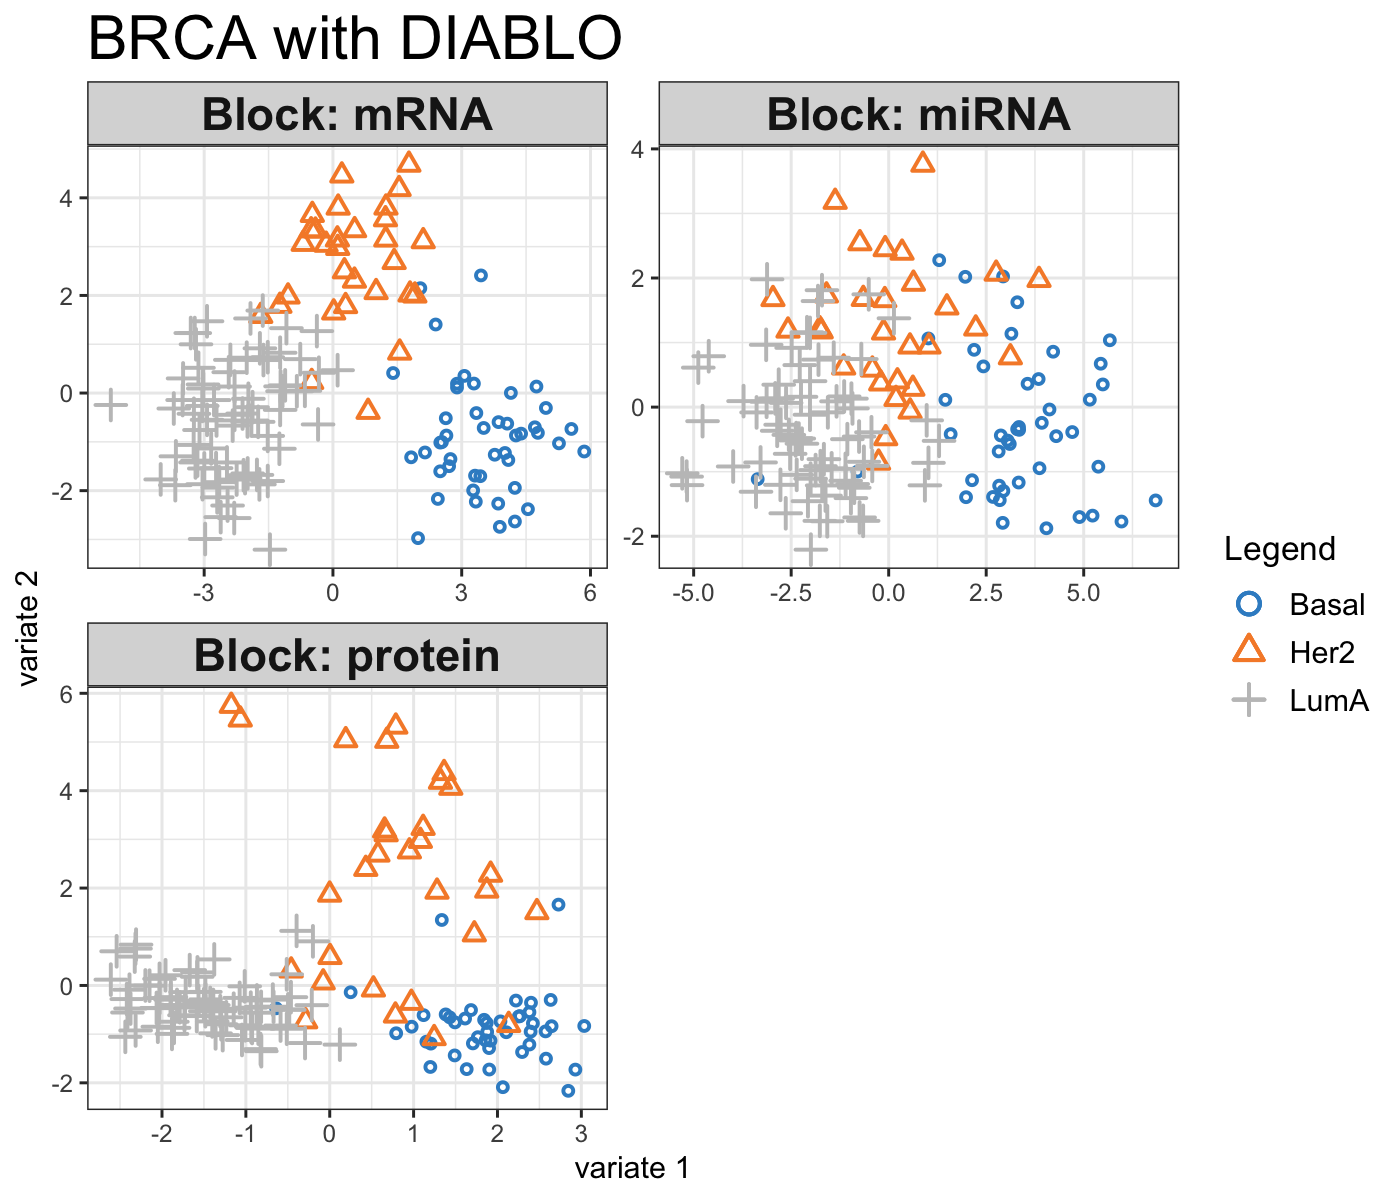
\includegraphics[width=0.5\linewidth]{Figures/unnamed-chunk-4-1} \end{center}

\subsection{Customize variable plots}\label{diablo:plotVar}

Labels can be omitted in some data sets to improve readability. For
example her we only show the name of the proteins:

\begin{Shaded}
\begin{Highlighting}[]
\KeywordTok{plotVar}\NormalTok{(MyResult.diablo, }\DataTypeTok{var.names =} \KeywordTok{c}\NormalTok{(}\OtherTok{FALSE}\NormalTok{, }\OtherTok{FALSE}\NormalTok{, }\OtherTok{TRUE}\NormalTok{),}
        \DataTypeTok{legend=}\OtherTok{TRUE}\NormalTok{, }\DataTypeTok{pch=}\KeywordTok{c}\NormalTok{(}\DecValTok{16}\NormalTok{,}\DecValTok{16}\NormalTok{,}\DecValTok{1}\NormalTok{))}
\end{Highlighting}
\end{Shaded}

\begin{center}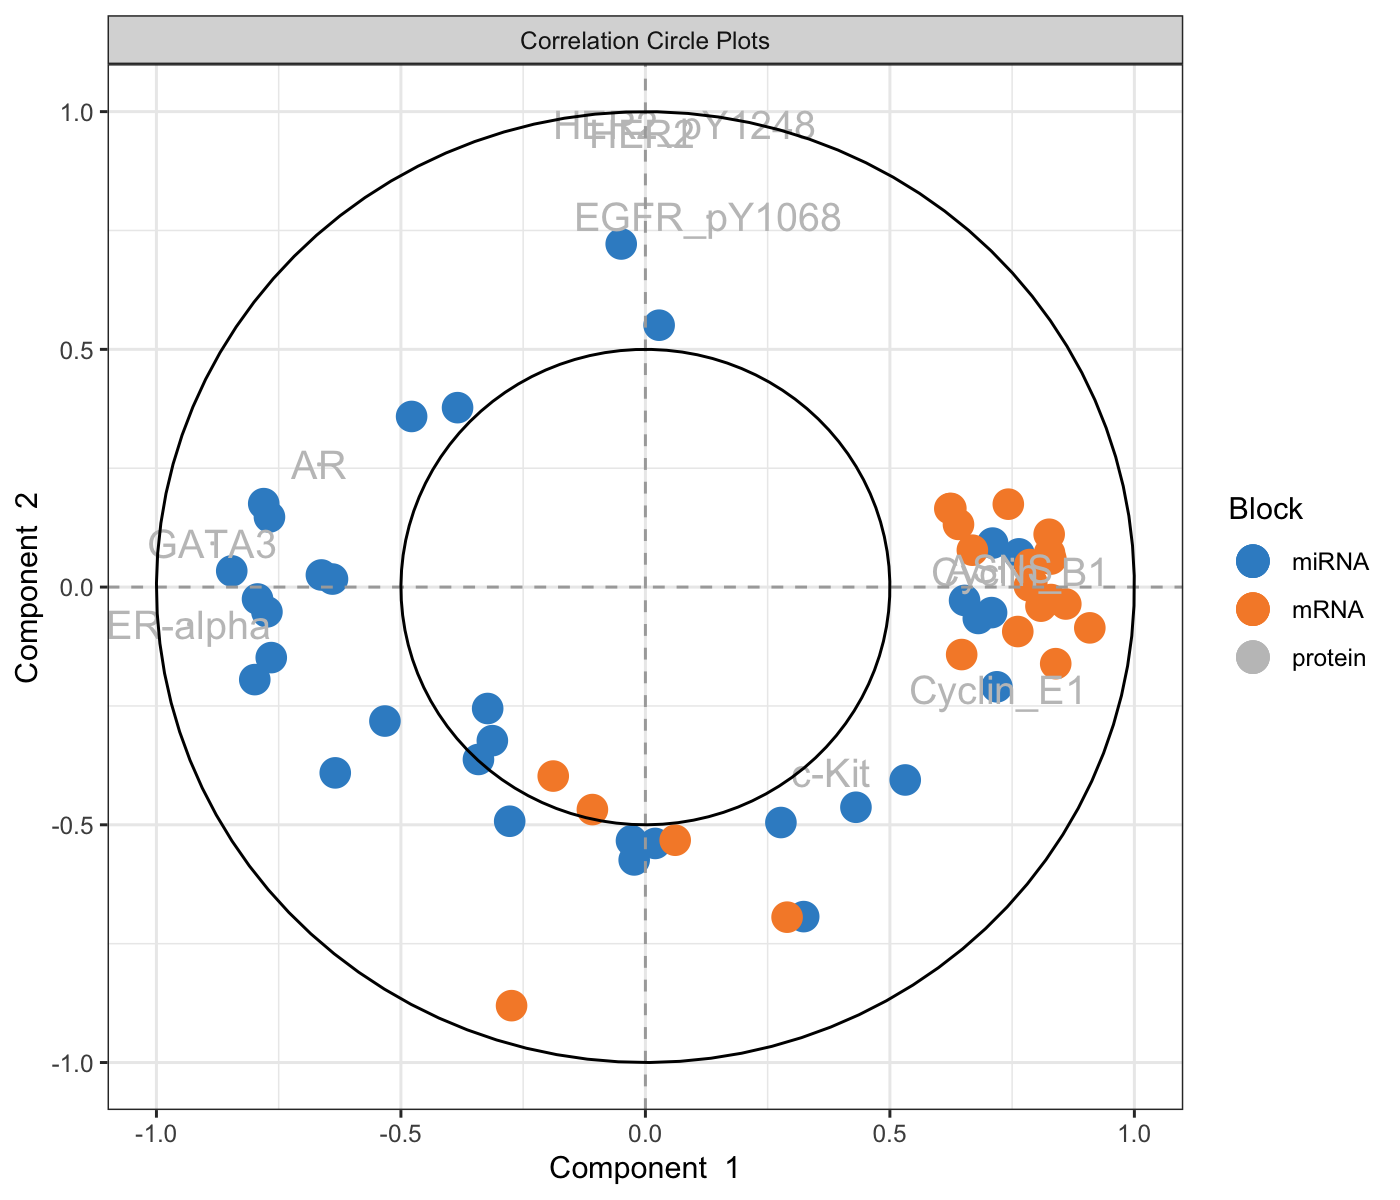
\includegraphics[width=0.5\linewidth]{Figures/unnamed-chunk-5-1} \end{center}

\subsection{Other useful plots for data
integration}\label{other-useful-plots-for-data-integration-1}

Several plots were added for the DIABLO framework.

\subsubsection{\texorpdfstring{\texttt{plotDiablo}}{plotDiablo}}\label{plotdiablo}

A global overview of the correlation structure at the component level
can be represented with the \texttt{plotDiablo} function. It plots the
components across the different data sets for a given dimension. Colours
indicate the class of each sample.

\begin{Shaded}
\begin{Highlighting}[]
\KeywordTok{plotDiablo}\NormalTok{(MyResult.diablo, }\DataTypeTok{ncomp =} \DecValTok{1}\NormalTok{)}
\end{Highlighting}
\end{Shaded}

\begin{center}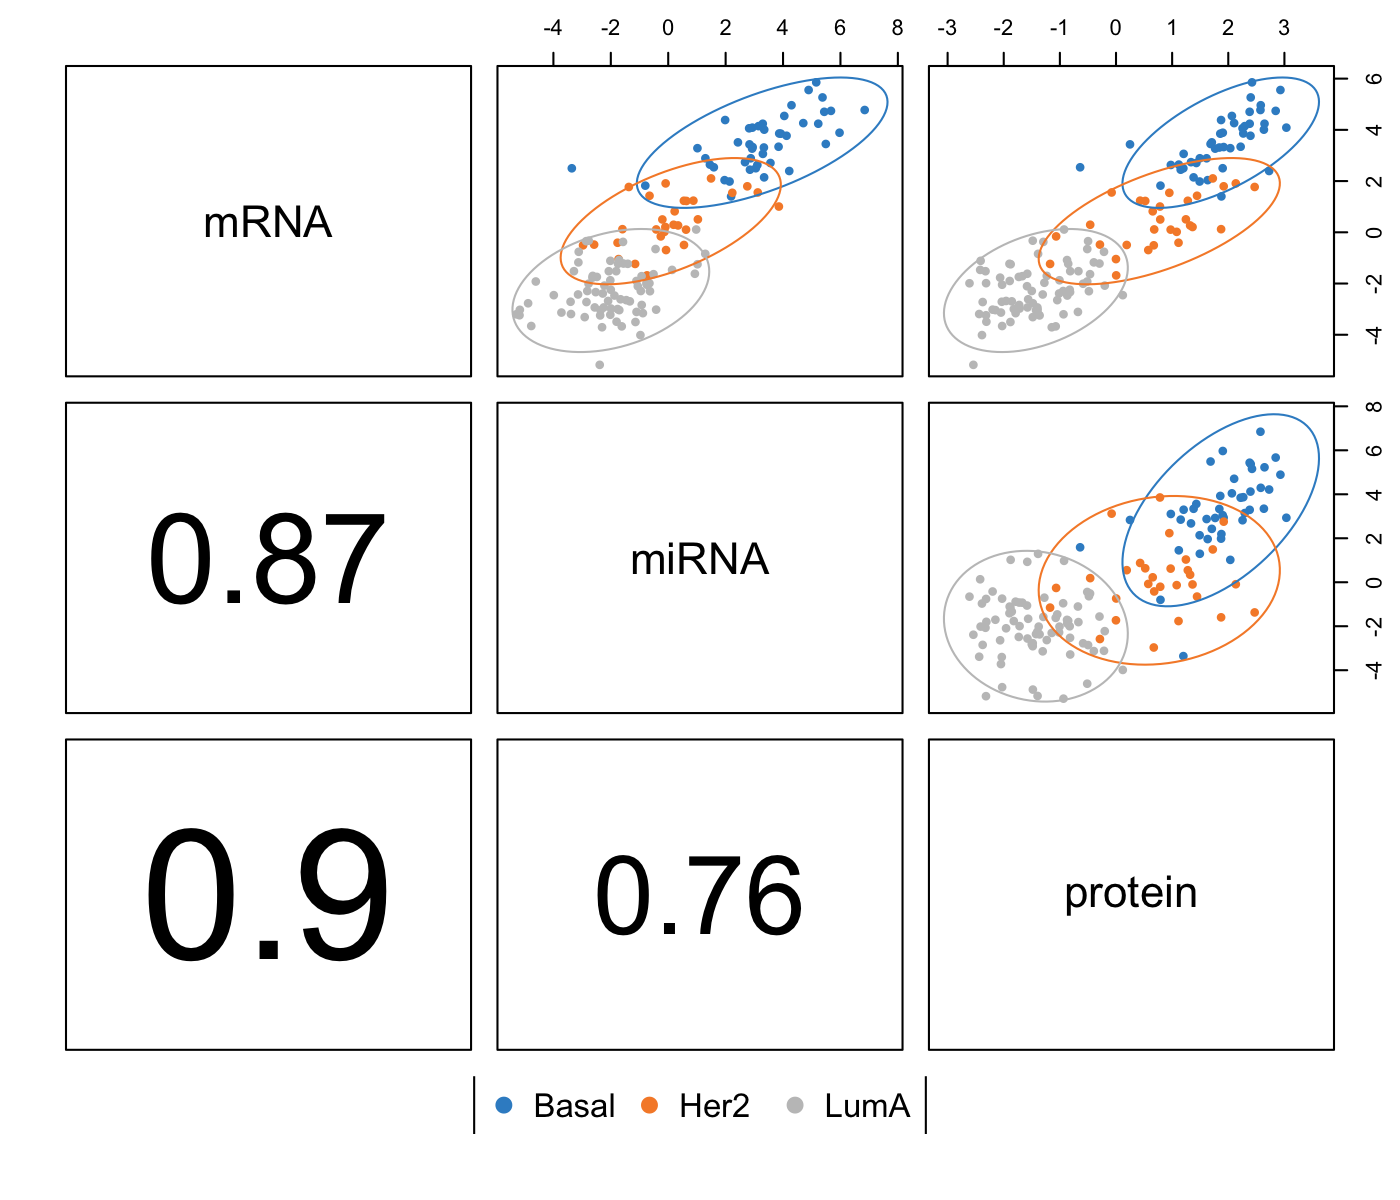
\includegraphics[width=0.5\linewidth]{Figures/unnamed-chunk-6-1} \end{center}

Here, we can see that a strong correlation is extracted by DIABLO
between the mRNA and protein data sets. Other dimensions can be plotted
with the argument \texttt{comp}.

\subsubsection{\texorpdfstring{\texttt{circosPlot}}{circosPlot}}\label{circosplot}

The circos plot represents the correlations between variables of
different types, represented on the side quadrants. Several display
options are possible, to show within and between connexions between
blocks, expression levels of each variable according to each class
(argument \texttt{line\ =\ TRUE}). The circos plot is built based on a
similarity matrix, which was extended to the case of multiple data sets
from \citep{Gon12}. A \texttt{cutoff} argument can be included to
visualise correlation coefficients above this threshold in the
multi-omics signature.

\begin{Shaded}
\begin{Highlighting}[]
\KeywordTok{circosPlot}\NormalTok{(MyResult.diablo, }\DataTypeTok{cutoff=}\FloatTok{0.7}\NormalTok{)}
\end{Highlighting}
\end{Shaded}

\begin{center}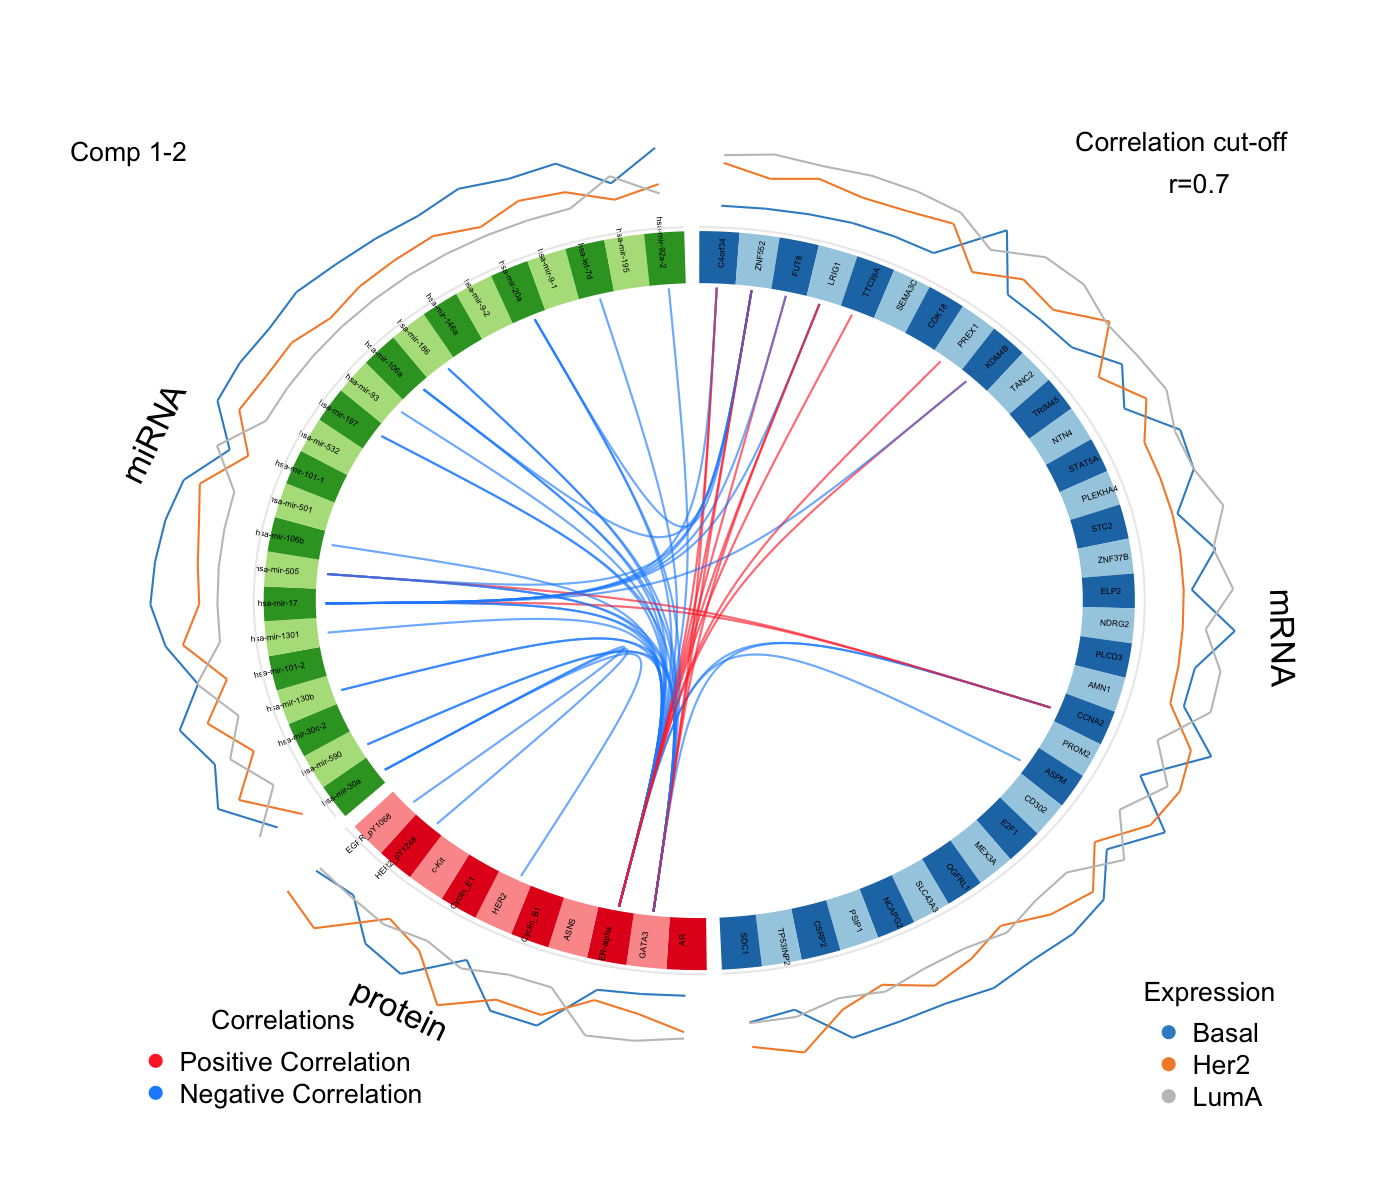
\includegraphics[width=0.5\linewidth]{Figures/unnamed-chunk-7-1} \end{center}

\subsubsection{\texorpdfstring{\texttt{cimDiablo}}{cimDiablo}}\label{cimdiablo}

The \texttt{cimDiablo} function is a clustered image map specifically
implemented to represent the multi-'omics molecular signature expression
for each sample. It is very similar to a classic hierarchical
clustering:

\begin{Shaded}
\begin{Highlighting}[]
\CommentTok{# minimal example with margins improved:}
\CommentTok{# cimDiablo(MyResult.diablo, margin=c(8,20))}

\CommentTok{# extended example:}
\KeywordTok{cimDiablo}\NormalTok{(MyResult.diablo, }\DataTypeTok{color.blocks =} \KeywordTok{c}\NormalTok{(}\StringTok{'darkorchid'}\NormalTok{, }\StringTok{'brown1'}\NormalTok{, }\StringTok{'lightgreen'}\NormalTok{), }\DataTypeTok{comp =} \DecValTok{1}\NormalTok{, }\DataTypeTok{margin=}\KeywordTok{c}\NormalTok{(}\DecValTok{8}\NormalTok{,}\DecValTok{20}\NormalTok{), }\DataTypeTok{legend.position =} \StringTok{"right"}\NormalTok{)}
\end{Highlighting}
\end{Shaded}

\subsubsection{\texorpdfstring{\texttt{plotLoadings}}{plotLoadings}}\label{plotloadings}

The \texttt{plotLoadings} function visualises the loading weights of
each selected variables on each component (default is
\texttt{comp\ =\ 1}) and each data set. The color indicates the class in
which the variable has the maximum level of expression
(\texttt{contrib\ =\ "max"}) or minimum (\texttt{contrib\ ="min"}), on
average (\texttt{method="mean"}) or using the median
(\texttt{method\ ="median"}). We only show the last plot here:

\begin{Shaded}
\begin{Highlighting}[]
\CommentTok{#plotLoadings(MyResult.diablo, contrib = "max")}
\KeywordTok{plotLoadings}\NormalTok{(MyResult.diablo, }\DataTypeTok{comp =} \DecValTok{2}\NormalTok{, }\DataTypeTok{contrib =} \StringTok{"max"}\NormalTok{)}
\end{Highlighting}
\end{Shaded}

\begin{center}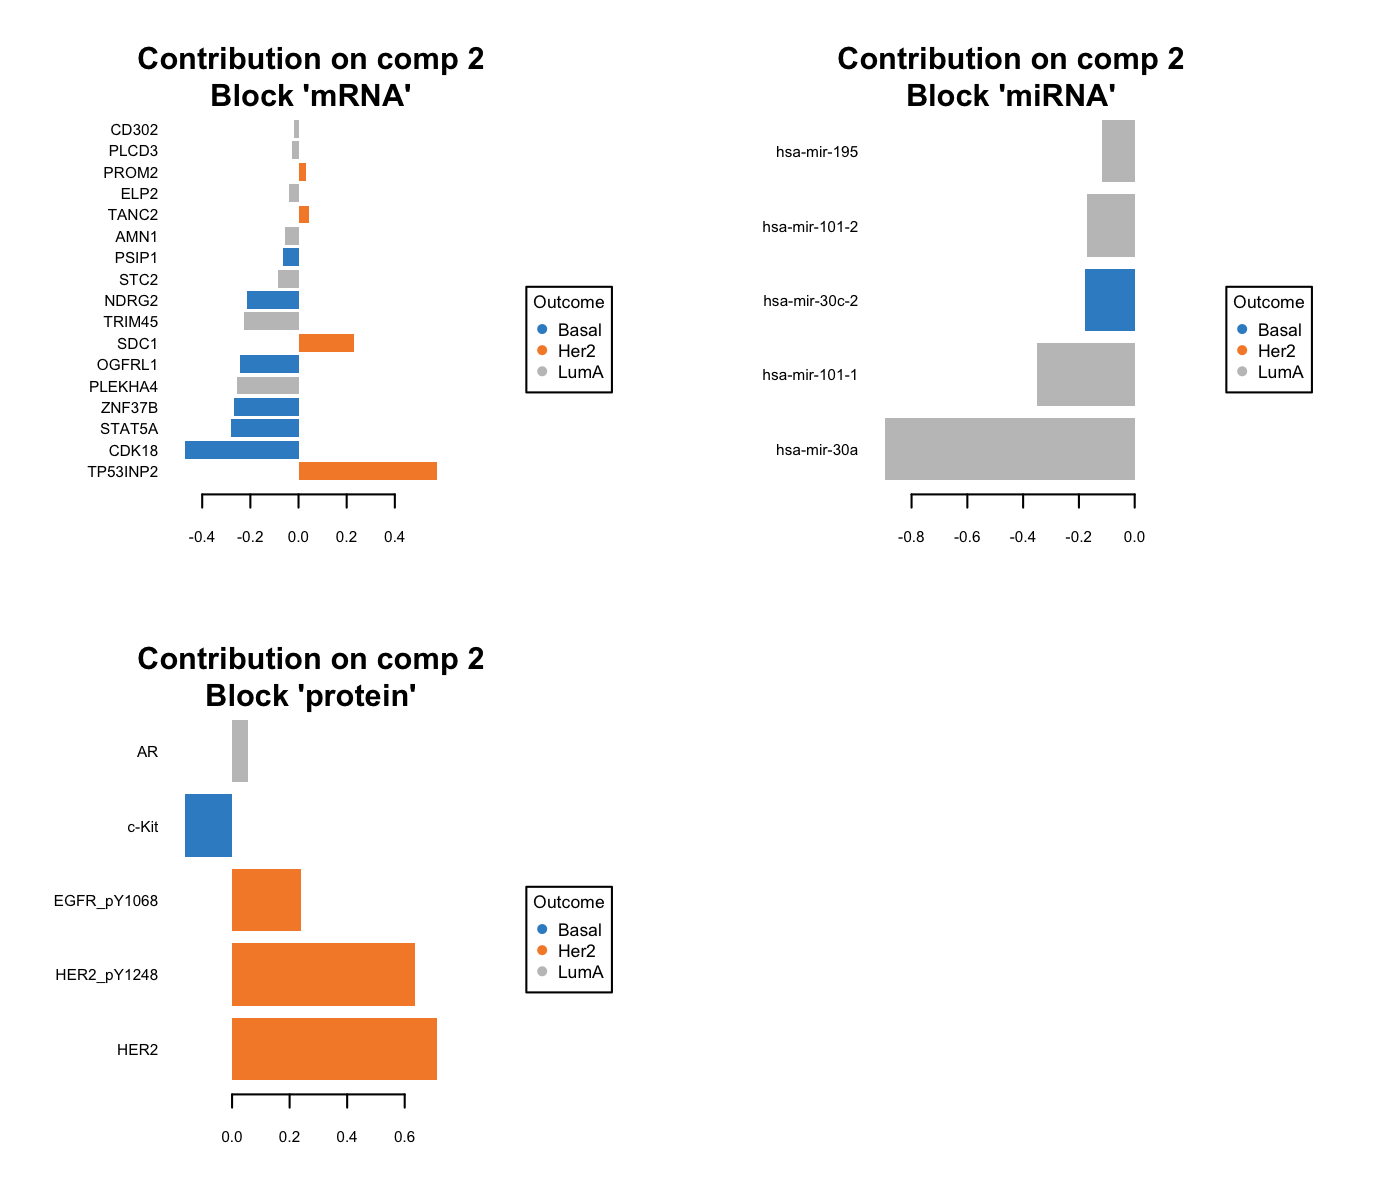
\includegraphics[width=0.5\linewidth]{Figures/unnamed-chunk-9-1} \end{center}

\subsubsection{Relevance networks}\label{relevance-networks}

Another visualisation of the correlation between the different types of
variables is the relevance network, which is also built on the
similarity matrix \citep{Gon12}. Each color represents a type of
variable. A threshold can also be set using the argument
\texttt{cutoff}.

See also Section \ref{pls:network} to save the graph and the different
options, or \texttt{?network}.

\begin{Shaded}
\begin{Highlighting}[]
\KeywordTok{network}\NormalTok{(MyResult.diablo, }\DataTypeTok{blocks =} \KeywordTok{c}\NormalTok{(}\DecValTok{1}\NormalTok{,}\DecValTok{2}\NormalTok{,}\DecValTok{3}\NormalTok{),}
        \DataTypeTok{color.node =} \KeywordTok{c}\NormalTok{(}\StringTok{'darkorchid'}\NormalTok{, }\StringTok{'brown1'}\NormalTok{, }\StringTok{'lightgreen'}\NormalTok{), }
        \DataTypeTok{cutoff =} \FloatTok{0.6}\NormalTok{, }\DataTypeTok{save =} \StringTok{'jpeg'}\NormalTok{, }\DataTypeTok{name.save =} \StringTok{'DIABLOnetwork'}\NormalTok{)}
\end{Highlighting}
\end{Shaded}

\section{Numerical outputs}\label{numerical-outputs}

\subsection{Classification
performance}\label{classification-performance}

Similar to what is described in Section \ref{tuning:sPLSDA} we use
repeated cross-validation with \texttt{perf} to assess the prediction of
the model. For this complex classification problems, often a centroid
distance is suitable, see details in \citep{mixomics} Suppl. Material
S1.

\begin{Shaded}
\begin{Highlighting}[]
\KeywordTok{set.seed}\NormalTok{(}\DecValTok{123}\NormalTok{) }\CommentTok{# for reproducibility in this vignette}
\NormalTok{MyPerf.diablo <-}\StringTok{ }\KeywordTok{perf}\NormalTok{(MyResult.diablo, }\DataTypeTok{validation =} \StringTok{'Mfold'}\NormalTok{, }\DataTypeTok{folds =} \DecValTok{5}\NormalTok{, }
                   \DataTypeTok{nrepeat =} \DecValTok{10}\NormalTok{, }
                   \DataTypeTok{dist =} \StringTok{'centroids.dist'}\NormalTok{)}

\CommentTok{#MyPerf.diablo  # lists the different outputs}

\CommentTok{# Performance with Majority vote}
\CommentTok{#MyPerf.diablo$MajorityVote.error.rate}
\end{Highlighting}
\end{Shaded}

\subsection{AUC}\label{auc}

An AUC plot per block is plotted using the function \texttt{auroc} see
\citep{mixomics}for the interpretation of such output as the ROC and AUC
criteria are not particularly insightful in relation to the performance
evaluation of our methods, but can complement the statistical analysis.

Here we evaluate the AUC for the model that includes 2 components in the
miRNA data set.

\begin{center}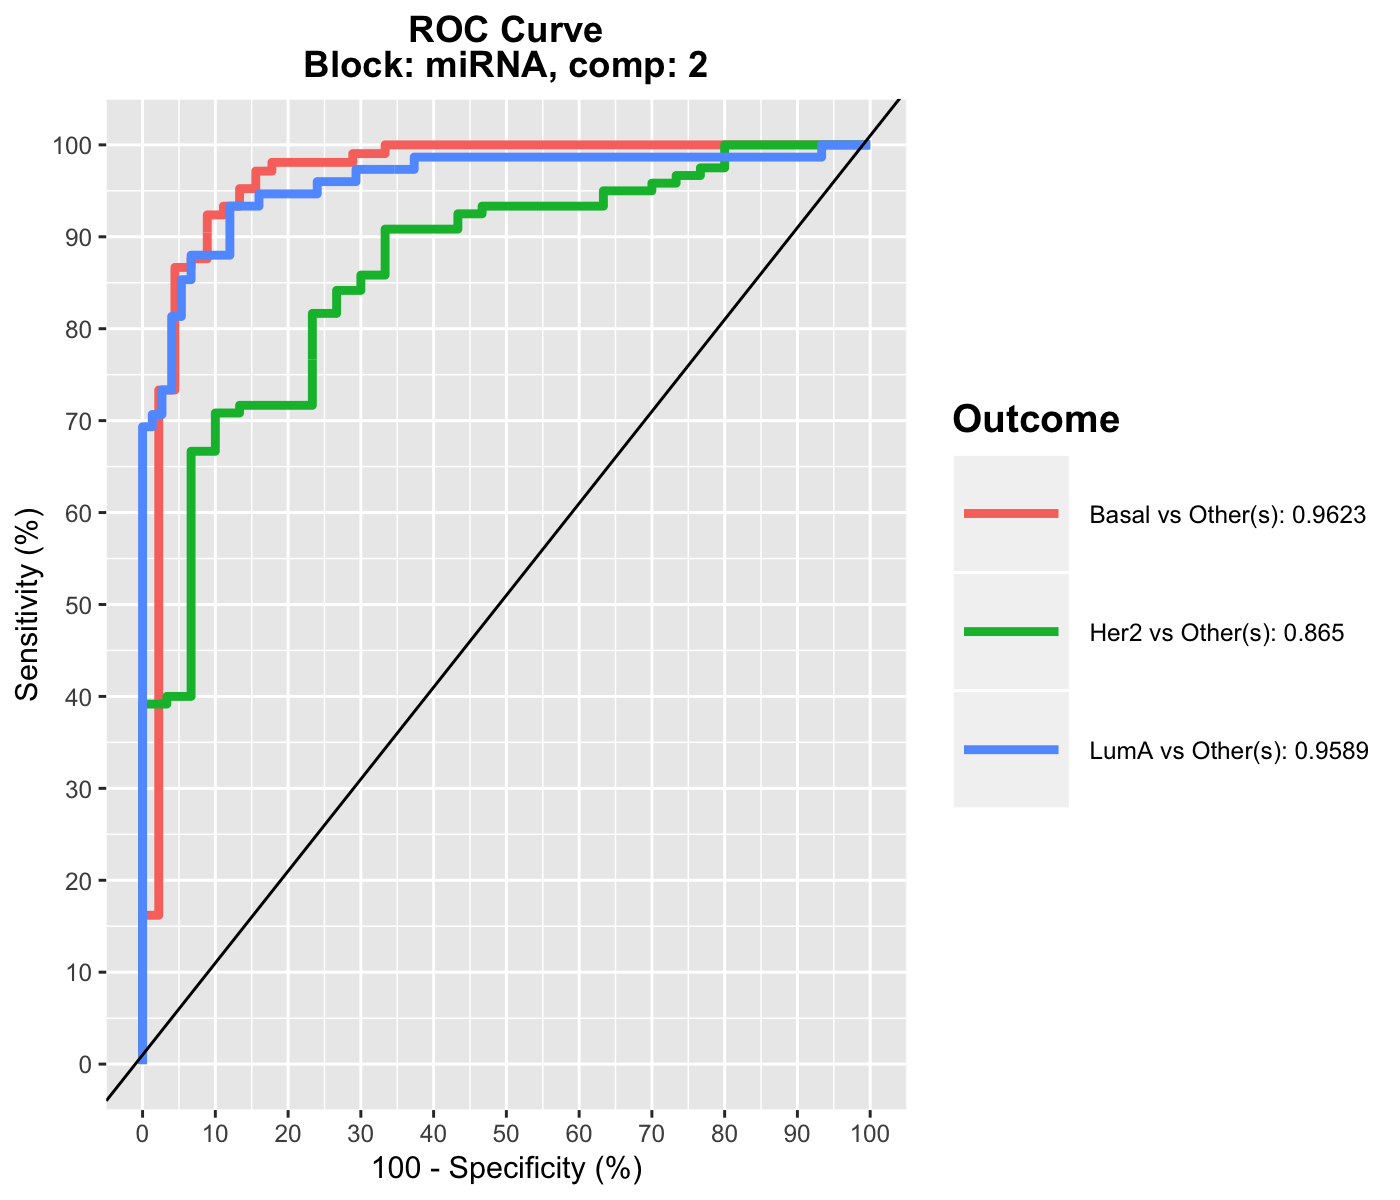
\includegraphics[width=0.5\linewidth]{Figures/unnamed-chunk-12-1} \end{center}

\subsubsection{Prediction on an external test
set}\label{prediction-on-an-external-test-set}

The \texttt{predict} function predicts the class of samples from a test
set. In our specific case, one data set is missing in the test set but
the method can still be applied. Make sure the name of the blocks
correspond exactly.

\begin{Shaded}
\begin{Highlighting}[]
\CommentTok{# prepare test set data: here one block (proteins) is missing}
\NormalTok{X.test <-}\StringTok{ }\KeywordTok{list}\NormalTok{(}\DataTypeTok{mRNA =}\NormalTok{ breast.TCGA}\OperatorTok{$}\NormalTok{data.test}\OperatorTok{$}\NormalTok{mrna, }
                      \DataTypeTok{miRNA =}\NormalTok{ breast.TCGA}\OperatorTok{$}\NormalTok{data.test}\OperatorTok{$}\NormalTok{mirna)}

\NormalTok{Mypredict.diablo <-}\StringTok{ }\KeywordTok{predict}\NormalTok{(MyResult.diablo, }\DataTypeTok{newdata =}\NormalTok{ X.test)}
\CommentTok{# the warning message will inform us that one block is missing}
\CommentTok{#Mypredict.diablo # list the different outputs}
\end{Highlighting}
\end{Shaded}

The confusion table compares the real subtypes with the predicted
subtypes for a 2 component model, for the distance of interest:

\begin{Shaded}
\begin{Highlighting}[]
\NormalTok{confusion.mat <-}\StringTok{ }\KeywordTok{get.confusion_matrix}\NormalTok{(}
                \DataTypeTok{truth =}\NormalTok{ breast.TCGA}\OperatorTok{$}\NormalTok{data.test}\OperatorTok{$}\NormalTok{subtype, }
                \DataTypeTok{predicted =}\NormalTok{ Mypredict.diablo}\OperatorTok{$}\NormalTok{MajorityVote}\OperatorTok{$}\NormalTok{centroids.dist[,}\DecValTok{2}\NormalTok{])}
\KeywordTok{kable}\NormalTok{(confusion.mat)}
\end{Highlighting}
\end{Shaded}

\begin{tabular}{l|r|r|r|r}
\hline
  & predicted.as.Basal & predicted.as.Her2 & predicted.as.LumA & predicted.as.NA\\
\hline
Basal & 15 & 1 & 0 & 5\\
\hline
Her2 & 0 & 11 & 0 & 3\\
\hline
LumA & 0 & 0 & 27 & 8\\
\hline
\end{tabular}

\begin{Shaded}
\begin{Highlighting}[]
\KeywordTok{get.BER}\NormalTok{(confusion.mat)}
\end{Highlighting}
\end{Shaded}

\begin{verbatim}
## [1] 0.2428571
\end{verbatim}

\subsection{Tuning parameters}\label{tuning-parameters-1}

For DIABLO, the parameters to tune are:

1 - The design matrix \texttt{design} indicates which data sets, or
blocks should be connected to maximise the covariance between
components, and to which extend. A compromise needs to be achieved
between maximising the correlation between data sets (design value
between 0.5 and 1) and maximising the discrimination with the outcome
\texttt{Y} (design value between 0 and 0.5), see \citep{Sin16} for more
details.

2 - The number of components to retain \texttt{ncomp}. The rule of thumb
is usually \(K-1\) where \(K\) is the number of classes, but it is worth
testing a few extra components.

3 - The number of variables to select on each component and on each data
set in the list \texttt{keepX}.

For \textbf{item 1}, by default all data sets are linked as follows:

\begin{Shaded}
\begin{Highlighting}[]
\NormalTok{MyResult.diablo}\OperatorTok{$}\NormalTok{design}
\end{Highlighting}
\end{Shaded}

\begin{verbatim}
##         mRNA miRNA protein Y
## mRNA       0     1       1 1
## miRNA      1     0       1 1
## protein    1     1       0 1
## Y          1     1       1 0
\end{verbatim}

The \texttt{design} can be changed as follows. By default each data set
will be linked to the \texttt{Y} outcome.

\begin{Shaded}
\begin{Highlighting}[]
\NormalTok{MyDesign <-}\StringTok{ }\KeywordTok{matrix}\NormalTok{(}\KeywordTok{c}\NormalTok{(}\DecValTok{0}\NormalTok{, }\FloatTok{0.1}\NormalTok{, }\FloatTok{0.3}\NormalTok{,}
                     \FloatTok{0.1}\NormalTok{, }\DecValTok{0}\NormalTok{, }\FloatTok{0.9}\NormalTok{,}
                     \FloatTok{0.3}\NormalTok{, }\FloatTok{0.9}\NormalTok{, }\DecValTok{0}\NormalTok{),}
                   \DataTypeTok{byrow=}\OtherTok{TRUE}\NormalTok{,}
                   \DataTypeTok{ncol =} \KeywordTok{length}\NormalTok{(X), }\DataTypeTok{nrow =} \KeywordTok{length}\NormalTok{(X),}
                 \DataTypeTok{dimnames =} \KeywordTok{list}\NormalTok{(}\KeywordTok{names}\NormalTok{(X), }\KeywordTok{names}\NormalTok{(X)))}
\NormalTok{MyDesign}
\end{Highlighting}
\end{Shaded}

\begin{verbatim}
##         mRNA miRNA protein
## mRNA     0.0   0.1     0.3
## miRNA    0.1   0.0     0.9
## protein  0.3   0.9     0.0
\end{verbatim}

\begin{Shaded}
\begin{Highlighting}[]
\NormalTok{MyResult.diablo.design <-}\StringTok{ }\KeywordTok{block.splsda}\NormalTok{(X, Y, }\DataTypeTok{keepX=}\NormalTok{list.keepX, }\DataTypeTok{design=}\NormalTok{MyDesign)}
\end{Highlighting}
\end{Shaded}

\textbf{Items 2 and 3} can be tuned using repeated cross-validation, as
we described in Chapter \ref{plsda}. A detailed tutorial is provided on
our \href{http://mixomics.org/mixdiablo/}{website} in the different
DIABLO tabs.

\section{Additional resources}\label{additional-resources-3}

Additional examples are provided in \texttt{example(block.splsda)} and
in our DIABLO tab in \url{http://www.mixomics.org}. Also have a look at
\citep{Sin16}

\section{FAQ}\label{faq-3}

\begin{itemize}
\tightlist
\item
  When performing a multi-block analysis, how do I choose my design?

  \begin{itemize}
  \tightlist
  \item
    We recommend first relying on some prior biological knowledge you
    may have on the relationship you expect to see between data sets.
    Conduct a few trials on a non sparse version \texttt{block.plsda},
    look at the classification performance with \texttt{perf} and
    \texttt{plotDiablo} before you can decide on your final design.
  \end{itemize}
\item
  I have a small number of samples (n \textless{} 10), should I still
  tune \texttt{keepX}?

  \begin{itemize}
  \tightlist
  \item
    It is probably not worth it. Try with a few \texttt{keepX} values
    and look at the graphical outputs so see if they make sense. With a
    small \(n\) you can adopt an exploratory approach that does not
    require a performance assessment.
  \end{itemize}
\item
  During \texttt{tune} or \texttt{perf} the code broke down
  (\texttt{system\ computationally\ singular}).

  \begin{itemize}
  \tightlist
  \item
    Check that the \(M\) value for your M-fold is not too high compared
    to \(n\) (you want \(n/M > 6 - 8\) as rule of thumb). Try
    leave-one-out instead with
    \texttt{validation\ =\ \textquotesingle{}loo\textquotesingle{}} and
    make sure \texttt{ncomp} is not too large as you are running on
    empty matrices!
  \end{itemize}
\item
  My tuning step indicated the selection of only 1 miRNA\ldots{}

  \begin{itemize}
  \tightlist
  \item
    Choose a grid of keepX values that starts at a higher value
    (e.g.~5). The algorithm found an optimum with only one variable,
    either because it is highly discriminatory or because the data are
    noisy, but it does not stop you from trying for more.
  \end{itemize}
\item
  My Y is continuous, what can I do?

  \begin{itemize}
  \tightlist
  \item
    You can perform a multi-omics regression with \texttt{block.spls}.
    We have not found a way yet to tune the results so you will need to
    adopt an exploratory approach or back yourself up with down stream
    analyses once you have identified a list of highly correlated
    features.
  \end{itemize}
\end{itemize}

\chapter{Session Information}\label{session-information}

\begin{Shaded}
\begin{Highlighting}[]
\KeywordTok{sessionInfo}\NormalTok{()}
\end{Highlighting}
\end{Shaded}

\begin{verbatim}
## R version 3.5.0 (2018-04-23)
## Platform: x86_64-apple-darwin15.6.0 (64-bit)
## Running under: macOS High Sierra 10.13.3
## 
## Matrix products: default
## BLAS: /Library/Frameworks/R.framework/Versions/3.5/Resources/lib/libRblas.0.dylib
## LAPACK: /Library/Frameworks/R.framework/Versions/3.5/Resources/lib/libRlapack.dylib
## 
## locale:
## [1] en_AU.UTF-8/en_AU.UTF-8/en_AU.UTF-8/C/en_AU.UTF-8/en_AU.UTF-8
## 
## attached base packages:
## [1] stats     graphics  grDevices utils     datasets  methods   base     
## 
## loaded via a namespace (and not attached):
##  [1] compiler_3.5.0  backports_1.1.2 bookdown_0.7    magrittr_1.5   
##  [5] rprojroot_1.3-2 tools_3.5.0     htmltools_0.3.6 yaml_2.1.19    
##  [9] Rcpp_0.12.17    stringi_1.2.2   rmarkdown_1.10  knitr_1.20     
## [13] xfun_0.1        stringr_1.3.1   digest_0.6.15   evaluate_0.10.1
\end{verbatim}

\bibliography{mybib.bib}


\end{document}
